% \documentclass{article}
\documentclass[platex,a4j,11pt,dvipdfmx]{jsarticle}
\usepackage[utf8]{inputenc}
\usepackage[T1]{fontenc}
% \usepackage[OTF]{fontenc}
\usepackage{geometry}
\geometry{a4paper, margin=1in}
\usepackage[explicit]{titlesec}
\usepackage{needspace}
\usepackage{etoolbox}
\usepackage{tocbibind}
\usepackage{tcolorbox}

\definecolor{stepheadingbackground}{RGB}{232,240,245}
\titleformat{\subsection}[block]
  {\normalfont\large\bfseries}
  {}
  {0pt}
  {\colorbox{stepheadingbackground}{%
    \parbox{\dimexpr\linewidth-2\fboxsep\relax}{%
      \raggedright\strut\thesubsection\quad #1\strut}}}
\titlespacing*{\subsection}{0pt}{3.25ex plus 1ex minus .2ex}{1.5ex plus .2ex}
\pretocmd{\subsection}{\Needspace{6\baselineskip}}{}{}

\usepackage{amsmath}
\usepackage{amssymb}

\usepackage{pre}
%\usepackage{hyperref}



\title{Part II : 統計学}
\author{}
\date{}


\begin{document}

\maketitle

\tableofcontents

\newpage


\section{統計学的にデータを調べるということ}

  \subsection{わずかな差をしっかりみる}

    あなたはじゃんけんが強いだろうか.

    実はじゃんけんはランダムではない.
    ある調査\footnote{%
    芳沢光雄（桜美林大学）による, 学生725人・延べ11{,}567回のじゃんけんデータに基づく.
    新聞報道を通じて広く知られている.}
    によれば, グー・チョキ・パーの出現比は
    およそ 35 : 32 : 33. ほぼ互角に見えるが, 完全に一様ではない.
    そしてこの程度の差でも, データ数が十分に大きければ「偶然ではない」と言い切れる.
    つまり, 現実に勝つ確率が高いといえるのだ. 
    じゃんけんに統計的な正解があるとすれば, それはパーだ.

    さらに, あいこが絡む場合はもっと有効な手がある. この研究では, あいこの後に手を変える確率はおよそ 78\% とされているのだ.
    グーであいこになったなら, 相手の次の手はパーかチョキが高確率だ. グーはほぼ出てこない.
    ということはパーに勝つチョキを出せば, 負ける確率をかなり減らすことができる. 
    相手の手が読めるなら, それに合わせて自分の手を選べばよいのだ.
  
  \subsection{確率論と統計学}
    確率論と統計学は, 考える向きが反対である.

    確率論は, 不確かさそのものをあつかうための数学であり, 統計学は, 不確かさを前提に判断を下すための数学である.

    たとえばサイコロを振るとき, 次の目が何になるかは振ってみるまで分からない. 
    しかし「6の目が出る確率は1/6」「100回振ればだいたい何回6が出るか」といったことは, 
    振る前から計算できる. 
    このように不確かさの仕組みを理論的に組み立て, 
    そこから出てくるデータの振る舞いを予測するのが, 確率論で考えていることだ.

    一方で統計学では, 手元にデータはあるが, それを生んだ仕組みを直接調べるのは難しい, という状況を想定する. 
    たとえば100人にアンケートをとった結果から, 
    日本人全体の意見がどうなっているかを推し量ったり, 
    あるいはじゃんけんを11{,}567回観察した結果から, 
    人がじゃんけんで出す手にどんなクセがあるかを読み取ったりする. 
    データは出発点であり, これらは知りたい全体の情報からみると不完全なものだが, 
    それでもこのデータから背後の仕組みに対して何が言えるのか, ということを考えていくのが統計学である.

  \subsection{目標をかたちにする}

    とはいえ, 実際にデータを目の前にしてみると話は別である. 
    内心では「面倒だ」「とりあえず誰かに任せたい」と感じてしまうのが人情である. 
    しかし「これが分かれば儲かる仕事の判断材料になる」「ここに違和感の正体があるかもしれない」といった見通しが立つと, 
    ちょっとやってみるかな, という気になってくる（かもしれない）. 
    その分かれ目は, 「自分は何を知りたいのか」を言葉にできているかどうかにある.

    目的は最初から明確でなくてもいい. 「売上が伸びている気がする, なぜだろう」くらいの
    ぼんやりした問いで十分だ. 数値や図を見ながら問いを絞り込んでいく, その過程そのものが分析である.

    そもそも統計的分析に, 必ずこうしなければならないという手順はない. 
    データと目的次第で, 手法も順序も変わるし, 行きつ戻りつが普通だ. 
    本書では問いをどう立てるかという問題設定の方法論そのものには踏み込まないが, 
    どの章を読んでいるときも 「自分はいま何を明らかにしようとしているのか」を頭の片隅に置いておいてほしい. 
    それだけで, 手法の意味がずっと掴みやすくなるはずだ.

  \subsection{理解してほしいこと}

    本書では, データからどうやって有用な情報をとりだすか, という統計学の実学的な側面を扱う.
    このとき鍵となる概念はそれほど多くない. 
    それは平均と分散, そして正規分布である.
    この三つの概念がどういうものなのか, なぜ重要なのか, 
    それをつかめば統計学の入門としては概ね十分である.

  \subsection{分析の準備}

    本書を通じて, ひとつの共通したデータを手がかりに分析を進めていく.
    扱うのは「コンテンツの人気と評価」に関するデータだ.
    具体的な題材と変数の設計については後で紹介する.

    % ランニング例（題材・表・問い）をここに挿入

    ここで, 統計で使う最も基本的な言葉を確認しておこう.
    手元にあるデータは, 世界のごく一部を切り取ったものにすぎない.
    この切り取られた一部分であるデータを\textbf{標本}と呼び, その背後にある全体を\textbf{母集団}と呼ぶ.
    厄介なことに, 標本はどんな取り方をしても必ずどこかに偏りや情報の欠けを持ってしまう. 
    基本的に完全なデータなど存在しないのだ.
    統計学はそうした不完全な標本を出発点とする. だから,
    「どんなことを, どこまで確からしく語れるのか」についてはいつも意識しておかなければならない.

    各章では, その手法を説明するのに適したデータを使う. 章末ではこの例に戻ってきて, 学んだ手法を当てはめてみる. 全章を通した一貫した分析というには少し届かないかもしれないが, 同じデータを別の手法で見ることで, 各手法の役割がはっきりするはずだ.

\begin{tcolorbox}[
  colback=gray!5,
  colframe=gray!50,
  arc=4mm,
  boxrule=0.5pt,
  title={\textbf{コラム：データとは何か}},
  fonttitle=\large
]

「3, 5, 2, 6」という数字の並びがある.
さて, これは何だろう.
暗証番号かもしれないし, サイコロの出目かもしれない.
実はこれだけでは, 何もわからない.
「あるカフェの月曜から木曜までの売上（万円）」だと聞いて初めて,
この数字は意味のある情報になる.
データとは, 何について, どのように測ったかという文脈があって初めて成り立つものだ.

そして, 文脈があるということは, データにも性格の違いがあるということだ.
売上額や気温のように足し引きに意味がある\textbf{数値データ}もあれば,
天気（晴れ・雨・曇り）や血液型のように分類を表す\textbf{カテゴリデータ}もある.
ちょっと厄介なのは, 数字で書いてあるからといって数値データとは限らないことだ.
たとえばゲームのランキング順位は立派な数字だが,
1位と2位の差と2位と3位の差が同じ意味を持つとは限らない.
あれは量ではなく, 順序を示しているだけである.

性格だけでなく, 姿もさまざまだ.
画像, 音声, テキスト, 人と人のつながり.
データは表の形をしているとは限らない.
しかし本書で扱うのは, 行と列が並んだ, いわゆる表のデータである.
当たり前のようだが, 実はこれ自体がデータの世界のほんの一部にすぎない.
ただ, この「表のデータ」こそが統計の出発点であり,
本書で手を動かしながら付き合っていく相手だ.

\end{tcolorbox}

  % \subsection{本書での前提}

  %   さて, 本書では次のような状況を想定する.

  %   あなたはECサイトで商品を選ぶ際, 他の購入者のレビューや星評価を参考にするだろう.  
  %   「星評価が高い商品はよく売れる」「レビューが多い商品は信頼できる」といった感覚は, 多くの人が持っているかもしれない.  
  %   しかし, 本当にレビューの数や評価の高さは, 商品の売上と統計的に意味のある関係があるのだろうか.

  %   例えば, あなたが運営するECサイトで, 最近販売された商品 20 点について, 次のデータを記録したとする.

  %   \begin{tabular}{ccccc}
  %   \hline
  %   商品ID & 商品カテゴリー & レビュー数 & 星評価平均 & 購買数 \\
  %   \hline
  %   P001 & 家電 & 15 & 4.2 & 120 \\
  %   P002 & 書籍 & 5 & 3.8 & 30 \\
  %   P003 & ファッション & 25 & 4.5 & 200 \\
  %   P004 & 食品 & 10 & 4.0 & 80 \\
  %   P005 & 家電 & 8 & 3.5 & 50 \\
  %   P006 & 書籍 & 2 & 3.0 & 15 \\
  %   P007 & ファッション & 18 & 4.3 & 150 \\
  %   P008 & 食品 & 12 & 4.1 & 90 \\
  %   P009 & 家電 & 30 & 4.8 & 250 \\
  %   P010 & 書籍 & 7 & 3.9 & 40 \\
  %   P011 & ファッション & 22 & 4.4 & 180 \\
  %   P012 & 食品 & 9 & 3.7 & 60 \\
  %   P013 & 家電 & 10 & 3.9 & 70 \\
  %   P014 & 書籍 & 3 & 3.2 & 20 \\
  %   P015 & ファッション & 28 & 4.6 & 220 \\
  %   P016 & 食品 & 14 & 4.2 & 100 \\
  %   P017 & 家電 & 20 & 4.3 & 160 \\
  %   P018 & 書籍 & 6 & 3.6 & 35 \\
  %   P019 & ファッション & 16 & 4.1 & 130 \\
  %   P020 & 食品 & 11 & 4.0 & 75 \\
  %   \hline
  %   \end{tabular}

  %   一見, レビュー数や星評価平均が高い商品ほど購買数が多いように見える.  
  %   だが, その印象が統計的に意味のある関係を示しているのか, それとも偶然の変動で説明できる範囲なのかは, ここからが本題である.  
  %   本書では, この小さな表から実際に手を動かして, 「要約 → 形 → 標本分布 → 推定 → 検定 → 関係 → モデル」という道具立てを順に試し,  
  %   \textbf{売上を伸ばすための具体的な示唆}を, 数と図と文章で導いていく.

% 目的
% ECサイトの購買データを用いて, 商品の売上を伸ばすための具体的な示唆を得る.
%
% （注）統計学は規則性や構造を明らかにし, 必要に応じて因果関係の仮説を検討するための枠組みである.


















% もう少し実用的な例を挙げよう．
% 目の前に大きな湖があるとする．
% もしこの湖にどのくらい魚がいるか見積もってください，と言われたらどのような方法を考えるだろうか．
% 前節の推定をうまく活用すると次のような方法が考えられる．
% まず，魚を一定の数，たとえば100匹ほど捕まえる．
% 次にこの魚にタグをつけて一旦放流し，しばらく待つ．
% そして魚が十分自由に動き回ったと思ったら（一週間程度だろうか）また魚を先ほどと同じ数，100匹捕まえて，タグが付いた魚の数を数える．
% 数えてみた結果，その中にタグの付いた魚が10匹いたとしよう．割合は1/10である．
% するとこの湖には最初にタグをつけた100匹が1/10くらいの割合で存在する, とある程度の確からしさで推測できるので，魚全部ではおよそ1000匹ほどいるだろうと見積もることができる．

% \subsubsection{統計学の起源と進化 - 国家の数字から万人の道具へ}
% 「統計（statistics）」という言葉は, もともと「国家（state）の数字」を意味していたらしい．
% 17世紀のヨーロッパでは人口や税収, 疫病による死亡記録などが集められ始め, 人々はそのデータの中に隠れたパターンや法則があることに気づき始めた. 
% 1662年, ジョン・グラントはロンドンの死亡記録を整理し, 疫病の流行周期や平均寿命を初めて統計的に明らかにした. 
% これが近代統計学のはじまりとされている.

% 18世紀から19世紀にかけて, ラプラス, ガウス, ポアソンといった数学者たちによって確率論が発展し, 統計学の理論的基盤が形成された．
% 20世紀には, R.A.フィッシャーやカール・ピアソンらによって実験計画法や仮説検定の手法が確立され, 統計学は科学研究の必須ツールとなった．

% さらに看護師フローレンス・ナイチンゲールはクリミア戦争の現場で衛生状態を統計データにまとめ, 「ナイチンゲールのバラ」と呼ばれる図を用いて衛生改善の必要性を説いた. 
% 実はこの時代の戦争において, 戦闘行為による直接的な死者よりも, 衛生状況が悪いことによる負傷兵の死者の方が多かったのである. 
% これにより統計は単なる数字遊びではなく, 人々を説得し社会を動かす力を持つことが明らかになった. 

% 現代では, 統計学はビッグデータ, 機械学習, 人工知能といった先端分野を支える基盤となっている．
% かつては専門家だけのものだった高度な統計手法も, コンピュータの発達により広く一般に利用可能になり, 
% ビジネス, 医療, 教育, スポーツ, 芸術など, あらゆる領域で活用されている．

% \subsubsection{標本と統計}
% 改めて統計の言葉遣いについて改めて言及しておこう．
% データとは, 観察や測定によって得られた情報のことを指す. 
% データには様々な特性や属性があり, これらを「変数」と呼ぶ. 
% 変数には, 身長や体重のような数値で表される量的変数と, 性別や血液型のようなカテゴリーで表される質的変数があるが，これらについてはあとで詳しく述べる.
% そして，今，手元にある「データの集まり」のことを標本という．
% 標本は，実際は巨大な全体集合からその一部を取り出したものである．
% この全体集合のことを「母集団」と言い，母集団から標本を取り出すことを「抽出する」という．
% 標本の大きさ, つまりデータの数のことを「標本サイズ」または「サンプルサイズ」と呼ぶ. 例えば, 100人分のデータがあれば, サンプルサイズは100となる.
% 統計的な量（たとえば平均など）を計算したり, データの特徴を図や表で表したりして「今手元にあるデータの理解を深める」ことを「記述統計」と呼ぶ. 
% 一方, 標本から母集団の特徴を推測したり，データの比較をしたりすることを「推測統計」という.
% 統計の項目ではこれら記述統計と推測統計の基本的なこと，つまり何がしたくて，どうやって計算して，なにがわかるのかを理解することを目指す．



% \subsection{データを「見る」ための基礎 - 無秩序から秩序への変換}

% \textbf{数字の羅列に意味を付与する - コンテキストの魔法}\newline
% データは単に文字や数字が並んでいるものではない.
% その並びには必ずなんらかの背景や文脈が存在する.  
% 例えば, 「20, 50, 30, 90, 40, 80, 90」だけでは何を表しているのか意味不明である. 
% しかし, 「1週間の来店人数（月～日）：20, 50, 30, 90, 40, 80, 90人」と文脈が与えられると, 突然意味が生まれる. 
% 水曜日（30人）よりも火曜日（50人）の方が来店者が多く, 週末（土日：80, 90人）に集中していることが分かる.
% これにより, たとえば「週末は人が多いよね」となんとなく思っていたことが事実として現れてくるのである  

% このように, 数字に「タイトル（何についてのデータか）」「ラベル（各値が何を表すか）」「単位（何を数えているのか）」「時間的・空間的文脈（いつ, どこのデータか）」を付与することで, 無秩序な数字の羅列は, 私たちが「見て」解釈できる情報へと変換されるのです. 

% \textbf{「見えない」から「見える」へ：データの文脈化の技術}\newline
% 記録されたままの状態のデータを「生」と表現することがあるが, そのようなデータは非常に扱いにくい状態であることが多い. 
% それを磨き上げ, 形を整えることで初めて宝石としての価値が現れます. データを「見える」ようにするためには, 以下のような文脈化の技術が重要です：

% 1) \textbf{比較対象の設定}：東京の平均気温25℃という数字は, それだけでは「暑い」のか「寒い」のか判断できませんが, 過去10年の同時期の平均が22℃だと分かれば「例年より暑い」と理解できます. 同様に, ある美術展の来場者数5,000人も, 類似の展覧会の平均来場者数と比較することで, その「多さ」や「少なさ」が初めて意味を持ちます. 

% 2) \textbf{時間軸の導入}：データに時間的文脈を加えることで, 変化やトレンドが見えてきます. 例えば, 美術館の月間来場者数を単月で見るより, 過去5年間の推移として見ることで, 季節変動や長期的な人気の変化が明らかになります. 

% 3) \textbf{空間的・地理的文脈}：同じ「美術館の来場者数」でも, 都心に位置する国立美術館と地方の小規模美術館では, 比較の意味が異なります. 地理的条件や施設の規模などの空間的文脈を考慮することが, 公平な比較には不可欠です. 

% 4) \textbf{条件を追加する}：単一の変数だけでなく, 関連する複数の変数と組み合わせることで, より豊かな文脈が生まれます. 例えば, 美術館の来場者数と天気, 交通アクセス, 特別展の有無などを併せて分析することで, 来場者数の変動要因が見えてきます. 


% \textbf{データの尺度と比較可能性 - 同じ土俵で考える}\newline
% データを扱うとき, 必ず意識しなければならないのはそのデータの「単位」である. 
% 同じ「3」という数字でも「3人」と「3cm」と「3秒」では全く異なる情報となり, 比較したりすることがようやく可能となるのである. 
% また, さらに「3点」という評価も, 5点満点なのか10点満点なのかによって意味が変わってくる. 

% 統計学では, データの尺度を以下のように分類します：

% 1) \textbf{名義尺度（nominal scale）}：カテゴリーや分類を表す尺度（例：展示作品のジャンル, 来場者の性別）. 順序や大小関係はなく, 単なる区別のみ. 

% 2) \textbf{順序尺度（ordinal scale）}：順序や優劣を表す尺度（例：展示の満足度評価「とても良い, 良い, 普通, 悪い, とても悪い」）. 大小関係はあるが, 間隔の等間隔性は保証されない. 

% 3) \textbf{間隔尺度（interval scale）}：等間隔性を持つ尺度（例：温度（摂氏）, 日付）. 「ゼロ」という数字の意味がある程度自由に設定され, 絶対的な「無」を表さない. たとえば「摂氏 0 度」は温度が全くないということではないし, 4 月 0 日という日は存在しない.  

% 4) \textbf{比率尺度（ratio scale）}：絶対的なゼロ点を持つ尺度（例：身長, 重さ, 人数）. 比率の比較が意味を持つ（「AはBの2倍」など）. 

% 1, 2 のようなデータはデータどうしで「四則演算」ができないことに注意が必要である. 
% たとえば血液型「A型」と「B型」を足すことは一般的に見て意味不明だと思う. 
% このような場合はたとえば血液型をラベルのように用いて「A型」の「人数」などを数えることにより, 足すことに意味が生まれる. 

% 1,2 のようなデータはカテゴリデータ（あるいは質的データ）と呼ばれ, 3, 4のようなデータは数値データ（あるいは量的データ）と呼ばれる. 
% 本書では量的データの扱いを通して統計学の基礎を身に着けていこう. 
% 質的データに対する基本的な分析についても 3 節で触れる. 


% \subsection{データと表・視覚的整理 - 情報の構造化と可視化}

% \textbf{表が果たす強力な役割 - 情報の地図作り}\newline
% データというと以下のような表を思い浮かべる方も多いのではないだろうか. 
% 大げさに聞こえるかもしれないが, 表は情報を整理するための非常に優れたツールである. 
% 列の名前を見るだけでだいたいどんなことを表すデータなのか把握でき, ピンポイントでほしい情報をすぐに見つけることができる. 

% \begin{tabular}{|l|c|c|c|c|c|}
% \hline
% & 午前 & 昼食時 & 午後 & 夕方 & 合計 \\
% \hline
% 月曜日 & 15 & 20 & 25 & 10 & 70 \\
% 火曜日 & 35 & 45 & 50 & 30 & 160 \\
% 水曜日 & 30 & 40 & 45 & 25 & 140 \\
% 木曜日 & 25 & 35 & 40 & 20 & 120 \\
% 金曜日 & 40 & 50 & 55 & 35 & 180 \\
% 土曜日 & 80 & 100 & 120 & 60 & 360 \\
% 日曜日 & 90 & 110 & 130 & 70 & 400 \\
% \hline
% 合計 & 315 & 400 & 465 & 250 & 1430 \\
% \hline
% \end{tabular}

% この表からは, 「週末（土日）の来場者数が平日の約3倍である」「全体的に午後の時間帯が最も混雑する」「月曜日は最も来場者が少なく, その差は日曜日の約1/6である」といった情報が一目で読み取れます. このような表の「読み方」を身につけることは, データを「見る」ための基本的なスキルです. 

% \textbf{整理の技術：データの見せ方が結論を変える}\newline  
% 表の作り方（ランキング順, 時系列順, カテゴリー別など）の工夫により, データの読み取り方や印象は大きく変わります. 例えば, 同じ美術館の来場者データでも, 「曜日別の集計」と「天気別の集計」では, まったく異なる傾向が浮かび上がります. 

% さらに, どの軸で並べるか, どの値を強調するかによっても印象は変化します. 例えば上記の表を「来場者数の多い順」に並べ替えると：

% \begin{tabular}{|l|c|c|c|c|c|}
% \hline
% & 午前 & 昼食時 & 午後 & 夕方 & 合計 \\
% \hline
% 日曜日 & 90 & 110 & 130 & 70 & 400 \\
% 土曜日 & 80 & 100 & 120 & 60 & 360 \\
% 金曜日 & 40 & 50 & 55 & 35 & 180 \\
% 火曜日 & 35 & 45 & 50 & 30 & 160 \\
% 水曜日 & 30 & 40 & 45 & 25 & 140 \\
% 木曜日 & 25 & 35 & 40 & 20 & 120 \\
% 月曜日 & 15 & 20 & 25 & 10 & 70 \\
% \hline
% 合計 & 315 & 400 & 465 & 250 & 1430 \\
% \hline
% \end{tabular}

% このように並べ替えると, 「曜日による来場者数の差が非常に大きい」ことがより明確になります. 
% データの整理方法自体が, 分析の視点と結論を左右する重要な要素なのです. 

% 統計学では, このような「データの見せ方」そのものが分析の一部であることを認識し, 目的に応じた適切な整理方法を選択することが重要です. 
% 異なる整理方法で同じデータを複数回見ることで, 多角的な理解が可能になります. 

% ほかにも実はスマートフォンに保存されている写真などの画像データは「表」そのものである. 
% 各セルの大きさは「ピクセル」と呼ばれ, それぞれのセルにはそのセルの「色情報」が保存されている. 
% これを特殊な読み取り方をすることによって画像として表示されるのである. 

% \textbf{表からグラフへ：視覚化の第一歩}\newline
% 整理された表は, 数字に意味を与え, 後のグラフや図表による可視化の基盤となります. 
% 人間の脳は, 数字の羅列よりも視覚的なパターンを認識するのが得意です. 
% 例えば, 「月別売上データ」は表よりも折れ線グラフで示した方が, 季節変動や成長トレンドが一目で理解できます. 

% グラフは表の情報を視覚言語に翻訳するものであり, その選択は伝えたいメッセージによって異なります：

% 1) \textbf{時系列データの変化}：折れ線グラフが最適（例：年間を通じた来場者数の変動）

% 2) \textbf{部分と全体の関係}：円グラフや積み上げ棒グラフが有効（例：来場者の年齢層構成）

% 3) \textbf{分布の形状}：ヒストグラムや箱ひげ図が適切（例：滞在時間の分布）

% 4) \textbf{相関関係}：散布図が直観的（例：入場料と来場者数の関係）

% この「表からグラフへ」の変換プロセスは, データを「見る」技術の核心部分です. 
% 適切なグラフ形式を選択し, タイトル, ラベル, 凡例, スケールなどを工夫することで, データの持つメッセージをより効果的に伝えることができます. 

% \textbf{デジタル時代の表現技術 - データ体験の革新}\newline
% 現代のデータ可視化技術は, 静的な表やグラフを超え, インタラクティブなダッシュボード, リアルタイム更新, 3D表現, 拡張・仮想現実（AR/VR）を用いた没入型データ体験など, 多様な方法でデータを「体験」できるツールへと進化しています. 

% 例えば, 美術館の来場データを分析する場合, 従来の静的なグラフだけでなく, 以下のような革新的な可視化が可能になっています：

% 1) \textbf{インタラクティブマップ}：館内の平面図上に来場者の動線や滞在時間をヒートマップで表示し, 人気の展示や混雑エリアを直感的に把握

% 2) \textbf{時間変化アニメーション}：一日の時間帯による来場者の流れを動画のように表現し, 混雑の波を視覚的に理解

% 3) \textbf{多次元データの可視化}：来場者の年齢, 性別, 滞在時間, 支出金額などの多変量データを, 色, 形, 大きさなどの視覚要素に変換して複合的に表現

% これらの先進的なデータ表現技術を効果的に活用するためには, 統計学の基本原則を理解することが不可欠です. 技術は進化しても, 「データを意味ある形で整理し, パターンを見出し, 解釈する」という統計学の本質は変わりません. 現代の視覚化ツールは, この本質的なプロセスをより効率的かつ魅力的に実行するための道具なのです. 

% 統計学の基礎を身につけることは, 現代のデータ豊富な環境で「見る力」を養うための重要なステップです. 
% 数字の羅列から意味のあるストーリーを引き出す能力は, ビジネス, 研究, 芸術, そして日常生活のあらゆる場面で, より良い判断と創造的な問題解決につながるでしょう. 






\newpage

\section{データを要約する}

  \subsection{問い}

    食事に行く店を決める, Amazon で電化製品を選ぶ, そういう場面を思い出してみてほしい.
    こういうとき, とりあえずレビュー評価を確認したりしないだろうか.
    星の平均が4.2の製品と3.1の製品があれば, まず4.2のほうを見てみるといった具合である.

    ここで私たちが無意識に行っていることは「データの要約」と「比較」だ.
    星4.2というのは, 何十人もの評価を1つの数字にまとめた結果である.
    何十人分ものバラバラな評価をそのまま頭で処理するのは無理だから, 代わりに「4.2」という1つの数字を指標にしている.
    そして, 同様にまとめられた「3.1」という数をみて, これは4.2のほうが良さそうだぞ, と判断しているのだ.
    日常的に行っている「たくさんのデータを1つにまとめる」「まとめた数どうしを比べる」という行動は, もっとも身近なデータ分析の一つだ.

    ただ, このやり方だけでいつもよい判断ができるとは限らない.
    同じ星4.0の製品が二つ並んでいたら, 次は何を見て選ぶことになるだろう.
    一つが星5だったとしても, たった一人からの評価しかなかったら, その星5をそのまま信じるのはためらわれる.
    データをまとめてしまうと, その数字以外の情報はどこかへ行ってしまうのだ.

    データの要約とは一体どんなもので, どんな情報がなくなってしまうのだろうか.


  \subsection{平均だけでは見えないもの}

    データを1つの数にまとめる方法でもっともポピュラーなのは, 平均だろう.
    データの値を全部足し合わせて個数で割るだけで求まり, 計算しやすいのが取り柄である.

    しかし, 平均だけを見ていてもうまく拾えないことがある.
    たとえば, 通勤に使う電車の平均遅延時間が「1日あたり2分」だったとする.
    別の路線も平均2分だったとしたら, どちらに乗っても同じような通勤になるだろうか.
    実は片方は毎朝きっちり2分遅れるだけで, もう片方は99\%の日は定刻通りだが残り1\%で200分止まる, ということがありうる.
    同じ平均2分でも, 中身はまるで違うのだ.
    平均という1つの数からは, データが平均のまわりに集まっているのか, それとも遠くまで散らばっているのかが見えない.
    平均だけを頼りに「どちらの路線も同じようなものだろう」と判断してしまうと, 年に数回, 始業に3時間遅れる路線を引き当てることになる.
    平均には現れない\textbf{散らばり}という情報が, ここでは判断を左右している.

    あるいは平均年収のような例もある.
    日本の平均年収は約460万円といわれている\footnote{%
    国税庁「令和5年分民間給与実態統計調査」による. 1年を通じて勤務した給与所得者の平均給与が460万円. 中央値は同調査では公表されていないが, 給与階級別の分布から400万円前後と読み取れる.}が, 実は「平均以下」の年収の人のほうが多数派だ.
    一部の高収入者が全体の平均を引き上げているからである.
    こういうときに使われるのが, データを順番に並べて真ん中に来る値をとる\textbf{中央値}という別のまとめ方だ.
    中央値はだいたい400万円前後で, 平均よりも低い.
    真ん中の順位の人は, 高収入者がどれだけ稼ごうがそう簡単には動かないからである.
    平均460万円という数だけを見て「自分の年収はそれより下だから真ん中以下なんだな」などと捉えると, 実態とはずれた印象を持つことになる.

    平均だけでは, 真ん中の人がどのあたりにいるのかが見えてこない.

    ということは, データのまとめ方は平均だけではないし, それぞれの方法が別の情報を拾っているらしい.
    そもそも「データを1つの数にまとめる」とはどういう操作なのか, 一度整理してみよう.


  \subsection{理論の最小核}

    星4.2の例でやっていたのは, 何十人もの評価を「4.2」という1つの数に置き換えることだった.
    多数の値を1つの数で代表させる, それが要約という操作の中身である.

    なぜわざわざ要約するのかといえば, 大きく2つの利点があるからだ.
    ひとつは, 別の集まりと比べやすくなること.
    冒頭で平均4.2と平均3.1を比べたが, あれもまさに同じことをやっていた.
    別の集まりにそれぞれ同じやり方で要約をかけて, 出てきた数同士を見比べていた.
    バラバラの評価をそのまま眺めて比較するのは難しいが, 1つの数に揃えれば見比べるのはたやすい.

    もうひとつは, その数を「対象そのものの値」として扱えるようになることだ.
    平均4.2の製品があったとき, 私たちはそれを「4.2の価値がある製品」のように受け取る.
    何十人もの評価をまとめた結果にすぎない数字が, いつのまにかその製品自体の値として扱われている.
    こうした置き換えは, 後の章で「推定」という言葉でもう少し丁寧に扱う.
    このように, 要約という操作のおかげで比較や推定が成り立っている.
    一方で前の節で見たように, 要約には情報の欠落がついて回る.
    平均は散らばりを拾わないし, 中央値は全体の合計を語らない.
    どんな要約のしかたも, 必ず何かの情報を犠牲にしている.

    データの要約のしかたはいろいろあるが, 「観測値からひとつの数を計算する」という形そのものは共通している.
    ここで, その数に名前を付けておこう.

    \begin{defi}{統計量}{stat}
      $n$個の観測値 $x_1, x_2, \ldots, x_n$ から計算される数を\textbf{統計量}と呼ぶ.
    \end{defi}

    「観測値から計算される数」というのは, 観測値が決まればおのずと値が定まる, ということだ.
    平均にせよ中央値にせよ, 同じ観測値を与えれば計算結果は同じ数になるので, いずれも統計量だ.
    だから統計量というのは特定の「数」というより, 「観測値を入れると数が出てくるなんらかの手続き」というイメージに近い.

    「平均」「中央値」というのも, 個別の値そのものではなく, それぞれの手続きの名前なのだ.
    どんな統計量を使うかは, 何を読み取って何を捨てるかの選び方でもある.

    年収の例では, 高収入者に引きずられる平均よりも, 真ん中の人の位置を拾う中央値のほうが知りたいことに合っていた.
    知りたいことが変われば, 選ぶべき統計量も変わる.

    統計量は平均や中央値だけではなく, 他にもいろいろある.
    過去の統計学者たちが目的に合わせて考え出してきたもので, ふつうはその中から選んで使う.
    自分で一から考えてもかまわないが, だいたいは先人の知恵で間に合う.
    この章ではまず, 代表的なものから順に見ていく.


  \subsection{手法}

    \subsubsection*{平均}

    最初は平均だ.
    データの値を全部足して個数で割る, という計算はここまで何度も登場した.
    式の形にしておこう.

    \begin{defi}{平均}{mean}
      $n$個の観測値 $x_1, x_2, \ldots, x_n$ に対し,
      \[
        \bar{x} = \frac{1}{n} \sum_{i=1}^{n} x_i
      \]
      を\textbf{平均}（算術平均）と呼ぶ.
    \end{defi}

    式の右辺を読み解いておく.
    $\sum_{i=1}^{n} x_i$ ですべての観測値を足し上げ, それを観測値の個数 $n$ で割っている.
    全員に同じ重みを与えて合計を人数でならした量だ.

    平均はすべての観測値を使うので, データの情報をまんべんなく拾う.
    ただしすべてを等しく扱うぶん, 極端に大きい値や小さい値が1つあるだけで結果が大きく引きずられる.
    年収の例で見たとおりである.

    ところで, この平均という統計量はなぜこれほどポピュラーなのだろうか.
    ただの「全部足して個数で割った数」というだけなら, 他の統計量と並んで一つの選択肢にすぎないはずだ.
    それでも平均が筆頭に挙げられるのは, 確率の言葉で見たときに\textbf{期待値}と一致するからだ.
    期待値とは, データの集まりからランダムに1つ選んだとき, だいたいこの値になる, という意味の量である.
    データを見て「だいたいどれくらいか」と知りたくなるのは自然な問いで, 平均はこの問いに正面から答えている.
    平均と期待値が一致するという事実は, この節の最後に命題として確認する.

    \subsubsection*{中央値と四分位数}

    次は, 年収の例に出てきた中央値だ.
    平均がすべての値を足し合わせるのに対し, 中央値は値を並べて真ん中を取る.

    \begin{defi}{中央値}{median}
      観測値を小さい順に並べたとき, ちょうど真ん中に来る値を\textbf{中央値}と呼ぶ.
      $n$ が奇数なら $\frac{n+1}{2}$ 番目の値,
      $n$ が偶数なら $\frac{n}{2}$ 番目と $\frac{n}{2}+1$ 番目の値の平均とする.
    \end{defi}

    中央値はデータを半分に分ける位置にある値だ.
    極端な値がいくつ混じっても真ん中の順位は動きにくいので, 平均に比べて極端な値に引きずられにくい.
    年収のように一部の値が大きく偏っているデータでは, 中央値のほうが「多くの人の実感」に近い数を返すことが多い.

    同じ発想で, 真ん中以外の位置も取ってみる.
    よく使われるのは, 下から4分の1の位置と4分の3の位置だ.

    \begin{defi}{四分位数と四分位範囲}{iqr}
      観測値を小さい順に並べたとき, 下から $25\%$ の位置にある値を\textbf{第1四分位数} $Q_1$,
      下から $50\%$ の位置にある値を\textbf{第2四分位数} $Q_2$（中央値と一致する）,
      下から $75\%$ の位置にある値を\textbf{第3四分位数} $Q_3$ と呼ぶ.
      $Q_1, Q_2, Q_3$ をまとめて\textbf{四分位数}と呼ぶ.
      $Q_1$ と $Q_3$ の差
      \[
        \mathrm{IQR} = Q_3 - Q_1
      \]
      を\textbf{四分位範囲}（interquartile range）と呼ぶ.
    \end{defi}

    $Q_1$ と $Q_3$ で挟まれた範囲には, ちょうど真ん中の $50\%$ の観測値が入っている.
    四分位範囲 $\mathrm{IQR}$ は, その範囲の幅を1つの数にしたものだ.
    真ん中の半分が狭いところに固まっているのか, 広く散らばっているのかを表している.

    \subsubsection*{最頻値}

    位置の取り方には, 真ん中を狙う以外の考え方もある.
    データの中で一番多く現れている値に注目するやり方だ.

    \begin{defi}{最頻値}{mode}
      観測値の中で最も頻繁に出現する値を\textbf{最頻値}と呼ぶ.
      最頻値は複数存在することもある.
    \end{defi}

    平均や中央値が「全体の真ん中をどう取るか」を考えるのに対し, 最頻値は「どの値が一番多く出ているか」という別の問いに答えている.
    レビュー評価でいえば, 一番票を集めた星の数にあたる.
    データの形と直結した統計量で, 第3章でデータの形を図にするときにまた出てくる.

    \subsubsection*{分散と標準偏差}

    平均も中央値も最頻値も, データのおおよその位置を1つの数にしたものだった.
    しかし電車の遅延の例で判断を左右していたのは, 位置ではなく散らばりのほうだ.
    データが平均のまわりに固まっているのか, 遠くまでばらついているのか.
    今度はこの散らばりを1つの数にしてみたい.

    素朴に考えれば, 各観測値と平均との差（偏差）を合計すればよさそうに思える.
    しかし偏差の合計は必ずゼロになる.
    平均より大きい値と小さい値が打ち消し合うからだ.
    そこで偏差を二乗してから合計する.

    \begin{defi}{分散}{variance}
      $n$個の観測値 $x_1, x_2, \ldots, x_n$ とその平均 $\bar{x}$ に対し,
      \[
        s^2 = \frac{1}{n} \sum_{i=1}^{n} (x_i - \bar{x})^2
      \]
      を\textbf{分散}と呼ぶ\footnote{%
        分散の定義には $n$ で割るものと $n-1$ で割るものがある.
        後者は\textbf{不偏分散}と呼ばれ, 母集団の分散を推定する際に用いられる.
        本章では手元のデータを記述するために $n$ で割る版を $s^2$ と書く.
        推論で用いる $n-1$ で割る版は $u^2$ と書き, 同じ記号を使い回さない.
        $n-1$ で割る理由については後の章で改めて扱う.}.
    \end{defi}

    \begin{defi}{標準偏差}{stddev}
      分散の正の平方根
      \[
        s = \sqrt{s^2}
      \]
      を\textbf{標準偏差}と呼ぶ.
    \end{defi}

    定義式を読み解いておく.
    $(x_i - \bar{x})$ は各観測値の平均からのずれ（偏差）だ.
    偏差を二乗して足し上げ, $n$ で割っている.
    二乗するのは, 正のずれと負のずれが打ち消し合わないようにするためだ.
    $n$ で割るのは, 偏差の二乗の平均を取るためである.
    合計のままだと観測値が多いほど値が膨らんでしまい, 個数の違う集まりどうしで散らばりを比べられない.
    ところで, 打ち消しを防ぐだけなら絶対値を取る手もある.
    それでも二乗の方が標準になっているのは, 数学的に扱いやすい性質（たとえば微分ができる）を多く持つからだ.
    どちらでなければならないと自然に決まるものではなく, 人間の都合で定着した約束である.

    もう一つ, 偏差をまとめて眺める見方がある.
    $n$個の偏差 $(x_1 - \bar{x}), \ldots, (x_n - \bar{x})$ をひとまとめにして, 一本の矢印と考える. このように数の組を一本の矢印として扱ったものをベクトルと呼ぶ.
    偏差が2つなら, 2つの偏差を直角三角形の縦と横に取ったとき, この矢印が斜辺になる.
    三平方の定理から斜辺の長さの二乗は2つの偏差の二乗和であり, 偏差が$n$個でも同じ形が続くため, この矢印の長さの二乗は $\sum_{i=1}^{n}(x_i - \bar{x})^2$ となる.
    したがって標準偏差は, データが平均からどれだけ離れているかを, 矢印の長さを $\sqrt{n}$ でならした距離として読める.
    これは二乗でなければならないと示すものではなく, 二乗を使う定義に別の読み方を与える見方である.

    分散は偏差の二乗の平均なので, 単位が元のデータの二乗になる.
    たとえばデータの単位が「円」なら分散の単位は「円${}^2$」だ.
    標準偏差はその平方根を取ることで, 元のデータと同じ単位に戻す.
    散らばりの大きさを実感するには, 標準偏差のほうが扱いやすい.

    分散と標準偏差は平均と同じく, すべての観測値を使って計算する.
    そのため極端な値の影響を受けやすい.
    偏差を二乗するぶん, その影響は平均よりむしろ増幅される.

    \subsubsection*{他にもいろいろある}

    統計量には, 中心や散らばりを測るもののほかに, 比較や関係を測るものもたくさんある.
    たとえば後の章では, 観測されたデータと期待されるデータのずれを測るカイ二乗統計量や, 2つの量がどれくらい一緒に動くかを表す相関係数が出てくる.
    どれも, それぞれの目的のために考え出されたものだ.
    具体的な中身は, それぞれが必要になる章で紹介する.

    \subsubsection*{平均と期待値の関係}

    平均の項で予告した, 期待値との関係をここで確かめておく.

    \begin{prop}{平均と期待値}{mean-expectation}
      重複を許して並べた $n$ 個の値 $x_1, x_2, \ldots, x_n$ からなる母集団から1つをランダムに取り出すとき, その値を確率変数 $X$ とする.
      このとき $X$ の期待値は
      \[
        E[X] = \frac{1}{n} \sum_{i=1}^{n} x_i = \bar{x}
      \]
      に等しい.
    \end{prop}

    証明はこの節の最後のコラムに置く.

    \subsubsection*{統計量を組み合わせて見る}

    ここまで導入した統計量を, ひとつのデータに対して並べて使ってみよう.

    あるECサイトに2つの商品 A, B があり, どちらも20件のレビューがついている.
    平均評価はどちらもちょうど 4.0 だ.
    平均だけ見れば, この2つは同じくらいの「良い商品」に映る.

    ところが評価の中身を見ると, 商品 A は 4 点が10件, その両側の 3 点と 5 点が 5 件ずつで, 4 点を中心におおむね固まっている. 一方の商品 B は 5 点が15件と 1 点が 5 件で, 中間がまったくない.
    熱烈な支持と強い不満が同居している商品だ.

    平均以外の統計量を並べてみる.

    \begin{center}
      \begin{tabular}{l|cc}
        & 商品 A & 商品 B \\ \hline
        平均 & 4.0 & 4.0 \\
        中央値 & 4 & 5 \\
        標準偏差 & 0.71 & 1.73 \\
      \end{tabular}
    \end{center}

    平均は同じだが, 中央値と標準偏差が大きく違う.
    中央値が 5 ということは, 並べた20件の真ん中の人は満点をつけている.
    それでも平均が 4.0 まで下がっているのは, 1 点の評価が全体を引きずり下ろしているからだ.
    標準偏差は商品 A の倍以上で, 評価のばらつきの大きさが数字にもはっきり現れている.

    平均1つでは見えなかったことが, 統計量を組み合わせて並べると見えてくる.
    どの統計量にも単独では死角があるから, 角度の違う物差しを何本か当てて, 互いの死角を補う.
    平均が同じだから同じ商品, とはならないのだ.

    \begin{mybox}{平均と期待値の一致の証明}
      母集団の中で値 $a$ が $k_a$ 回現れているとする.
      1つをランダムに取り出すとき, 値 $a$ が出る確率は $k_a / n$ である.
      期待値の定義から,
      \[
        E[X] = \sum_{a} a \cdot \frac{k_a}{n} = \frac{1}{n} \sum_{a} a \cdot k_a.
      \]
      ここで $\sum_{a} a \cdot k_a$ は, 各値 $a$ をその出現回数 $k_a$ ぶん足し合わせたものなので, 元の $x_1 + x_2 + \cdots + x_n$ に等しい.
      したがって
      \[
        E[X] = \frac{1}{n} \sum_{i=1}^{n} x_i = \bar{x}.
      \]
    \end{mybox}


  \subsection{実践}

    この章で見てきた統計量を, 本書を通して扱うランニング例のデータに当てはめてみる.

    扱うのは, あるサブスク型動画配信サービスから抽出された邦画(実写)作品80本の標本データだ.
    各作品について, 公開後30日間の視聴回数, 製作費, 平均評価, 評価件数, ジャンル, 原作の有無などが記録されている.
    まずは分析の中心となる\textbf{公開後30日間の視聴回数}に注目し, この80本の視聴回数の集まりがどんな姿をしているかを統計量で要約してみよう.

    \subsubsection*{平均と中央値を計算する}

    まず平均を計算してみると, 80本の視聴回数の平均はおよそ $209.4$ 万回であった.
    一方, 中央値は $107.1$ 万回である.

    平均と中央値が大きく食い違っている.
    平均は中央値の約2.0倍だ.

    視聴回数の集まりには, 大ヒット作品が少数混じっている.
    その視聴回数は桁違いに大きく, 平均を引きずり上げている.
    年収の例で見たのと同じ構造である.
    視聴回数のように一部の値が突出するデータでは, 平均は「ほとんどの作品の視聴回数」よりかなり大きくなる.
    「典型的な作品はどのくらい見られているか」を知りたいのなら, 平均より中央値のほうが実感に近い数を返す.

    \subsubsection*{散らばりを測る}

    次に散らばりを見る.
    標準偏差を計算するとおよそ $239.3$ 万回となる.
    平均とほぼ同じくらいの値だ.
    散らばりの幅が平均そのものと同じくらいあるのだから, 作品ごとの視聴回数は相当大きくばらついている.

    四分位範囲も計算しておこう.
    第1四分位数 $Q_1$ は $57.2$ 万回, 第3四分位数 $Q_3$ は $263.4$ 万回で, 差を取ると $\mathrm{IQR}$ は $206.2$ 万回になる.
    つまり, 視聴回数を小さい順に並べたときに真ん中50\%にあたる作品たちは, この幅に収まっている.

    標準偏差は全作品を使った散らばりの指標で, 突出した作品の影響を強く受ける.
    四分位範囲は両端の25\%ずつを切り捨てたうえでの散らばりなので, 突出した作品の影響を受けにくい.
    どちらも散らばりを測る統計量だが, 答えている問いが少しずつ違う.

    \subsubsection*{並べてみる}

    ここまでに計算した統計量を一つの表にまとめてみる.

    \begin{center}
      \begin{tabular}{l|c}
        統計量 & 視聴回数 (万回) \\ \hline
        平均 & 209.4 \\
        中央値 & 107.1 \\
        標準偏差 & 239.3 \\
        $Q_1$ & 57.2 \\
        $Q_3$ & 263.4 \\
        $\mathrm{IQR}$ & 206.2 \\
      \end{tabular}
    \end{center}

    平均は中央値から大きく離れ, 標準偏差は平均と同じくらい大きく, 四分位範囲はその標準偏差より狭い.
    この3つを並べると, 80本の視聴回数の集まりは, 多くの作品が中央値あたりに固まっている一方で, 一部の作品が大きく上に飛び出している, という姿が浮かんでくる.

    平均だけ見ていては気づけなかった集まりの形が, 統計量を組み合わせることで見えてきた.


  \subsection{結果と次の一手}

    この章では, データの集まりを統計量で捉えるという発想を導入し, 平均, 中央値, 四分位数, 最頻値, 分散, 標準偏差といった基本的な物差しを見てきた.
    どの統計量も観測値から計算される数だが, 答えている問いと, 落としている情報が違う.
    複数の統計量を組み合わせて見ることで, 単独では見えなかった集まりの性格が浮かび上がってくる.

    ただし, どの統計量も, データの一面を1つの数に切り取ったものであることに変わりはない.
    切り取るかぎり, データ全体がどんな姿をしているかという情報はどうしても落ちる.
    その姿を見るには, 数を図に置き換えるという別の方法が要る.
    それが次の章で扱う\textbf{可視化}だ.

  \begin{mybox}{ケトレーと「平均人」}
    19世紀のベルギーの統計学者アドルフ・ケトレーは, 人体の寸法や犯罪率を平均で要約することに情熱を注ぎ, 「平均人（l'homme moyen）」という概念を打ち出した.\footnotemark
    社会の典型を平均で語ろうとする発想だ.

    しかしケトレーは平均にこだわるあまり, 平均から外れた個人を「ずれ」「異常」と見なす方向に進んでしまった.
    平均1.6人の子供を持つ世帯が存在しないのと同じで, 「平均人」もまた, 現実には誰も該当しない値だ.
    平均を集まりの代表として使うことと, 平均を「あるべき姿」として個人に押しつけることの間には, 大きな隔たりがある.

    統計量は集まりを測る物差しであって, 個人に当てる物差しではない.
    平均を扱うときに, 一度は思い出しておきたい区別だ.
  \end{mybox}
  \footnotetext{%
  Quetelet, A. (1835). \textit{Sur l'homme et le d\'eveloppement de ses facult\'es, ou Essai de physique sociale}. Paris: Bachelier.}



\newpage

\section{データの形を見る}

  \subsection{問い}

    前章では, データを統計量に要約した.
    たくさんの数字を一つにまとめれば扱いやすく, どんなデータなのか, おぼろげに見えてくるのだった.
    ただその一方で, まとめる過程で多くの情報が失われてしまうことも, すでに述べたとおりだ.

    この失われる情報の中には, データ全体がどんな姿をしているか, という大事なものが含まれてしまっている.
    全体の情報も見ることができるとデータの傾向を確認できたりしそうだが, 平均や標準偏差をいくら並べても, それは戻ってこない.

    なんとか, データをそのまま目で見られないだろうか.
    一つひとつの値を残したまま, 全体を一度に捉えたい.
    そこで, 数字の羅列を図にしてみる.

  \subsection{素朴な方法と限界}

    このデータを図にして分かりやすく示してみよう, というとグラフを描くのがよさそうだ. 
    棒グラフや円グラフならニュースでよく見るし, それくらいできるはずだが, 実際にやってみようとすると意外とうまくいかない.
    たとえば映画の視聴回数を棒グラフにするなら, 一本ずつ棒の高さにして横に並べればよい. 
    ところが, 映画を並べる順番に決まりはないから, どう並べ替えても高さのまちまちな棒が立ち並ぶだけで, 全体がどうなっているのかは見えてこない.
    単純に見える数字をグラフにするだけではうまくいかないみたいだ.
    そこで, 今度は近い視聴回数どうしをまとめてみる.
    いくつかの区間に分けて, 区間ごとに何本入るかを数え, その数を棒の高さにする.
    すると, 映画がどのあたりに多く集まっているのか, 全体のかたよりが見えてくる.

    つまり, データを見ればおのずと可視化の仕方が決まる, というものではないし, もっといえば「こういうデータにはこう」と機械的に決められるものでもない. 
    「全体の姿」といっても, どのデータにもただ一つに定まる正解があるわけではないのだ. 
    そうすると, 問題はデータの可視化を, そのデータの全体的な情報として意味を持つようにしなければならないということのようだ.

  \subsection{理論の最小核}

    手がかりは, 先ほどの図にある.
    一本ずつの棒を眺めても何も見えなかったのに, 区間にまとめて数え直したら, 映画の集まり方のかたよりが見えた.
    このとき見えたのは, どの映画が何回見られたか, ではない.
    視聴回数という値がどのあたりに多く, そこからどんなふうに散らばっているのか, という全体の形だ.
    一本ごとの区別を手放した代わりに, 全体の形が見えた.
    この, 値がどこに多くどこに少ないかという散らばりの形を, データの\textbf{分布}と呼ぶ.

    形が見えると, 前章の統計量だけでは区別のつかなかったことに気づける.
    たとえば, 平均も標準偏差もほとんど同じなのに, 山が一つのデータと二つのデータ, ということがありうる.
    数字が同じでも, 形は別物だ.
    そして, 山が二つ見えたなら, 性質の違う映画が混ざっているのではないか, という次の疑問が生まれる.
    図を描いて気づき, 気づいたことを確かめるために, 次の図を描く.
    可視化はこの往復で進み, 往復のたびに仮説が育っていく.

    一つの集まりの形を見るだけでなく, データをグループに分けて形を並べたり, 二つの量を一枚の図に載せたりして, 見比べることもできる.
    並べてみると, 一つの形を眺めているだけでは見えない違いや関係が目に入ってくる.

    では, どの図を描けばいいのだろう.
    データを眺めてもおのずとは決まらないことは, 棒グラフで確かめたとおりだ.
    決めるのは, データではなく, 自分が何を知りたいかのほうだ.
    一つの量の散らばりの形を見たいのか, グループごとの違いを比べたいのか, 二つの量の関係を探りたいのか.
    知りたいことが定まってはじめて, それを確かめるのに向いた図がしぼられてくる.

    もっとも, 何を知りたいのかがまだ定まらないこともある.
    手に入れたばかりで, どんなデータなのか見当もつかないようなときだ.
    こういうときは, データの様子をつかむこと自体が目的だから, 一つの図に頼らず, いくつもの図を試すことになる.
    描いてみると思いがけないかたよりや特徴に気づき, 確かめたいことが新しく生まれる.
    その確かめのために, また別の図を描く.

    \begin{mybox}{可視化の要点}
      図にすると, データを値の散らばりの形, つまり分布として見ることができる. どの図を描くかは, 何を知りたいかで決まる.
    \end{mybox}


  \subsection{手法}

    知りたいことの型に合わせて, この章では\textbf{ヒストグラム}, \textbf{箱ひげ図}, \textbf{散布図}の三つを使う.
    一つの量がどう散らばっているかを見たいならヒストグラム, いくつかのグループを並べて比べたいなら箱ひげ図, 二つの量の関係を見たいなら散布図だ.
    図の種類はほかにも数多くあるが, よく出てくる目的の大半は, この三つで足りる.

    \subsubsection*{ヒストグラム}

      一つ目の図は, じつはもう描いている.
      視聴回数の範囲をいくつかの区間に分け, 各区間に入る映画の本数を数えて, その本数を棒の高さにした, あの図だ.
      この図をヒストグラムと呼び, 区切ってできた一つひとつの区間を\textbf{階級}, 各階級に入る本数を\textbf{度数}と呼ぶ.
      見た目は棒グラフに似ているが, 表しているものは異なる.
      棒グラフは, ジャンルや原作の有無のように, 種類で分かれた項目を棒の高さで比べる.
      ヒストグラムが扱うのは, 視聴回数のように連続して変わる一つの量で, 棒の高さは, その区間に入るデータの多さを表す.

      %% 図プレースホルダー（ヒストグラム）: ファイル名・キャプション・ラベル・配置は仮
      \begin{figure}[htbp]
        \centering
        \includegraphics[width=\linewidth]{../figures/output/histogram.pdf}
        \caption{視聴回数のヒストグラム}
        \label{fig:histogram}
      \end{figure}

      棒の高低は, 視聴回数がどのあたりに多く, どのあたりに少ないかを表している.
      山が一つか, 離れたところにもう一つ山があるか.
      左右のどちらかに長い裾を引いているか.
      多くの映画が集まる範囲から離れたところに少数の映画がないか.
      平均や標準偏差だけでは見えにくかった散らばり方が, 分布の形として見えてくる.

      ただし, 階級の幅をどう取るかで, 同じデータでも図の印象は変わってしまう.
      細かく区切れば小さな凹凸まで見えるが, たまたまのばらつきまで意味のある山に見えてしまう.
      粗く区切れば形はなめらかになるが, 本来は二つあった山が一つにつぶれて見えることもある.

      そのため, 一枚の図だけでは判断できない.
      階級の幅を変えて何枚か描くと, 幅を変えても残る特徴と, ある幅でしか現れない特徴とに分けて考えられる.
      山の位置や裾の向きが大きく変わらなければ, 比較的安定した特徴と考えてよいだろう.
      反対に, 細かな凹凸が特定の幅でしか現れないなら, 区切り方によって生じた見かけだけの特徴かもしれない.

    \subsubsection*{箱ひげ図}

      ジャンルごとの違いを比べたいとき, ジャンルの数だけヒストグラムを描いて並べる手もあるが, 枚数が増えると見比べるのは難しくなる.
      そこで, 前章の要約を思い出す.
      中央値と四分位数を見れば, データの中心と散らばりのおおよそは押さえられるのだった.
      箱ひげ図は, この要約をひとまとまりの図形に描いたものだ.
      箱の中央の線が中央値を, 箱の下端と上端が第1四分位数と第3四分位数を表す.
      箱の高さは四分位範囲であり, データの中央付近の半分がどれくらい広がっているかを示す.
      箱から四分位範囲の1.5倍より外側に離れた値は, 外れ値として点で示すことが多い.
      ひげの両端は, 外れ値を除いたデータのうち, いちばん小さい値といちばん大きい値を表す.

      %% 図プレースホルダー（箱ひげ図）: ファイル名・キャプション・ラベル・配置は仮
      \begin{figure}[htbp]
        \centering
        \includegraphics[width=\linewidth]{../figures/output/boxplot.pdf}
        \caption{ジャンル別の視聴回数の箱ひげ図}
        \label{fig:boxplot}
      \end{figure}

      要約が一つの図形に収まっているから, 群の数が増えても, 横に並べるだけで済む.
      ジャンル別に並べると, 中央値の高低も散らばりの大きさも, 箱の位置と高さの違いとして一度に見比べられる.
      どの群に飛び抜けた値があるかも, 点の出方で分かる.

      ただし, 中央値や四分位数への要約を経ているぶん, 分布の形そのものは箱ひげ図に残らない.
      山が二つあるような分布でも, 箱とひげの見た目は山が一つの場合とほとんど変わらないことがある.
      形まで確かめたい群には, ヒストグラムを併せて描いて補う.

    \subsubsection*{散布図}

      二つの量の関係を見たいときは, 映画の一本一本を点にして打つ.
      横軸に製作費, 縦軸に視聴回数をとると, 一本の映画は, その製作費と視聴回数が指し示す位置の1点になる.
      こうして全部の映画を点として打った図を散布図と呼ぶ.
      二つの量の関係は, 点の散らばり方に現れる.

      %% 図プレースホルダー（散布図）: ファイル名・キャプション・ラベル・配置は仮
      \begin{figure}[htbp]
        \centering
        \includegraphics[width=\linewidth]{../figures/output/scatter.pdf}
        \caption{製作費と視聴回数の散布図}
        \label{fig:scatter}
      \end{figure}

      二つの量のあいだに, 一方が大きくなるともう一方も大きく（あるいは小さく）なる傾向が見られるとき, 両者には\textbf{相関関係}があるという.
      点の並びが右肩上がりなら, 一方が大きいときにもう一方も大きい. その関係を\textbf{正の相関}と呼ぶ.
      右肩下がりなら, 一方が大きいときもう一方は小さい. その関係が\textbf{負の相関}である.
      点が直線の近くにまとまっているほど相関は強く, 広くばらけて向きがはっきりしないほど, 直線的な相関は弱い.

      関係の方向と強さのほかに, 直線で近似できそうか, 曲線的な関係に見えるか, 飛び抜けた点がないか, いくつかの集まりに分かれていないか, といったことも目で読み取れる.

      散布図には大事な留保がある.
      二つの量が一緒に動いていることは見えても, 一方がもう一方を引き起こしているのか, 別の要因が両方に関係しているだけなのかは, 散布図からは判別できない.
      相関の有無と因果の有無は別物だ.
      その境目をどう扱うかは, 後の章で改めて取り上げる.

  \subsection{実践}

    前章で扱った80本の標本データを使って, 3枚の図を実際に描いてみる.
    視聴回数の散らばりをヒストグラムで, ジャンル別の視聴回数を箱ひげ図で, 製作費と視聴回数の関係を散布図で, それぞれ確かめる.

    \subsubsection*{1枚目: 視聴回数のヒストグラム}

      \begin{figure}[htbp]
        \centering
        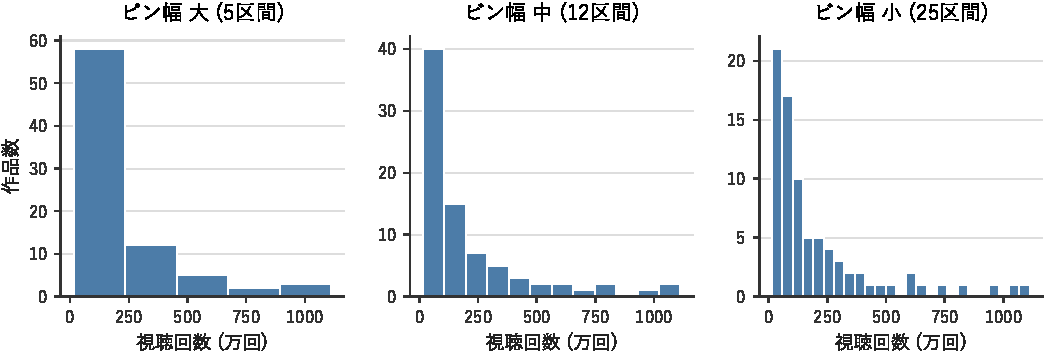
\includegraphics[width=\linewidth]{../figures/output/ch03_histogram.pdf}
        \caption{80本の視聴回数のヒストグラム. 階級の幅を3通りに変えて表示. 縦軸の目盛りは図ごとに異なる.}
        \label{fig:ch03_histogram}
      \end{figure}

      まず, 視聴回数の散らばり方を見るために, ヒストグラムを描く.
      階級の幅を3通り (大・中・小) に変えた図を並べ, 幅を変えても変わらない特徴を確かめる.
      なお, 縦軸 (映画の本数) の目盛りは図ごとに別々なので, 図どうしで棒の高さを直接比べることはできない. 比べるのは分布の形だけだ.

      どの幅で描いても, 視聴回数の少ない側に山があり, 多い側に長く裾を引いている.
      視聴回数の少ない映画が大半で, 右端には視聴回数が桁違いに大きい映画が少数ある.

      前章では, 視聴回数の平均が $209.4$ 万回, 中央値が $107.1$ 万回で, 平均が中央値の約2倍まで膨らんでいた.
      平均をここまで押し上げる映画が, 視聴回数の多い側にあるはずだと推測はできたが, 数値だけでは分布の形までは確かめられなかった.
      ヒストグラムを見ると, 右に裾を引いていることが確認できる.

      この右に裾を引く形は, 80本をひとまとめにして見たときの形だ.
      ジャンルごとに分けたとき, どのジャンルにも同じ形が現れるのか, それともジャンルによって様子が違うのかは, 全体のヒストグラム1枚からは分からない.
      次は, ジャンルで分けて視聴回数を見る.

    \subsubsection*{2枚目: ジャンル別視聴回数の箱ひげ図}

      \begin{figure}[htbp]
        \centering
        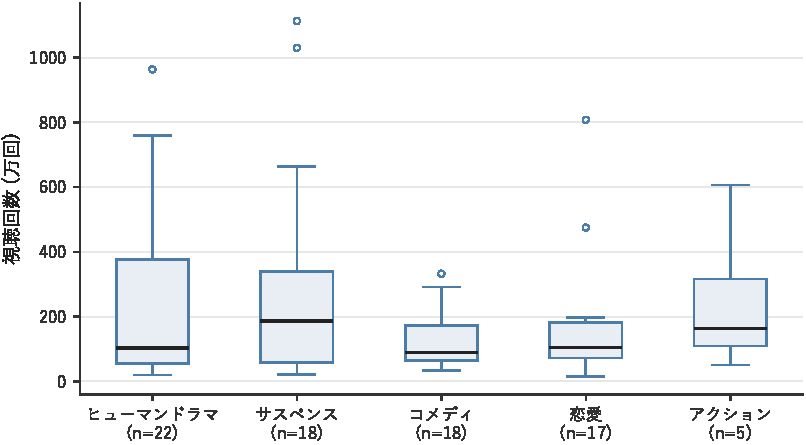
\includegraphics[width=0.85\linewidth]{../figures/output/ch03_boxplot.pdf}
        \caption{ジャンル別（ヒューマンドラマ・サスペンス・コメディ・恋愛・アクション）の視聴回数の箱ひげ図. 各ジャンルの件数を併記.}
        \label{fig:ch03_boxplot}
      \end{figure}

      80本の映画はいくつかのジャンルに分かれている.
      ジャンルごとの視聴回数を比べるために, 横軸にジャンル, 縦軸に視聴回数をとって箱ひげ図を並べる.

      ジャンルによって箱の位置（中央値）が違う.
      箱の高さ（四分位範囲）もジャンルごとに違っていて, 中央値の近くにまとまっているジャンルもあれば, 縦に大きく広がっているジャンルもある.
      ひげの外側にある点（外れ値）の出方も, ジャンルによって違う.
      ジャンルによって, 視聴回数の典型値や散らばりに違いがありそうだ.

      ただし, 同じジャンルの中に, よく見られた映画とあまり見られなかった映画がはっきり分かれて混じっていたとしても, 箱ひげ図の上では見分けがつかない.
      気になるジャンルがあれば, そのジャンルだけヒストグラムを描いて確かめる.

      ジャンルによって視聴回数の典型値や散らばりが違うなら, 視聴回数と一緒に動いている量がほかにもありそうだ.
      手元のデータでまず思い当たるのは製作費だ.
      製作費と視聴回数の関係を, 散布図で見る.

    \subsubsection*{3枚目: 製作費と視聴回数の散布図}

      \begin{figure}[htbp]
        \centering
        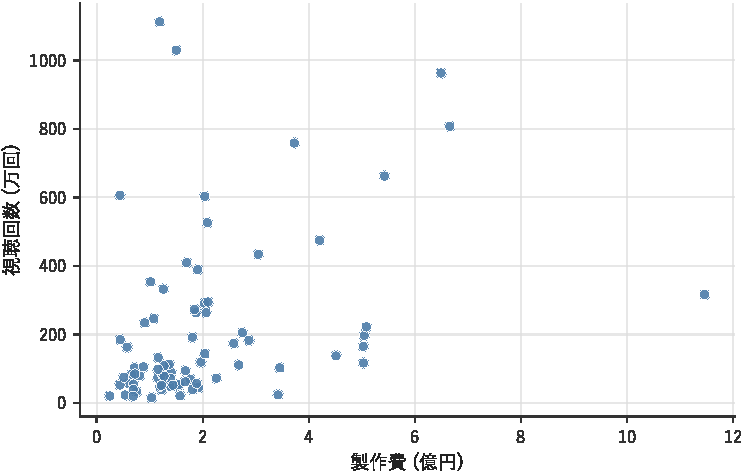
\includegraphics[width=0.8\linewidth]{../figures/output/ch03_scatter.pdf}
        \caption{横軸が製作費 (億円), 縦軸が視聴回数 (万回) の散布図.}
        \label{fig:ch03_scatter}
      \end{figure}

      横軸に製作費, 縦軸に視聴回数をとり, 各映画を点で表す.
      点の並びには, 全体として右肩上がりの傾向が見える.
      製作費が大きい映画ほど, 視聴回数も多い傾向がある.
      ただし関係はきれいな直線ではなく, 製作費が同じくらいの映画どうしでも視聴回数には大きな散らばりがある.

      それでも, この図から言えるのは「正の相関がありそうだ」までで, 「製作費を増やせば視聴回数が増える」とまでは言えない.
      製作費が視聴回数を引き上げているのか, 話題性や宣伝の規模といった別の要因が両方に関係しているだけなのかは, 散布図からは判別できないからだ.

    \subsubsection*{3枚の図から見えたこと}

      視聴回数の全体は右に裾の長い分布で, ジャンルごとに見れば典型値も散らばりも違い, 製作費とのあいだには正の相関がありそうだった.
      1枚目で気づいた形のかたよりが, ジャンルで分ける2枚目につながり, 2枚目で見えた群ごとの違いが, 製作費を横軸にとる3枚目につながった.
      図を描いて気づき, 気づいたことを次の図で確かめる往復を, ここで一巡したことになる.

      この往復で手に入ったのは, 確定した結論ではなく, 次に検証したい仮説だ.
      ジャンル間の差は, 偶然の範囲を超えているのか.
      製作費と視聴回数の関係は, どのくらい強いと言ってよいのか.
      答えるには, 図を眺めるのとは別の方法が必要になる.


  \subsection{結果と次の一手}

    この章では, 統計量だけでは見えにくかったデータの形を, 図にして確かめてきた.
    ヒストグラムで散らばりの形を, 箱ひげ図で群ごとの違いを, 散布図で量どうしの関係を見た.
    見たいことが違えば, 描く図も違う.

    ただし, この章で読み取ったことは, 手元の80本についての結果でしかない.
    別の80本を取り直したら, 視聴回数は同じように右に裾を引くだろうか.
    ジャンルによる差は同じように出るだろうか.
    製作費と視聴回数の関係は同じくらい強いだろうか.
    取り直すたびに同じ結果になるとは限らない.

    取り直したときに結果がどう変わるかが分からないと, 図から読み取ったことが手元の80本にだけ当てはまるのか, それとも背後にある集まりの性質を映しているのかを区別できない.
    次章では, 取り直したときに結果がどれだけばらつくかを見積もる方法を考えていく.


\newpage

\section{確率分布と中心極限定理 : 推論の足場をつくる}

  \subsection{問い}

    前章では, 数字の羅列を図にして, データの形を見た.
    80本の映画の視聴回数は, 少ない側に山があり, 多い側へ長く裾を引いていた.
    ジャンルごとに典型値や散らばりの様子も違っていた.

    ただ, 前章の終わりにひとつ問いが残っていた.
    この形は, 手元の80本だけのものなのだろうか.
    別の80本を選び直しても, やはり同じように右へ裾を引くのだろうか.
    取り直したときに結果がどれだけ変わりうるのかが分からないと, 図から読み取ったことがどこまで信用できるのか, 判断のしようがない.

    もっとも, 「取り直しても同じ形か」と問うには, その前に, いま見えている形が言葉で言えていなければならない.
    取り直した結果と見比べて同じか違うかを言うには, 元の形の記述が要るからだ.
    そこでまず, 手元の80本の形を言葉にするところから始める.

  \subsection{素朴な方法と限界}

    形を言葉にするだけなら, 難しいことは何もないように思える.
    前章でも「右に裾が長い」「山は一つ」と書き留めてきたし, それで十分伝わっているようにも思える.
    ためしに手元の80本について, 製作費と評価件数のヒストグラムを\cref{fig:ch04-hist-compare}のように並べてみる.

    \begin{figure}[htbp]
      \centering
      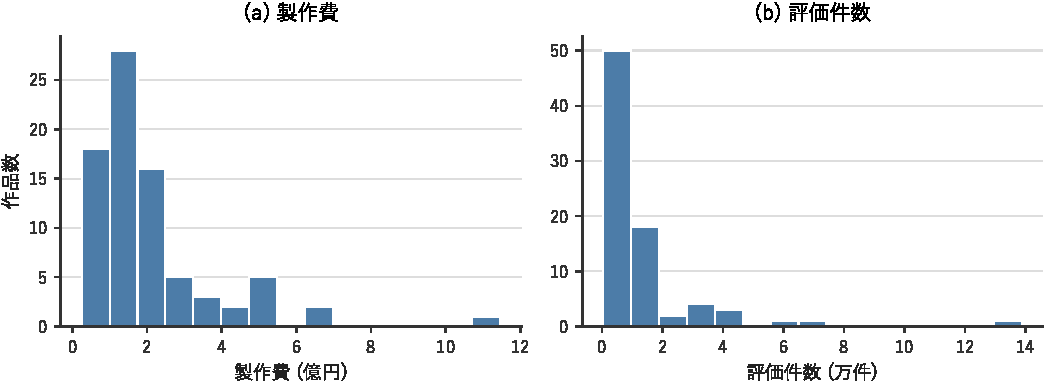
\includegraphics[width=\linewidth]{../figures/output/ch04_hist_compare.pdf}
      \caption{80本の製作費と評価件数のヒストグラム. どちらも右に裾が長いが, 評価件数は少数の作品がとくに大きな値をとる.}
      \label{fig:ch04-hist-compare}
    \end{figure}

    どちらも右に裾が長い.
    しかし並べて見れば, 歪みの程度はまるで違う.
    製作費は, 山のまわりに大半の作品が収まっていて, 裾は緩やかに伸びる程度だ.
    評価件数のほうは, 少数の作品が桁違いに大きく, 裾が横へ長く引き延ばされている.
    「右に裾が長い」という同じひとことに, この二つが同居してしまう.

    そこで, 「かなり長い」「やや長い」と程度を添えてみる.
    ところが, どこからが「かなり」なのかは人によって違う.
    同じ図を見て, ある人は「強く歪んでいる」と言い, 別の人は「少し偏っているだけ」と言うかもしれない.
    程度を測る共通の物差しがないのだ.

    しかも, かりにうまい物差しが見つかったとしても, それで測れるのは手元の80本の形までだ.
    どれほど正確に形容しても今回の標本の描写でしかなく, 「この形は偶然か, それとも仕組みか」を判断する基準は, データの中をいくら見つめても出てこない.

    そうなると, 基準は手元のデータの外に置くしかなさそうだ.
    データの値は, 何もないところから現れたわけではなく, 何かの仕組みから生まれている.
    その仕組みの側から, 形を考えてみる.

  \subsection{理論の最小核}

    \subsubsection*{理論分布 : 仕組みの側から決まる形}

    確率パートで, サイコロの目やコインの表裏を確率変数として扱った.
    サイコロを振る前から, どの目がどれくらい出やすいかは決まっていて, その出やすさの全体を書き表したものが確率分布だった.
    つまり確率分布は, 出た値を集計して得られるものではない.
    値を生む仕組みの側に, はじめから備わっている.

    この見方を, 手元のデータに向けてみよう.
    映画の視聴回数も, 何かの仕組みから生まれた値だと考えられる.
    作品の魅力, 宣伝の規模, 公開のタイミング.
    いろいろな要因が絡み合った結果として, 一本ごとの値が決まっている.
    その仕組みのすべてを書き下すことはできない.
    しかし, もし仕組みのあらましを確率分布のかたちで表せたなら, その分布の形は, 階級の幅にも, どの80本を引き当てたかにも左右されない.
    手元のヒストグラムは, その理論上の形に, 標本ごとの偶然のでこぼこが乗ったものと見なせる.

    このように, データの形の基準として使う確率分布を, \textbf{理論分布}と呼ぶ.
    中身は確率パートで学んだ確率分布そのものであり, 新しい数学が増えるわけではない.
    変わるのは使い方だ.
    確率パートではサイコロのように仕組みが分かっている前提で値の出方を考えたが, ここでは逆に, 目の前のデータの背後にどんな仕組みがありそうかを考えるために使う.

    名前のついた理論分布は, 数えるほどしかない.
    世の中のデータは無数にあるのに, なぜそれで足りるのか.
    それは, 値を生む仕組みのほうに, 共通の骨組みが繰り返し現れるからだ.
    成功か失敗かを何回も数え上げる.
    めったに起きない出来事の回数を数える.
    小さな要因がたくさん足し合わさる.
    こうしたよくある骨組みの一つひとつに, 対応する形が一つずつ付いている.
    分布の名前は, いわば仕組みの名前なのだ.
    代表的な対応は章末のコラム「仕組みから見る理論分布」にまとめたので, 全部を暗記する必要はない.

    そうなると, やることは決まったように見える.
    名前のついた分布の中から手元のデータに合う形を探し当てて, 「視聴回数は〇〇分布に従う」と言えばよい.
    そう言えてしまえば, あとはその分布の性質を使って, 取り直したときに何が起きるかまで計算できそうだ.

    ところが, この道は見かけほど通れない.
    理論分布は, 仕組みを単純化して取り出した理想の形である.
    一方, 視聴回数の背後にあるのは, 書き下すこともできないほど込み入った仕組みだった.
    そんな仕組みから生まれた値が, どれかの理想の形にぴったり従ってくれることは, まずない.
    しかも, かりにぴったり従っていたとしても, 手元にあるのは80本の標本だけで, それを確かめきる手段がない.
    「データは〇〇分布に従う」は, どこまでいっても人間の側の見立てである.
    見立ての上に推論を積めば, 見立てが外れたとき, 積んだ結論ごと崩れる.

    それでも, 見立てがまったくの無駄になるわけではない.
    ぴったりの一致を求めるのをやめて, ヒストグラムと形を見比べ, いま知りたいことに差し支えない程度に近ければ「近い」と言う.
    たとえば「評価件数の分布は対数正規分布に近い」と言えたとする.
    対数正規分布は, たくさんの要因の掛け算が生む, 右に長い裾をもつ理論分布だ(コラム参照).
    この一言で, 聞き手は歪みの程度まで含めて同じ形を思い浮かべられるし, 背後の仕組みについて「掛け算の積み重ねだろうか」という見当まで持てる.
    「右に裾が長い」という感覚頼みの形容が, 基準のある記述に変わる.
    形を語る共通の言葉としてなら, 理論分布は十分に役に立つ.

    ただし, 言葉として役に立つことと, 推論の土台になることは別だ.
    「近い」はあくまで見立てで, その上に「取り直したらどうなるか」の答えを積むわけにはいかない.
    この行き詰まりには抜け方がある.
    ただ, そのためには, 理論分布を一つだけ, 性質までよく知っておく必要がある.
    正規分布だ.

    \subsubsection*{正規分布 : 足し算が生む釣鐘型}

    \textbf{正規分布}は, 左右対称の釣鐘型をした理論分布で, 対応する仕組みは「多数の小さな要因の足し算」である.
    この仕組みが現実にありふれているために, 正規分布はいろいろな場面で繰り返し現れる.

    たとえば人の身長を考えてみる.
    遺伝, 栄養, 運動, 睡眠と, 多数の要因がそれぞれ少しずつ影響して, その積み重ねとして身長が決まる.
    どれか一つの要因が全体を支配することはない.
    こういう成り立ちの量を大勢の人から集めると, 分布は釣鐘型に近づくことが知られている.
    釘を並べた板の上からボールを落とす装置(ゴルトンボード)でも同じことが起きる.
    ボールは釘に当たるたびに左右のどちらかへ小さく逸れ, 着地点は逸れの合計で決まる.
    ボールをたくさん落とすと, 着地点の分布は釣鐘型になる.
    小さなランダムな逸れの足し算, という骨組みが共通しているからだ.

    この釣鐘型を数式で書いたものが, 次の正規分布である.

\begin{defi}{正規分布}{normal_dist}
  確率変数 $X$ が平均 $\mu$, 分散 $\sigma^2$ の\textbf{正規分布}に従うとき, $X \sim N(\mu, \sigma^2)$ と書く.
  その確率密度関数は
  \[
    f(x) = \frac{1}{\sqrt{2\pi\sigma^2}} \exp\!\left( -\frac{(x - \mu)^2}{2\sigma^2} \right)
  \]
  で与えられる.
\end{defi}

    式は見た目より素直にできている.
    まず $(x - \mu)^2$ は, 平均からの距離の二乗だ.
    それがマイナス符号つきで指数関数に入っているから, 平均から離れるほど $f(x)$ は急速に小さくなる.
    つまり, 平均の近くの値ほど出やすく, 遠い値ほど出にくい.
    次に分母の $\sigma$ を見ると, $\sigma$ が大きいほど $(x-\mu)^2$ を割る $2\sigma^2$ が大きくなり, 減り方が緩やかになる.
    山が低く, 裾の広い形になるわけだ.
    逆に $\sigma$ が小さければ, 中心に集中したとがった形になる.
    どこを中心に($\mu$), どれくらいの幅で($\sigma$)散らばるか.
    この2つの数だけで, 正規分布の形は完全に決まる.

    \begin{figure}[htbp]
      \centering
      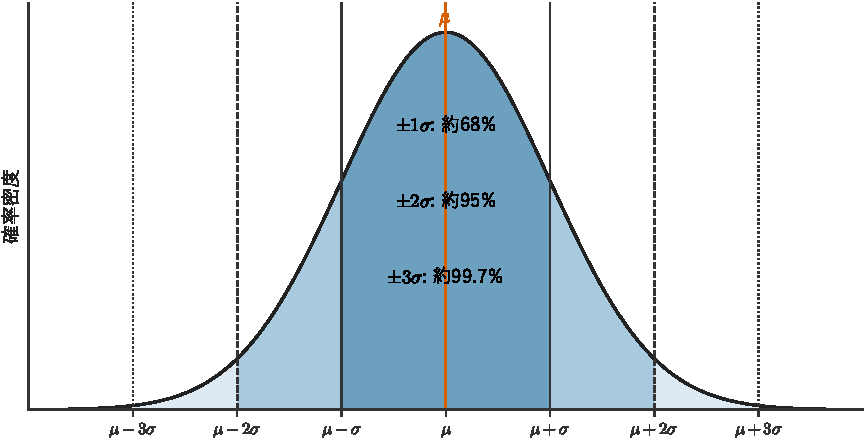
\includegraphics[width=0.9\linewidth]{../figures/output/ch04_normal_ranges.pdf}
      \caption{正規分布で平均から $\pm1\sigma$, $\pm2\sigma$, $\pm3\sigma$ に収まる範囲. 線種と濃淡の両方で境界を示した.}
      \label{fig:ch04-normal-ranges}
    \end{figure}

    形が2つの数で決まるおかげで, 値がどの範囲に散らばるかも, この2つから読み取れる.
    正規分布では, 平均から $\pm 1\sigma$ の範囲に全体の約68\%, $\pm 2\sigma$ に約95\%, $\pm 3\sigma$ に約99.7\%が収まる.
    この割合は $\mu$ や $\sigma$ の値によらず, いつでも同じだ.
    だから, データが正規分布に近いと言えたら, 平均と標準偏差の2つの数を報告するだけで, 聞き手は「値のほとんどがどの範囲にあるか」まで再現できる.
    第2章で学んだ平均と標準偏差は, 分布の形が釣鐘型に近いとき, 数ある要約の中でも特に多くの情報を伝える.
    製造業の品質管理で「寸法が $\pm 3\sigma$ に収まれば合格」という基準が使われてきたのも, この性質をそのまま規格にしたものだ.

    \subsubsection*{取り直したときの平均のばらつき}

    ここで手元のデータに目を戻すと, 少し具合が悪い.
    視聴回数のヒストグラムは右へ大きく歪んでいて, 釣鐘型にはほど遠い.
    実際のところ, 視聴回数, 年収, 評価件数と, 世の中のデータにはむしろ歪んだ形のほうが目につく.
    行き詰まりを抜けるどころか, 正規分布もまた, 手元のデータには当てはまらない理論分布の一つにしか見えない.

    それでも正規分布には出番がある.
    ただし, データそのものの形としてではない.
    それを確かめるために, 前章から持ち越している「取り直したらどうなるか」という問いを, 小さな例で考えてみる.

    ある商品のレビュー評価の平均を知りたいとする.
    レビューは全部で1000件あって, もちろんこの全てを確認できればいいのだが, 残念ながら手元には全体のうち50件しかないとしよう.
    そして, その50件の平均を計算してみると4.2だった.
    では, この計算を基にレビュー全体の平均も4.2と言っていいだろうか.
    もっと言うと, もう一度別の50件を取っても, 平均は再び4.2になるだろうか.
    おそらくそうはならないだろう.
    レビュー全体の平均は4.2とは限らないし, 別の50件を取り直してみたら今度は4.0かもしれない.
    標本を取り直すたびに, 平均は毎回少しずつ違う値になってしまう.

    この事実は当たり前に思えるが, かなり厄介だ.
    手元の4.2という数字が, 本当の平均(母集団の平均なので\textbf{母平均}と呼ぶ)からどれくらい離れているのか分からないからだ.
    1回しか観測していないのに, 「取り直したら毎回違う」という性質にどう対処するのか.
    本章と次章で, この問題にある程度もっともらしい対処法を示していく.

    肝になるのは, 「もし何度も取り直したら, 平均はどんなふうに分布するのか」を考えてみることだ.
    1回ごとの平均の値は予測できなくても, 何度も取り直したときの散らばり方には, 決まったパターンがありうる.
    散らばり方が分かれば, 手元の1回の結果が母平均からどれくらい離れうるのかを見積もる足がかりになる.

    このように, 標本を取り直すたびに統計量を計算し直したとき, その統計量の値が従う分布を\textbf{標本分布}と呼ぶ.

\begin{defi}{標本分布}{sampling_dist}
  母集団から標本を繰り返し取り直し, そのたびに統計量を計算するとき, その統計量の値が従う確率分布を, その統計量の\textbf{標本分布}と呼ぶ.
\end{defi}

    名前がまぎらわしいので, 先に注意しておきたい.
    標本分布は, 手元の標本そのものの分布ではない.
    50件のレビューの星の値がどう散らばっているか, という話なら, それは手元のデータの分布であって, 前章までに見てきたヒストグラムの世界だ.
    標本分布はそうではなく, 「平均」という一つの統計量を, 取り直しのたびに計算し直したとき, その平均の値がどう散らばるか, という分布である.
    データの分布は目の前に描けるが, 標本分布は「もし取り直したら」という仮想の繰り返しを考えて初めて定まる.
    見ている対象がまるで違うので, 混同しないようにしたい.

    ただ, こう定義してみると, 事態は前より苦しくなった気さえする.
    データの分布なら, 少なくともヒストグラムに描いて眺めることはできた.
    標本分布は仮想の繰り返しの上にしか存在しないから, 一度も目に見えない.
    見えるデータの分布でさえ, 理論分布への当てはめは見立ての域を出なかった.
    見えない分布の形など, どうやって知ればよいのか.

    \subsubsection*{中心極限定理 : 平均のばらつきは釣鐘型になる}

    幸い, サイコロのように仕組みを完全に決められる例なら, 「取り直しては平均を計算する」という繰り返しを, 実際にやってみせられる.
    元のデータが歪んでいれば, 平均の散らばり方も同じように歪むと考えるのが自然な気がする.
    それも確かめたいので, わざと偏った例で実験してみよう.

    1の目が出る確率だけが50\%で, 2から6の目は各10\%という, 極端に偏ったサイコロを考える.
    このサイコロを5回振って, 出た目の平均を記録する.
    この「5回振って平均を取る」をまるごと1000回繰り返し, 記録された1000個の平均をヒストグラムにする.

    \begin{figure}[htbp]
      \centering
      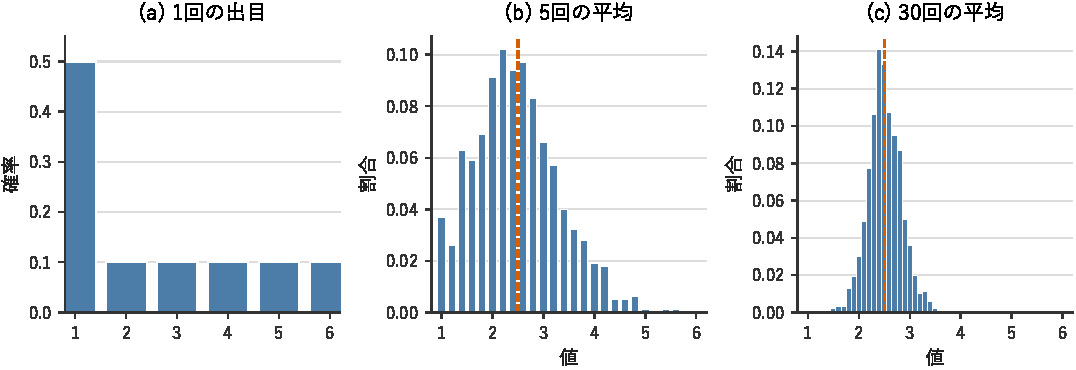
\includegraphics[width=\linewidth]{../figures/output/ch04_dice_clt.pdf}
      \caption{偏ったサイコロの出目と標本平均の分布. 破線は理論上の平均2.5. 5回または30回振って平均を取る操作を1000回ずつ繰り返した. 5回の平均は0.2刻みの値しか取らないため, (b)の棒は櫛状に並ぶ.}
      \label{fig:ch04-dice-clt}
    \end{figure}

    \cref{fig:ch04-dice-clt}を見ると, 5回振りの平均のヒストグラムは, 元のサイコロほどではないにせよ, まだ右に裾を引いた形をしている.
    ところが, 5回を30回に増やして同じことをすると, 平均のヒストグラムはかなりきれいな釣鐘型になる.
    元の分布はどう見ても釣鐘型ではないのに, 平均の散らばり方のほうは左右対称の釣鐘型に近づいていく.
    偶然ではなく, 次の定理が成り立っているためだ.

\begin{thm}{中心極限定理}{clt}
  平均 $\mu$, 分散 $\sigma^2$ をもつ同一の分布から, 互いに独立に $n$ 個の値を取り出し, その標本平均 $\bar{X}$ を計算する.
  $n$ が大きくなるにつれて, $\bar{X}$ の標本分布は正規分布 $N\!\left(\mu,\; \sigma^2 / n\right)$ に近づく.
\end{thm}

    定理の中身を, 部品ごとに確認していく.

    まず前提は, 「同一の分布から, 互いに独立に」の一つだけだ.
    各値が同じ仕組みから生まれていて, ある値の出方が別の値の出方に影響しない, という条件である.
    統計学ではこの条件を\textbf{独立同分布}(i.i.d.: independent and identically distributed)と呼ぶ.
    サイコロの実験なら, 毎回同じサイコロを, 前の結果と関係なく振っていることに当たる.

    次に, 元の分布の形については何も要求していない.
    歪んでいても, 平坦でも, 山が二つあってもよい.
    元のデータがどの理論分布に従うのかを, 見立てる必要すらない.
    i.i.d.でありさえすれば, 平均の標本分布は正規分布へ近づいていく.
    偏ったサイコロの実験で見たのは, まさにこの働きだ.

    「$n$ が大きくなるにつれて」という部分は, 前提条件ではなく, 近づく速さの話である.
    $n$ がいくつ以上なら使ってよい, という境目があるわけではなく, $n$ が増えるほど近似がよくなっていく.
    ただし近づく速さは元の分布の形に左右される.
    元の分布が対称に近ければ $n = 10$ 程度でもかなり釣鐘型に近づくし, 強く歪んでいれば $n = 30$ や $50$ でもまだ歪みが残ることがある.
    「$n \geq 30$ なら大丈夫」という目安を見かけることがあるが, 保証ではなく目安にすぎない.
    元のデータのヒストグラムを見て, 歪みが強いほど $n$ に余裕を見る, というのが実務的な使い方になる.

    そして, 近づく先が $N(\mu,\; \sigma^2/n)$ である.
    中心は元の分布の平均 $\mu$ のままで, 分散が $\sigma^2/n$ に縮んでいる.
    $n$ が大きいほど, 平均の散らばりは小さくなる.
    5件の平均より100件の平均のほうが, 取り直しても安定するはずだという直感と合っている.

    視聴回数のように歪んだデータでは, 正規分布はデータの形の記述としては出番がなかった.
    しかし, そのデータから計算した平均が取り直しでどうばらつくかを考えると, そこには正規分布が現れる.
    それも元の形を問わずに現れるのだから, データが釣鐘型かどうかを心配する必要すらない.

    振り返ると, この章には性格のまるで違う分布が二つ出てきたことになる.
    一つは, データの背後に見立てる理論分布だ.
    「評価件数は対数正規分布に近い」というときの分布で, これは人間の側の見立てであり, 当たっている保証はどこにもなかった.
    もう一つは, 平均という統計量が従う分布だ.
    こちらは見立てではない.
    i.i.d.という前提のもとで, 元のデータがどんな分布だろうと正規分布に近づくことが, 定理として保証されている.
    この後の章で組み立てていく推論は, 「データは〇〇分布に従うはずだ」という当てにならない見立てにではなく, この保証の上に立つ.
    正規分布が統計学の中心に置かれているのも, 釣鐘型のデータが多いからではなく, 統計量のばらつき方というこの土台の側に現れるからだ.

    なお, i.i.d.が崩れている場合, たとえばデータどうしが連動している場合には, この定理はそのままでは使えない.
    そうしたデータへの対処法も研究されているが, 本書ではi.i.d.が成り立つ場合を扱う.

    \subsubsection*{標準誤差 : ばらつきの幅を一つの数にする}

    前の節で見たとおり, 平均の標本分布は正規分布 $N(\mu,\; \sigma^2/n)$ に近づく.
    正規分布の形は, 中心と幅の2つの数で決まるのだった.
    中心は母平均 $\mu$ だから, 残る知りたい量は幅, つまりこの分布の標準偏差である.
    分散が $\sigma^2/n$ なので, 標準偏差はその平方根の $\sigma/\sqrt{n}$ になる.
    取り直したときの平均のばらつきの幅が, この一つの数に集約されている.
    そこで, この量に名前を付ける.

    ただし, 母集団の標準偏差 $\sigma$ は手元から直接は分からない.
    そこで推論では, 手元の標本から
    \[
      u^2 = \frac{1}{n-1}\sum_{i=1}^{n}(x_i-\bar{x})^2, \qquad u = \sqrt{u^2}
    \]
    を計算し, $u$ で $\sigma$ を見積もる.
    $u^2$ は\textbf{不偏分散}, $u$ はその平方根である.
    第2章の $s^2$ は手元のデータを記述するために $n$ で割った量であり, 目的が違う.
    同じデータから計算しても値が少し異なるのは, 第2章の定義が誤りだったからではない.
    なぜ推論では $n-1$ で割るのかは, 検定の数学的背景を扱う章で確かめる.

\begin{defi}{標準誤差}{se}
  母集団の標準偏差を $\sigma$, 標本サイズを $n$ とするとき, 標本平均の\textbf{標準誤差}(SE: Standard Error)を
  \[
    \mathrm{SE} = \frac{\sigma}{\sqrt{n}}
  \]
  と定義する.
  実際には $\sigma$ は未知であるため, 推論用標準偏差 $u$ で置き換えた $\mathrm{SE} = u / \sqrt{n}$ を用いる.
\end{defi}

    定義の後半に断りが入っているのは, $\sigma$ が母集団の値であって, 手元からは分からないためだ.
    その代わりに, 手元の標本から計算した $u$ を使う.
    標本がそこそこ大きければ $u$ は $\sigma$ の代用として使えるので, 本書では以降, $\mathrm{SE} = u/\sqrt{n}$ を標準誤差として使っていく.
    $n$ が小さいときには別に補正のしかたが知られているが, 本書ではデータ数がそこそこ多い場合を扱う.

    式の部品は2つしかない.
    分子の $u$ は, データそのものの散らばりの大きさを推論用に計算した値だ.
    個々の値が大きく散らばるデータほど, 平均も取り直しのたびに大きく動く.
    分母の $\sqrt{n}$ は, 標本サイズの平方根だ.
    件数が多いほど平均は安定する.
    ただし $n$ がそのままではなく $\sqrt{n}$ で効くので, SEを半分にしたければ $n$ は4倍必要になる.
    データを増やせば平均の精度は上がるが, 件数に比例してどこまでも上がるわけではない, ということもこの式から読み取れる.

    名前も式も標準偏差(SD)とよく似ているので, 区別をはっきりさせておこう.
    SDは, 個々のデータが平均のまわりにどれくらい散らばっているかを表す.
    第2章から使ってきた, データの散らばりの指標だ.
    一方SEは, 平均という統計量が, 標本の取り直しに対してどれくらいばらつくかを表す.
    測っている対象が, 個々のデータと統計量とでまるで違う.
    $n$ が大きくなってもSDはほぼ一定のままだが, SEは $\sqrt{n}$ に反比例して小さくなっていく, という振る舞いの違いにも, 対象の違いが表れている.

    「取り直したら結果はどれだけばらつくのか」という冒頭からの問いに, 平均についてはこう答えられる.
    ばらつきの形は正規分布に近づき, 幅は $u/\sqrt{n}$ という一行の計算で見積もれる.
    実際に取り直しを繰り返す必要はなく, 手元の標本が1組あれば計算できる.

  \subsection{手法}

    \subsubsection*{前提条件}
    \begin{itemize}
      \item 観測値が独立同分布(i.i.d.)であること. すなわち, 各観測値が同じ仕組みから生まれ, 互いに影響しないこと.
    \end{itemize}

    前提はこの1点である.
    「$n$ が大きいこと」は前提には入れていない.
    $n$ の大きさが左右するのは正規分布への近さ, つまり近似の精度であって, 手順が使えるかどうかの境目ではないからだ.
    元のデータの歪みが強いほど, 近似の精度には余裕を見ておく.

    \subsubsection*{手順}

    \textbf{Step 1. 形を確認する.}
    ヒストグラムを描き, 山の数, 対称性, 裾の長さ, 外れ値の有無を見る.
    章末のコラムの対応を手がかりに, 近そうな理論分布があれば見当を付けておく.
    強い歪みや極端な外れ値があれば, $n$ とのバランスで正規近似の精度が粗くなることを頭に入れておく.

    \textbf{Step 2. 平均 $\bar{x}$, 推論用標準偏差 $u$, 件数 $n$ を確認する.}
    平均と件数に加え, $n-1$ で割る不偏分散から $u$ を計算する.

    \textbf{Step 3. SEを計算する.}
    \[
      \mathrm{SE} = \frac{u}{\sqrt{n}}
    \]
    これで, 平均を取り直したときのばらつきの幅が見積もれた.

    報告や記録には, 平均とあわせてSEと $n$ を書き添える.
    このときSDとSEを取り違えないよう注意する.
    データそのものの散らばりを伝えたいならSD, 平均がどれだけ安定して求まっているかを伝えたいならSEであり, 両方書くのが親切だ.

  \subsection{実践}

    ランニング例に戻ろう.
    手元にあるのは, 配信サービスの対象作品から抽出された80本の視聴回数だった.
    まず, 中心極限定理が実際に成り立つ様子を確かめ, そのあと手元の平均のSEを計算する.

    \subsubsection*{平均の散らばりを目で見る}

    手元の80本は, サービス全体の対象作品の一部だった.
    もし同じような調査をもう一度行えたら, 平均視聴回数は今回と同じ値になるだろうか.
    実際に調査を何度もやり直すことはできないが, その様子に近いものなら, 手元の80本を使った実験で再現できる.
    まず, 80本のどれも同じ確率で選ばれる仮の分布を作り, 対象作品全体の代わりに使う.
    本数を増やすと平均の散らばりがどう変わるかをあとで見比べるため, まずは少なめの20本で試す.
    この仮の分布から20本を選ぶときは, 一度選んだ作品も候補に戻してから次を選ぶ.
    そのため, 1回の中で同じ作品が複数回選ばれることもある.
    この選び方を\textbf{復元抽出}と呼ぶ.
    20本の平均を計算する操作を1000回繰り返し, 1000個の平均をヒストグラムにする.

    ただし, この実験はサービス全体から20本を本当に取り直す操作と同じではない.
    手元の80本を母集団の代役にした近似であり, 80本の抽出に偏りがあれば, その偏りも引き継ぐ.

    \begin{figure}[htbp]
      \centering
      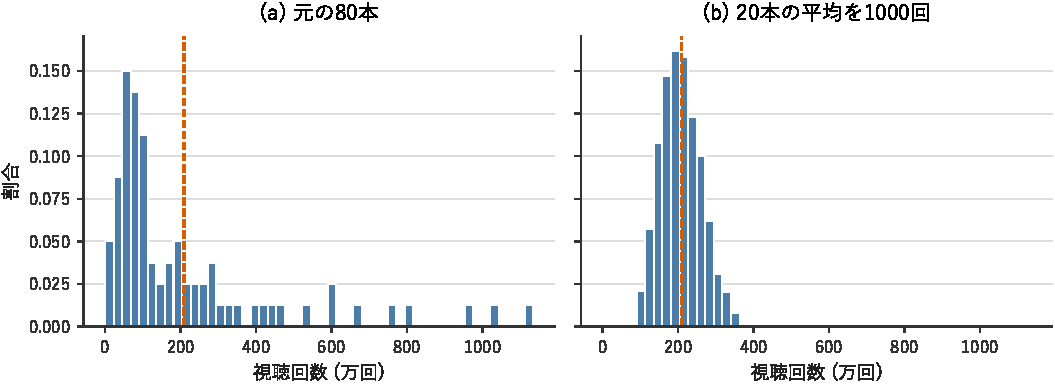
\includegraphics[width=\linewidth]{../figures/output/ch04_sampling_dist.pdf}
      \caption{元の80本の視聴回数と, 80本から20本を復元抽出して求めた標本平均の分布. 復元抽出と平均の計算を1000回繰り返した. 横軸と縦軸の尺度は左右で共通で, 破線は80本の平均を示す.}
      \label{fig:ch04-sampling-dist}
    \end{figure}

    \cref{fig:ch04-sampling-dist}の左側にある元の視聴回数の分布は, これまで見てきたとおり右へ大きく歪んでいる.
    ところが, 20本ずつの平均のヒストグラムは, 左右対称の釣鐘型にかなり近い.
    しかも, 散らばりの幅は元のデータよりずっと狭い.
    歪んだデータからでも, 平均の散らばり方は釣鐘型になる.
    前の節で定理として確認したことが, 手元の80本を使った実験にも表れている.

    \subsubsection*{80本の平均にSEを添える}

    実験で見たのは, 20本ずつ選んだときの平均の散らばりだった.
    一方, 実際に手元にあるのは80本の標本が1組であり, 知りたいのはこの80本の平均のばらつきである.
    件数が違うからといって, 実験を組み直す必要はない.
    SEの式は $n$ の値に応じて幅を見積もれるから, $n = 80$ を入れればよい.
    件数が20本の4倍あるので, $\sqrt{n}$ の働きにより, 幅は実験で見た散らばりのおよそ半分になるはずだ.

    実際に計算してみよう.
    80本の視聴回数について, 平均 $\bar{x}$ はおよそ $209.4$ 万回だった.
    同じ80本から推論用標準偏差 $u$ を計算すると, およそ $240.8$ 万回となる.
    件数は $n = 80$ なので, SEは
    \[
      \mathrm{SE} = \frac{u}{\sqrt{80}} \approx \frac{240.785}{8.944} \approx 26.921
    \]
    となり, およそ $26.9$ 万回になる.

    この数字の読み方を確認しておこう.
    SDである $u$ は, 一本一本の作品の視聴回数がどれだけ散らばっているかを推論用に見積もった値である.
    一方SEは, もし同じ条件で80本の調査を取り直したら, 平均がどの程度動きうるか, という見積もりだ.
    $\sqrt{80} \approx 8.9$ で割っているから, SEはSDの9分の1ほどしかない.
    一本一本の値は大きくばらつくのに, 80本まとめた平均はその何分の一かの幅にしか散らばらない.
    平均という統計量の安定ぶりが, この2つの数字の開きに表れている.

    ただし, この見積もりが頼れるのは, 80本がi.i.d.に近い状況で選ばれている場合だ.
    第1章で置いた「この80本を対象作品全体から大きな偏りなく抽出された標本として扱う」という仮定が, ここで効いている.
    もし抽出に偏りがあれば, SEがいくら小さくても, 平均そのものが母平均からずれた場所に集まってしまう.
    SEが見積もるのは取り直しによるばらつきであって, 偏りの大きさではない.

  \subsection{結果と次の一手}

    出発点は, 「手元で見えた形は, 取り直しても残るのか」という問いだった.
    形を感覚に頼らず語るために理論分布を導入すると, 形の背後にある仕組みごと語れる共通の言葉にはなった.
    しかし, 現実のデータがどれかの理論分布にぴったり従うことは期待できず, 「データは〇〇分布に従う」という見立てを推論の土台にはできなかった.

    突破口は, 問う相手をデータの分布から統計量の分布に替えたことだった.
    手元のデータが歪んでいても, 平均を取り直したときの散らばり方は, i.i.d.のもとで正規分布に近づく.
    これは見立てではなく中心極限定理が保証する事実であり, その散らばりの幅が標準誤差 $\mathrm{SE} = u/\sqrt{n}$ だった.
    手元の標本1組から, 「取り直したら平均はこの程度動きうる」という見積もりが一行の計算で出せる.
    前章まで, 手元の80本について言えることは80本の中で閉じていた.
    いまは, 取り直したらどうなるかという手元の外側への見通しが, 初めて数字になっている.

    ただ, 実際の報告の場面を考えると, もう一歩足りない.
    「平均はおよそ何回, SEはおよそ何回」と伝えられた相手は, その平均をどこまで信用してよいのか, まだ読み取りにくい.
    足りないのは, SEという散らばりの目安を, 誰が読んでも同じ意味になる「幅」のかたちに直す手続きだ.
    その手続きと, 直した幅の正しい読み方が, 次章の主題である.

  \begin{mybox}{コラム : 仕組みから見る理論分布}
    理論分布はたくさんあるが, 全部を覚える必要はない.
    値を生む仕組みの見当が付けば, 候補は自然としぼれる.

    成功か失敗かが決まる試行を $n$ 回繰り返した成功回数なら\textbf{二項分布}.
    めったに起きない出来事が一定期間に起きる回数なら\textbf{ポアソン分布}(平均と分散がほぼ等しいのが目印).
    次に起きるまでの待ち時間なら\textbf{指数分布}(右に長い裾をもつ).
    多数の小さな要因の\textbf{足し算}なら\textbf{正規分布}(釣鐘型).
    多数の要因の\textbf{掛け算}なら\textbf{対数正規分布}(右裾が非常に長い. 対数を取ると釣鐘型に近づく).

    見比べると, 正規分布はほかの型ともつながっている.
    二項分布の成功回数は1回ごとの結果(0か1)の足し算なので, $n$ が大きくなると釣鐘型に近づく.
    掛け算の仕組みも, 対数を取れば足し算に変わるから, 対数の世界では正規分布が現れる.
    いろいろなデータで釣鐘型が見つかるのは, 「足し算」という骨組みがそれだけありふれているからだ.
    最終的には, ヒストグラムを描いて形を目で確かめる.
  \end{mybox}

  \begin{mybox}{コラム : ケトレーとスコットランド兵士の胸囲}
    19世紀, ベルギーの統計学者ケトレー(Quetelet)は, スコットランド兵士5738人の胸囲データを分析し, その分布が正規分布に驚くほどよく合うことを見いだした.\footnotemark
    人体の寸法が多数の小さな要因の和で決まることの, 初期の実証例である.
    しかし, ケトレーは「平均人(l'homme moyen)」という理想像にこだわりすぎた.
    分布の中心から離れた人を「異常」と見なし, 正規分布をあるべき姿の基準にしてしまったのだ.
    正規分布は形を記述するための言葉であって, データや人をその型に押し込む根拠ではない.
    ケトレーの功績と過ちは, この区別を忘れないための教訓になる.
  \end{mybox}
  \footnotetext{%
  Quetelet, A. (1846). \textit{Lettres sur la th\'eorie des probabilit\'es}. Bruxelles: Hayez. 胸囲データの分析はこの書簡集による.}


\newpage

\section{推定 : 信頼区間の読み方と使い方}

  \subsection{問い : SEを, 誰にでも伝わる幅に直す}

    前章で, 平均を取り直したときのばらつきの幅が, 標準誤差 $\mathrm{SE} = s/\sqrt{n}$ という一行の計算で見積もれるようになった.
    報告や記録には平均とあわせてSEを書き添える, というところまでが前章の話だった.

    ただ, 報告を受け取る側の立場で考えると, まだ物足りない.
    「平均はおよそ4.2, SEはおよそ0.1です」と言われて, その平均をどこまで信用してよいのか, すぐに読み取れる人は少ない.
    SEの定義を知っている相手ならともかく, 多くの読み手にとってSEは馴染みのない数字だ.
    せっかく計算したばらつきの目安が, そのままでは相手に届かない.

    届く形は, おそらく幅だ.
    「本当の平均は, だいたい4.0から4.4の間で見ています」と言われれば, 統計を知らない相手でも意味が取れる.
    SEという一つの数字を, こうした幅のかたちに直せないだろうか.

    直すこと自体は, じつは簡単で, SEをおよそ2倍して平均の左右に広げるだけでよい.
    問題はそのあとに待っている.
    作った幅の「だいたい」とは, どのくらいの確かさなのか.
    「この幅の中に本当の平均がある」と言い切ってよいのか.
    ここが, 統計を使う人が最もよく間違えるところであり, 作り方より先に読み方を固めておく必要がある.

    そのうえで, 幅の作り方を平均以外にも広げる.
    章の終わりには, 平均・割合・2群の差のそれぞれについて幅つきで報告でき, その幅が何を意味するかを一文で説明できるようになる.

  \subsection{信頼区間 : 幅の作り方と読み方}

    \subsubsection*{SEから幅へ}

    前章の例をもう一度使う.
    ある商品のレビュー評価は全部で1000件あり, 手元にはそのうち50件だけがある.
    50件の平均は $\bar{x} = 4.2$ だった.
    知りたいのはレビュー全体の平均, つまり母平均 $\mu$ である.

    いちばん素直なのは, 「母平均はおよそ4.2だろう」と, 手元の値をそのまま見積もりに使うことだ.
    このように母数を一つの値で見積もることを\textbf{点推定}と呼ぶ.
    ただ, 前章で見たとおり, $\bar{x}$ は標本を取り直すたびに異なる値をとる.
    つまり, $\bar{x}$ をそのまま $\mu$ だと言い切ってしまうのは, 少し心もとない.

    では, $\bar{x}$ だけを頼りに, $\mu$ の居場所をどこまで絞り込めるだろうか.

    もし $\bar{x}$ が毎回まったく同じ値になるなら, 話は簡単だ.
    その値がそのまま $\mu$ だと言えばいい.
    しかし実際には $\bar{x}$ はばらつく.
    そのばらつきの幅は, 前章で導入した標準誤差 $\mathrm{SE}$ で測れるのだった.
    ばらつきの幅がわかっているなら, 「$\bar{x}$ は $\mu$ からそう遠くないはずだ」ということを, もう少し具体的に言えそうだ.

    ここで, 前章の中心極限定理が効いてくる.
    標本サイズが十分大きければ, $\bar{x}$ はおよそ正規分布に従う.
    正規分布の形がわかっているおかげで, 「$\bar{x}$ が $\mu$ からどのくらい離れうるか」を確率で語れる.
    具体的には, $\bar{x}$ が $\mu$ を中心として $\pm 1.96 \times \mathrm{SE}$ の範囲に収まる確率がおよそ95\%だ.
    1.96という数は, 前章の「$\pm 2\sigma$ に約95\%」の「約」を細かくしたもので, 正規分布では平均から標準偏差の1.96倍以内に全体のちょうど95\%が収まる.
    この関係を $\mu$ の側から書き直すと, 次の区間が得られる.

\begin{defi}{95\%信頼区間}{ci95}
  標本平均を $\bar{x}$, その標準誤差を $\mathrm{SE}$ とするとき,
  \[
    \bar{x} - 1.96 \times \mathrm{SE} \;\leq\; \mu \;\leq\; \bar{x} + 1.96 \times \mathrm{SE}
  \]
  を満たす範囲を, 母平均 $\mu$ の\textbf{95\%信頼区間}と呼ぶ.
\end{defi}

    式の作りを確かめておこう.
    区間の中心は $\bar{x}$ で, そこから左右に $1.96 \times \mathrm{SE}$ ずつ広げている.
    $\mathrm{SE}$ は $\bar{x}$ 自身のばらつきの幅だから, この区間は「$\bar{x}$ が動きうるぶんだけ, $\mu$ の候補に余裕を持たせた範囲」になっている.

    レビューの例で作ってみる.
    50件の標準偏差が $s = 0.7$ だったとすると, $\mathrm{SE} = 0.7/\sqrt{50} \approx 0.10$.
    区間は $4.2 \pm 1.96 \times 0.10$ で, およそ $4.0$ から $4.4$ となる.
    「レビュー全体の平均は4.0から4.4の間で見ている」と, 幅のかたちで言えるようになった.

    実際の計算では, 1.96を「およそ2」に丸めて $\bar{x} \pm 2 \times \mathrm{SE}$ と概算して差し支えない.
    本書でも以降はこの概算を使う.
    なお, 標本が小さいときは, この「2」をもう少し大きめにする必要がある.
    本書では $n$ がそこそこ大きく, 2で足りる場合を扱う.

    \subsubsection*{95\%の正しい読み方}

    さて, 4.0から4.4という区間ができた.
    残る問題は, この「95\%」をどう読むかだ.
    「95\%の確率で $\mu$ がこの区間にいる」と読みたくなるかもしれないが, それは正確ではない.

    $\mu$ は未知ではあるが, 動かない.
    レビュー全体の平均は, 誰にも知られていないだけで, 固定された一つの値だ.
    動くのは $\bar{x}$ のほうであり, したがって区間のほうだ.
    標本を取り直せば $\bar{x}$ は違う値になり, 区間も毎回違う場所にできる.

    このことは, 母平均を知っている立場から眺めるとはっきりする.
    かりにレビュー全体の平均が $\mu = 4.1$ だと分かっている世界を用意して, 50件の標本から $\bar{x} \pm 2 \times \mathrm{SE}$ の区間を作る手順を100回繰り返してみる.
    その結果が\cref{fig:ch05_ci_coverage}だ.

    \begin{figure}[htbp]
      \centering
      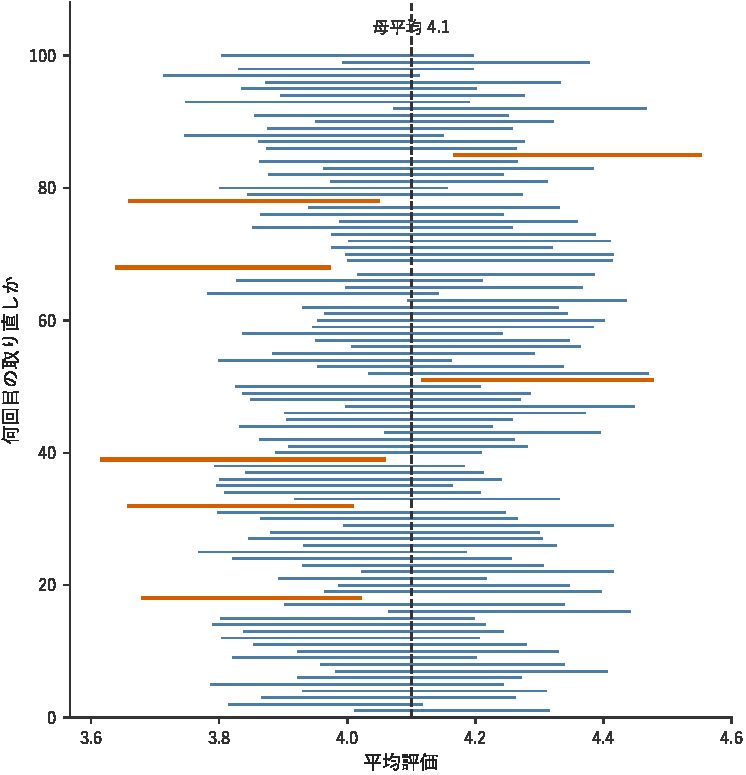
\includegraphics[width=0.8\linewidth]{../figures/output/ch05_ci_coverage.pdf}
      \caption{母平均4.1, 標準偏差0.7の仕組みから50件の標本を取り, 95\%信頼区間を作る手順を100回繰り返したシミュレーション. 横棒の1本1本が1回分の区間. 破線は母平均で, 動かない. 100本のうち93本(細い棒)は母平均を含み, 7本(太い棒)は外した.}
      \label{fig:ch05_ci_coverage}
    \end{figure}

    100本の区間は, どれも少しずつ違う場所にできている.
    そして, そのうち93本は $\mu = 4.1$ を含み, 7本は外した.
    95本ちょうどではないが, 100回の繰り返しをやり直せば, この本数は95前後で毎回すこし変わる.
    95\%とは, 一本一本の区間が持っている性質ではなく, この\textbf{手順の当たりやすさ}のことなのだ.

    では, 手元の一本, 4.0から4.4はどうか.
    図の中から棒を一本選んで「この区間は母平均を含んでいますか」と聞かれたら, 答えは含んでいるか, いないかの二つに一つだ.
    「95\%の確率で含んでいる」という状態は, 図のどこにもない.
    手元の区間も同じで, 当たりか外れかのどちらかであり, どちらなのかは $\mu$ を知らない私たちには分からない.

    それでも, この区間は信用して報告に使ってよい.
    ただし, 信用の根拠は区間そのものにではなく, 区間を作った手順の側にある.
    この手順で区間を作れば, 繰り返したとき95\%は母平均を含むように設計されている.
    手元の一本は, その手順から出てきた一本だ.
    だから95\%信頼区間は, 「この区間に $\mu$ がある確率が95\%」ではなく, 「\textbf{繰り返せば95\%当たる作り方で作った区間が, これだ}」と読む.
    区間を受け取った人も, 同じ読み方をすればよい.
    「100回中95回当たる手順の1回分」という意味合いさえ共有されていれば, 幅の解釈が人によって食い違うことはない.

    \subsubsection*{幅があると何が変わるか}

    読み方が定まったところで, 幅を添えることが実際の判断でどう効くかを見ておこう.

    新薬の治験で「血圧を平均5\,mmHg下げた」という結果が出たとする.
    95\%信頼区間が2〜8\,mmHgなら, 「少なくとも2\,mmHgは下がりそうだ」と見込める.
    医師はこの情報をもとに投薬を判断できる.
    ところが同じ「平均5下がった」でも, 区間が$-1$〜$11$\,mmHgなら話は変わる.
    幅の中にゼロやマイナスが入っている以上, 「効かない可能性も, むしろ上がる可能性も, 取り直しのばらつきの範囲内」ということになり, 判断は慎重にならざるをえない.
    点の値だけを見ていたら, この二つの状況は区別できない.

    幅を添えた報告は, 見積もりの値だけでなく, その見積もりの精度まで相手に渡す.
    過大な断言を防ぎ, 判断ミスを減らすのは, この「精度ごと渡す」働きだ.

    \subsubsection*{何\%にするかは, 人が決める}

    ここまでの手続きのうち, 何が理論から決まっていて, 何が人間の選択なのかを整理しておく.

    「$\bar{x}$ がおよそ正規分布に従う」という部分は, 中心極限定理から導かれる帰結だ.
    ここに人間の裁量は入っていない.
    一方, 「繰り返したとき何\%当たる手順にするか」は, 使う側が決めることだ.
    この割合を\textbf{信頼水準}と呼ぶ.
    信頼水準を決めると, 正規分布の形から, SEの何倍まで広げればよいかが対応して決まる.

    \begin{itemize}
      \item 90\%なら $\pm 1.64 \times \mathrm{SE}$
      \item 95\%なら $\pm 1.96 \times \mathrm{SE}$
      \item 99\%なら $\pm 2.58 \times \mathrm{SE}$
    \end{itemize}

    本書ではこの3行で足りる.

    99\%にすれば外す回数は100回中1回に減るが, そのぶん幅は広がる.
    90\%にすれば幅は狭くなるが, 10回に1回は外す手順になる.
    どのくらいの外れを許容するかは, 分析の目的に応じて選ぶものであり, 理論が一意に決めるものではない.
    95\%が広く使われているのは, 幅の狭さと外しにくさのバランスが実用上とりやすいからで, それ以上の根拠はない. 慣習だ.

  \subsection{やり方 : 3つのケースで幅を作る}

    \subsubsection*{前提}

    以降の計算が仮定するのは, 前章の中心極限定理と同じく, 観測値が独立同分布(i.i.d.)であることの1点である.
    標本サイズの大きさは前提ではなく近似の精度の問題であることも, 前章で整理したとおりだ.

    幅の作り方は, どのケースでも共通している.
    見積もりたい量の推定値を計算し, その推定値のSEを求め, 推定値 $\pm 2 \times \mathrm{SE}$ とする.
    ケースごとに変わるのは, SEの計算式だけだ.

    \subsubsection*{ケース1 : 平均に幅をつける}

    ある商品の重量を $n = 64$ 個測ったところ, 平均 $\bar{x} = 170$\,g, 標準偏差 $s = 12$\,gだった.

    SEは $12/\sqrt{64} = 12/8 = 1.5$\,g.
    95\%信頼区間は
    \[
      170 \pm 2 \times 1.5 \;\Rightarrow\; 167.0\;\text{g〜}\;173.0\;\text{g}.
    \]

    この幅が「広い」か「狭い」かは, 何と比べるかで決まる.
    たとえばこの商品の規格が「165〜175\,gに収まること」なら, 区間はすっぽり規格内に入っており, 安心材料になる.
    規格が「169〜171\,g」と厳しければ, 区間が規格からはみ出しており, $n$ を増やして見積もりの精度を上げるなどの対策が要る.
    幅そのものに良い悪いはなく, 評価は文脈が決める.

    \subsubsection*{ケース2 : 割合に幅をつける}

    20本の作品のうち, 平均評価が4.0以上のものが $k = 14$ 本だったとする.
    標本での割合は $p = 14/20 = 0.70$ だ.
    知りたいのは, 母集団全体でこの割合がいくらか, である.

    割合にも同じ作り方が通用する.
    各作品を「4.0以上なら1, 未満なら0」と数値にしてみると, 割合 $p$ はこの0と1の平均にほかならない.
    平均である以上, 中心極限定理がそのまま効いて, $p$ の取り直しのばらつきもおよそ正規分布に従う.
    そのSEは次の式で見積もれる.
    \[
      \mathrm{SE}(p) \approx \sqrt{\frac{p(1-p)}{n}} = \sqrt{\frac{0.70 \times 0.30}{20}} \approx 0.102.
    \]

    分子の $p(1-p)$ は, 0と1のデータの散らばりの大きさに当たる.
    $p$ が0.5に近いほど0と1が混ざり合って散らばりは大きく, 0や1に近いほど値が片側に揃って小さくなる.
    分母の $n$ は件数で, 多いほどSEは小さくなる.
    平均のSEと同じ構造だ.

    95\%信頼区間は
    \[
      0.70 \pm 2 \times 0.102 \;\Rightarrow\; 0.50\;\text{〜}\;0.90.
    \]

    かなり広い.
    「半分」から「9割」までの範囲では, 見積もりとしてほとんど絞り込めていない.
    $n = 20$ では, 割合の推定はこの程度の精度にとどまる.

    \subsubsection*{ケース3 : 2つの平均の差に幅をつける}

    グループAとBで, 値の平均を比べたいとする.
    見積もりたい量は平均の差 $\bar{x}_A - \bar{x}_B$ だ.
    2群が互いに独立である(AとBで別の個体から集めている)とき, 差のSEは各群の標準偏差 $s_A, s_B$ と件数 $n_A, n_B$ から見積もれる.
    \[
      \mathrm{SE}(\bar{x}_A - \bar{x}_B) \approx \sqrt{\frac{s_A^2}{n_A} + \frac{s_B^2}{n_B}}.
    \]

    根号の中は, それぞれの群の分散を件数で割ったものの和だ.
    $s_A^2/n_A$ は $\bar{x}_A$ の, $s_B^2/n_B$ は $\bar{x}_B$ のばらつき(SEの2乗)であり, 2群が独立なら, 差のばらつきはこの2つの足し算になる.
    引き算をしているのに, ばらつきのほうは差し引かれない.
    もし2群が連動して同じ方向にずれるなら, 差を取った時点でずれどうしが打ち消し合い, ばらつきは小さくなりうる.
    しかし独立なら, $\bar{x}_A$ のずれと $\bar{x}_B$ のずれは無関係に生じるから, 打ち消し合いは期待できず, どちらのずれもそのまま差に持ち込まれる.
    両方の変動が加わるぶん, ばらつきの大きさを表す分散は積み重なる.
    差がどちらか一方の平均だけよりも大きくばらつくのは, その結果だ.

    幅は同じく, 差 $\pm 2 \times \mathrm{SE}$ とする.
    差の区間を読むときは, まずゼロをまたぐかどうかを見る.
    またいでいれば, 「差がない(ゼロ)」も取り直しのばらつきの範囲内にあることになり, 差の向きすら言い切れない.
    またいでいなければ, 少なくとも差の向きは, ばらつきを見込んでも保たれている.

  \subsection{実践 : 80本の映画に幅を添える}

    ランニング例に戻ろう.
    手元にあるのは, 配信サービスの対象作品から抽出された邦画80本の標本だった.
    第1章で置いた「標本は対象作品全体から大きな偏りなく抽出されたものとして扱う」という仮定を, ここでも使う.
    3つのケースを順に当てはめて, 対象作品全体について幅つきで言えることを確かめていく.

    \subsubsection*{平均 : 視聴回数はどのくらいか}

    80本の視聴回数は, 平均 $\bar{x} = 209.4$ 万回, 標準偏差 $s = 239.3$ 万回だった.
    SEは
    \[
      \mathrm{SE} = \frac{239.3}{\sqrt{80}} \approx 26.8\;\text{万回}
    \]
    となり, 95\%信頼区間は
    \[
      209.4 \pm 2 \times 26.8 \;\Rightarrow\; 155.9\;\text{万回〜}\;262.9\;\text{万回}.
    \]

    報告するなら, たとえば次のような一文になる.
    「対象作品の平均視聴回数は209万回と推定される(95\%信頼区間 : 156万〜263万回).」
    信頼水準と幅を添えておけば, 受け手は「繰り返せば95\%当たる作り方での見積もり」として, 精度ごと受け取れる.

    \subsubsection*{割合 : 評価4.0以上の作品はどのくらいあるか}

    80本のうち, 平均評価が4.0以上の作品は33本だった.
    標本での割合は $p = 33/80 \approx 0.41$.
    SEは
    \[
      \mathrm{SE}(p) \approx \sqrt{\frac{0.41 \times 0.59}{80}} \approx 0.055
    \]
    となり, 95\%信頼区間は
    \[
      0.41 \pm 2 \times 0.055 \;\Rightarrow\; 0.30\;\text{〜}\;0.52.
    \]

    「対象作品のうち評価4.0以上は41\%と推定される(95\%信頼区間 : 30\%〜52\%)」となる.
    $n = 80$ あっても, 割合の幅は $\pm 11$ ポイントある.
    ケース2の $n = 20$ よりはずっと絞れているが, たとえば幅を $\pm 3$ ポイントまで詰めるには, 1000件ほどが必要になる.

    \subsubsection*{差 : 原作の有無で視聴回数は違うか}

    80本の映画には, 原作のある作品(既存作品の映画化)とない作品(オリジナル脚本)が混ざっている.
    原作あり37本の平均視聴回数は274.1万回(標準偏差257.1万回), 原作なし43本の平均は153.7万回(標準偏差207.2万回)で, 差は120.4万回だった.

    2群は別々の作品からなり, 独立とみなせる.
    差のSEは
    \[
      \mathrm{SE} \approx \sqrt{\frac{257.1^2}{37} + \frac{207.2^2}{43}} \approx 52.8\;\text{万回}
    \]
    となり, 95\%信頼区間は
    \[
      120.4 \pm 2 \times 52.8 \;\Rightarrow\; 14.8\;\text{万回〜}\;225.9\;\text{万回}.
    \]

    区間はゼロをまたいでいない.
    取り直しのばらつきを見込んでも, 「原作あり群のほうが多い」という向きは保たれている.
    ただし下端の14.8万回は, ゼロのすぐ近くだ.
    そして「15万回差」から「226万回差」までは, 差の大きさとしてほとんど別世界であり, 大きさのほうはまだ絞り込めていない.
    この結果をどこまで信じてよいかは, 章の終わりでもう一度考える.

  \subsection{幅を狭めたいとき}

    区間が広すぎて実用にならないと感じたら, 打てる手は3つある.

    第一に, $n$ \textbf{を増やす}.
    SEは $1/\sqrt{n}$ のペースで縮むから, $n$ を4倍にすれば幅は半分になる.
    「あと何件集めれば幅がどのくらい縮むか」を, この関係から前もって見積もれる.

    件数の効果を具体的に見ておこう.
    平均3.8, $s = 0.9$ のデータで, 件数だけが違う場合を比べる.
    \begin{itemize}
      \item $n = 5$ : $\mathrm{SE} = 0.9/\sqrt{5} \approx 0.40$ で, 幅は $\pm 0.80$
      \item $n = 20$ : $\mathrm{SE} = 0.9/\sqrt{20} \approx 0.20$ で, 幅は $\pm 0.40$
      \item $n = 100$ : $\mathrm{SE} = 0.9/\sqrt{100} = 0.09$ で, 幅は $\pm 0.18$
    \end{itemize}
    平均はどれも同じ3.8だ.
    しかし $n = 5$ の幅と $n = 100$ の幅は4倍以上違う.
    「平均が同じなら同じことを言っている」わけではない.
    レビューサイトで星4.2の店が2軒あっても, 件数5件の4.2と件数500件の4.2では, 見積もりとしての確かさがまるで違う.

    第二に, \textbf{ばらつき} $s$ \textbf{を下げる}.
    測定条件を安定させる, 対象を絞る, 性質の近い層に分けてから推定する, といった工夫で $s$ が小さくなれば, SEも縮む.

    第三に, \textbf{信頼水準を下げる}.
    95\%を90\%にすれば幅は狭くなる.
    ただし10回に1回外す手順になるので, 幅の狭さを外れやすさで買っていることになる.

    実務でまず検討するのは最初の2つだ.
    信頼水準の変更は見かけの幅を変えるだけで, 見積もりの精度そのものは何も変わっていない.

  \subsection{実務で気をつけること}

    \subsubsection*{偏りは$n$で解決しない}

    ここまでの話には, 見落とすと危険な前提が一つ埋まっている.
    「繰り返せば95\%当たる」という設計が成り立つのは, 手順の入り口, つまり標本の集め方がi.i.d.に近い場合だけだ.
    集め方が偏っていれば, $\bar{x}$ は取り直すたびに, 母平均からずれた場所を中心にばらつく.
    その状態で $n$ を増やすと, 区間は狭くなるのに, 区間の中心は的外れのままという結果になる.
    \textbf{精密に間違える}という, 最も危険な状態だ.
    区間の信用が手順の側にある以上, 手順が壊れていれば, どれほど狭い区間にも信用は残らない.
    区間の狭さに安心する前に, データの集め方をまず点検する.

    \begin{mybox}{ギャラップ vs.\ Literary Digest : 240万人が大はずれした話}
    1936年のアメリカ大統領選挙で, 雑誌 \textit{Literary Digest} は大規模な郵送調査を行った.
    返送されたのは約240万通.
    これだけの数があれば確実に思えるが, 予測は「ランドンの勝利」.
    結果はルーズベルトの圧勝で, 大はずれだった.

    原因は集め方にある.
    \textit{Literary Digest} は電話帳や自動車登録簿から名簿を作ったが, 1930年代にこれらを持っていたのは富裕層に偏っていた.
    さらに, 郵送に返事をする人としない人の間にも偏りがある.
    結果として, 240万人のデータは母集団を代表していなかった.

    一方, ジョージ・ギャラップはわずか約5万人の調査で正しくルーズベルトの勝利を予測した.
    ギャラップは年齢・性別・地域などの構成比を考慮して回答者を集める工夫をしていた.

    \textbf{$n = 240$万でも, 偏りがあれば自信満々に間違える}.
    この事件の後, \textit{Literary Digest} は廃刊に追い込まれた.
    \end{mybox}

    偏りの類型と対処は, 9章で改めて整理する.

    \subsubsection*{外れ値と歪みへの対処}

    平均とSDは外れ値に引っ張られやすい.
    3章でヒストグラムや箱ひげ図から外れ値に気づく方法を扱ったが, ここでの問題は, 外れ値が $\bar{x}$ と $s$ を通じて区間の位置と幅に直接響くことだ.
    きつい外れ値がある場合は, 中央値やIQRで要約し, 幅の作り方も\textbf{ブートストラップ}と呼ばれる別の方法に切り替えるほうが安全なことがある.
    ここでは名前だけの紹介にとどめる.

    データが右に強く歪んでいる場合は, 対数を取ってから扱うとよい.
    前章のコラムで見たとおり, 掛け算の仕組みから生まれた右裾の長い分布は, 対数を取ると足し算の世界に戻り, 釣鐘型に近づく.
    歪みが軽くなるぶん, 同じ $n$ でも正規近似の精度が上がる.
    対数のスケールで平均とSEを計算して幅を作り, 報告のときに必要なら元のスケールに戻す(戻した値は幾何平均に対応する).

    \subsubsection*{前処理の記録}

    推定の幅は, 期間の切り取り方, 欠損値の扱い, 外れ値の処理によって変わる.
    同じデータでも, 前処理が違えば違う区間ができる.
    「何を, いつ, どう集めて, どう処理したか」を明示しておくことが, 結果を他者と共有するための最低限の作法だ.

  \subsection{結果と次の一手 : 幅の先にある問い}

    前章の終わりに, SEを誰が読んでも同じ意味になる幅に直したい, という宿題を立てた.
    本章でその直し方が決まった.
    推定値 $\pm$ 約 $2 \times \mathrm{SE}$ で95\%信頼区間を作り, 平均・割合・差のどれにも同じ作り方を通せる.

    そして, 幅の読み方も決まった.
    95\%は区間そのものの性質ではなく, 区間を作る手順の当たりやすさだ.
    手元の一本が当たりか外れかは分からないが, 繰り返せば95\%当たる作り方で作った一本として報告し, 受け取る.
    この読み方さえ共有されていれば, 幅を添えた報告は, 見積もりの精度ごと相手に渡る.

    新聞の世論調査で「支持率45\%($\pm 3$ポイント)」という表記を見たことがあるかもしれない.
    あの $\pm 3$ ポイントは, まさにここで作った幅と同じものだ.
    次に見かけたら, 「繰り返せば95\%当たる手順の1回分」という意味合いまで読み取れるはずだ.

    最後に, 実践で残した宿題に戻る.
    原作あり群と原作なし群の平均視聴回数の差は, 95\%信頼区間で14.8万〜225.9万回だった.
    区間はゼロをまたがなかったが, 下端はゼロのすぐ近くにある.
    もし標本を取り直していたら, ゼロをまたぐ区間が出ていてもおかしくない.
    そうなると, 「原作あり群のほうが本当に多いのか, それとも, たまたま視聴回数の多い作品が原作あり側に集まっただけなのか」という疑いには, まだ決着がついていない.
    この「差は偶然のばらつきで説明できるか」という問いに正面から答えるには, 幅をつけるのとは別の枠組みが要る.
    それが, 次章で扱う\textbf{統計的検定}だ.

  \begin{mybox}{コラム : 標本平均は信用してよい見積もりか}
    本章では $\bar{x}$ のばらつきに幅をつけてきたが, そもそも $\bar{x}$ で $\mu$ を狙うこと自体は適切なのか, という一段手前の問いもある.
    母数の見積もりに使う統計量を\textbf{推定量}と呼び, その良し悪しを測る性質が知られている.

    一つは, 狙いが系統的にずれていないかだ.
    中心極限定理で見たとおり, $\bar{x}$ の標本分布の中心は母平均 $\mu$ そのものだった.
    取り直しを繰り返したときの $\bar{x}$ の平均が $\mu$ に一致する, つまり高めにも低めにも偏らない.
    この性質を\textbf{不偏性}といい, 標本平均は母平均の不偏推定量である.

    不偏でない例は, じつは第2章にすでに登場している.
    分散を $1/n$ で計算すると, 母集団の分散よりも系統的に小さめの値が出る.
    偏差を母平均 $\mu$ からではなく標本平均 $\bar{x}$ から測っているためだ.
    $\bar{x}$ は手元のデータに最も寄り添う位置に来る値なので, $\bar{x}$ からの偏差の2乗和は, $\mu$ からのそれより必ず小さめになる.
    その縮みぶんを補正したのが, $n$ の代わりに $n-1$ で割る\textbf{不偏分散}だ.
    第2章の脚注で触れた「$n-1$ で割る流儀」の正体は, この補正である.

    もう一つは, 件数を増やせば母数に近づいていくかだ.
    $\bar{x}$ のSEは $s/\sqrt{n}$ だから, $n$ を増やせば $\bar{x}$ の散らばりはいくらでも小さくなり, $\mu$ のまわりに絞り込まれていく.
    この性質を\textbf{一致性}と呼ぶ.

    狙いが系統的にずれず(不偏性), 数を増やせば絞り込める(一致性).
    統計学が標本平均を安心して使うのは, こうした性質の裏づけがあってのことだ.
    実務でここまで確かめる場面は少ないが, 推定量への信用がどこから来ているのかは, 知っておいて損はない.
  \end{mybox}


\newpage

\section{検定 -- 仮説と\texorpdfstring{$p$}{p}値をどう読むか}

  \subsection{この差は偶然か}

    前章の終わりに, 答えを保留した問いが一つ残っている.
    配信サービスの邦画作品の標本で, 原作のある作品（既存作品の映画化）と原作のない作品（オリジナル脚本）の平均視聴回数を比べたところ, 原作あり群のほうが多かった.
    ところが, 差に幅をつけてみると, 95\%信頼区間の下端はゼロのすぐ近くまで来ていた.
    標本を取り直していたら, ゼロをまたぐ区間が出ていてもおかしくない.
    この差を根拠に「原作の有無は視聴回数に効いている」と言ってよいのか.
    それとも, たまたま視聴回数の多い作品が原作あり側に偏っただけなのか.

    信頼区間からわかるのは, 差の見積もりがどのくらいの幅を持つかまでだ.
    目の前の差は, 偶然のばらつきとして片づけられる範囲に収まっているのか, それを超えているのか.
    この一歩踏み込んだ問いに白黒をつける手続きが, 前章の終わりに名前だけ挙がった\textbf{統計的検定}だ.

    同じ形の判断は, すでに身の回りのあちこちで使われている.
    選挙の開票速報で, 開票率がまだ数\%なのに「当選確実」が出る場面を見たことがあるだろう.
    あれは, 出口調査の標本に表れた候補者間の得票差が, 偶然では説明しにくいほど大きいかどうかを判断した結果だ.
    IT企業がWebサイトのボタンの色を変えてクリック率を比較する, いわゆるA/Bテストも同じ構造をしている.
    どの場面でも, 突き詰めれば二つのグループの数字を見比べる話である.
    見比べるだけなら, 平均を並べれば済みそうだ.
    まずはそこから試してみる.


  \subsection{目で見た差は当てになるか}

    二つのグループの平均を計算して, 差を見る.
    差が大きければ「違いがある」, 小さければ「違いはない」.
    日常の多くの場面で, 実際にこうやって判断している.

    たとえば, 二つのクラスの英語テストの平均点を比べるとしよう.
    A組の平均は72点, B組の平均は68点で, 4点の差がある.
    「けっこう違う. 教え方に差があったのではないか」と感じる人もいるだろう.

    ここで, 前章の計算を持ち込んでみる.
    各クラスの人数が15人で, 標準偏差が12点だったとする.
    前章のケース3で使った「差の標準誤差」を計算して, 二つのグループの平均の差が偶然でどのくらいばらつきうるかを見積もる.
    %
    \[
      \mathrm{SE}_{\text{差}} = \sqrt{\frac{12^2}{15} + \frac{12^2}{15}} = \sqrt{9.6 + 9.6} \approx 4.4 \text{ 点}
    \]
    %
    根号の中の各項は, 各グループの分散を人数で割った$s^2 / n$で, それぞれ$12^2 / 15 = 9.6$だ.
    前章で見たとおり, 二つのグループが独立なら, 差のばらつき（分散）はそれぞれのばらつきの足し算になる.
    結果はおよそ4.4点.
    観測された差の4点より, 偶然で見込まれるばらつきのほうが大きい.
    二つのクラスの母平均がまったく同じだったとしても, 標本平均の差は4点程度まで容易にばらつく, ということだ.

    平均点だけ見れば「けっこう違う」ように映る72点と68点も, 一人ひとりの点数が12点もばらつく中では, 偶然の差と区別がつかない.
    \textbf{差の大きさだけでは, 意味のある差かどうかは判断できない.}
    ばらつきと人数を織り込んだ, 判断の組み立てが要る.


  \subsection{「差がない世界」を出発点にする}

    二つのグループに差があるかどうかを調べたい.
    素朴に考えれば, 「差がある」ことを直接示しにいけばよさそうだ.
    ところが, ひとくちに「差がある」と言っても, その中身は一つに決まらない.
    2点の差も「差がある」だし, 10点でも0.001点でも「差がある」.
    「差がある世界」は無数にあって, 議論の出発点をどこに置けばよいのかが定まらないのだ.

    一方, 「差がゼロ」の世界はただ一つに決まる.
    そこで検定では, 発想を逆転させる.
    \textbf{「差がない世界」を仮に設定する}ことから始めるのだ.
    この世界では, 二つのグループの母平均は等しく, 観察される差はすべて偶然のばらつきから生じる.
    その世界を基準にして, 手元のデータに出た差がどのくらい珍しいかを確率で測る.
    もし「差がない世界ではめったに起こらない」ほど珍しければ, 差がないという仮定のほうに無理があると判断する.

    この「差がない」側の仮定を\textbf{帰無仮説}（$H_0$）と呼ぶ.
    対して, 「差がある」という主張を\textbf{対立仮説}（$H_1$）と呼ぶ.
    帰無仮説という名前は物々しいが, 中身は「差がない側の仮定」以上のものではない.
    ただ, 論文や記事には頻繁に出てくる用語なので, 名前を知っておくと読むときに困らない.

    \subsubsection*{差を標準化する}

    手元のデータに出た差の珍しさを, 差がない世界を基準にして測りたい.
    ところが, 前の節で見たとおり, 4点という差が大きいのか小さいのかは, データのばらつきと人数によってまったく変わる.
    差をそのまま眺めても, 珍しさの見当がつかない.

    そこで, 差をそのばらつき（標準誤差）で割って標準化する.
    前章の信頼区間でも, $\bar{x}$と$\mu$のずれを$\mathrm{SE}$の何倍分と数えて幅を作っていた.
    検定でも同じ発想を使う.
    この標準化した値を\textbf{検定統計量}と呼ぶ.
    たとえば二つの平均の差を比べるなら,
    %
    \[
      t = \frac{\text{二つの平均の差}}{\text{差の標準誤差}}
    \]
    %
    分子は差の大きさで, 分母はその差が偶然でどのくらいばらつくかである.
    差が大きいほど, ばらつきが小さいほど, 人数が多いほど, この値は大きくなる.
    ばらつきで測り直した値は, テストの点数やクリック率といった元の単位を引きずらない.
    だから, 種類の違うデータでも, 差の珍しさを同じ基準で比べられる.

    問いの種類に応じて, 使う検定統計量は変わる.
    平均の差なら$t$統計量, カテゴリの偏りならカイ二乗統計量$\chi^2$, ばらつきの比なら$F$統計量だ.
    統計量が違っても, 「差を標準化して珍しさを測る」という構造は同じである.
    どれを使うかは問いの形で決まるので, すべてを暗記する必要はない.

    \subsubsection*{珍しさを数値にする：\texorpdfstring{$p$}{p}値}

    検定統計量が, たとえば$t = 2.3$と出たとしよう.
    この数字だけを眺めていても, 「珍しい」のか「よくある」のかは判断がつかない.

    頼りになるのは, 帰無仮説のもとで検定統計量がどんな値をとりやすいか, という分布である.
    差がない世界でも, 偶然のばらつきのせいで$t$はゼロちょうどにはならず, ゼロの周りに散らばる.
    その散らばり方は理論的にわかっていて, 平均の差の$t$統計量なら\textbf{$t$分布}, カテゴリの偏りのカイ二乗統計量ならカイ二乗分布と呼ばれる分布に従う.
    この分布の中で, いまの値と同じかそれ以上に極端な値が出る確率を求める.
    それが\textbf{$p$値}である.
    $p$値が小さいほど, 差がない世界では起こりにくい結果が出ている, と読める.

    ここで, 「$p$値が小さいなら, 帰無仮説が正しい確率が低いのだろう」と読みたくなるかもしれない.
    しかしそうではない.
    $p$値は, 帰無仮説が正しい\textbf{と仮定したうえで}計算した確率であって, 帰無仮説そのものが正しいかどうかの確率ではない.

    がん検診に同じ構造がある.
    検診で「陽性」と出ても, 実際にがんである確率は数\%にとどまることがある.
    「陽性」が意味しているのは「がんがないとしたら, この検査結果は珍しい」というところまでで, 「がんである確率が高い」こととは別の話だ.
    $p$値と帰無仮説の関係も, 同じ形をしている.

    \subsubsection*{判断の基準を先に決める}

    $p$値の「どのくらい小さければ珍しいと言えるか」を, その都度決めていたらどうなるか.
    都合のよい結果が出たときだけ, 「$p = 0.06$だけど, まあ有意と言ってもいいだろう」と基準を緩めたくなる.

    この恣意性を防ぐために, 判断の基準となる値を\textbf{有意水準}（$\alpha$）と呼び, 検定の前に決めておく.
    広く使われているのは$\alpha = 0.05$で, 差がない世界でも20回に1回は有意という結果が出てしまう程度の線にあたる.
    0.05という数字に絶対的な根拠があるわけではない.
    歴史的な慣習として定着したものだ.

    ただし, どの分野でも0.05というわけではない.
    素粒子物理学では「5$\sigma$」と呼ばれる基準が使われており, $p \approx 0.0000003$に相当する.
    ヒッグス粒子の発見で採用された基準だ.
    人命に関わる医薬品の認可でも, 通常より厳しい基準が求められることがある.
    どこに線を引くかは, 判断を間違えたときのコストに応じて人間が決めることなのだ.

    \begin{mybox}{新薬の認可と二つの誤り}
      新薬の治験では, 二つの誤りが問題になる.
      一つは, 効かない薬を「効く」と判断してしまう誤り（\textbf{第I種の誤り}）.
      もう一つは, 効く薬を「効かない」と判断してしまう誤り（\textbf{第II種の誤り}）.
      第I種の誤りが起こる確率は, 有意水準$\alpha$で抑えられる.
      第II種の誤りは, サンプルサイズを大きくすることで減らせる.
      アメリカのFDA（食品医薬品局）の新薬認可では通常$p < 0.05$が要求されるが,
      がん治療薬のように「効く薬を承認しないこと」のコストが大きい場面では, 基準が変わることもある.
      0.05という数字そのものは慣習でも, どの水準を採るかは誤りのコストとの相談で決まっている.
    \end{mybox}

    「$p = 0.04$なら有意で, $p = 0.06$なら有意でない. 境界の前後でそんなに違うものか」と感じるかもしれない.
    もっともな疑問で, 実際, 0.04と0.06のあいだで何かが不連続に変わるわけではない.
    $p$値は連続的な指標であり, 有意水準は便宜上の区切り線にすぎない.
    $p$値だけで白黒をつけることの限界は多くの統計学者が指摘しており,
    効果の大きさやサンプルサイズとあわせて判断することが求められている.


  \subsection{検定の手順}

    ここまでの部品を並べ直すと, 検定は「差がない世界を仮に設定し, 手元のデータがその世界でどのくらい珍しいかを調べる」手続きとしてまとまる.

    ただし, どんなデータにでも使えるわけではない.
    観測どうしが独立であること（ある観測が別の観測に影響していないこと）, 比較するグループの定義が明確であること, そして有意水準を検定の前に決めてあることが前提になる.
    このうえで, 次の5つのステップを順に踏む.

    \begin{enumerate}
      \item \textbf{何を比較するかを決める.}
        調べたい問いに応じて, 適切な統計量を選ぶ.
        二つのグループの平均を比べたいなら$t$統計量,
        カテゴリの偏りを調べたいならカイ二乗統計量$\chi^2$,
        ばらつきの比を見たいなら$F$統計量だ.
        統計量の選択を間違えると, 「答えが出てこない」のではなく「的外れな問いに答えてしまう」ことになる.

      \item \textbf{帰無仮説を立てる.}
        「差がない」「効果がない」「関係がない」と仮定する.
        帰無仮説のもとで検定統計量が従う分布は理論的にわかっているので, 珍しさを確率として計算できる.

      \item \textbf{データから検定統計量を計算する.}
        実際のデータを使って, 差をばらつきで標準化した値を求める.

      \item \textbf{帰無仮説のもとでの分布から$p$値を求める.}
        帰無仮説が正しいとしたとき, 計算した統計量と同じかそれ以上に極端な値が出る確率だ.

      \item \textbf{$p$値と有意水準を比較して判断する.}
        $p$値が有意水準$\alpha$より小さければ, 帰無仮説のもとでは今のデータは珍しすぎると判断し,
        帰無仮説を\textbf{棄却}する. 対立仮説, つまり「差がある」という主張が支持される.
        $p$値が$\alpha$以上であれば, 帰無仮説を棄却できない.
    \end{enumerate}

    「帰無仮説を棄却できない」ことと「差がない」ことは同じではない.
    裁判にたとえるなら, 「証拠不十分で無罪」と「無実の証明」は異なる.
    今回のデータでは帰無仮説を退けるだけの証拠が見つからなかった, というだけだ.
    差が本当にゼロであると積極的に主張しているわけではない.
    「差がないこと」を直接示すには, 同等性検定という別の手順が必要になる.
    本書では扱わないが, 必要になったときに調べればよい.

    \subsubsection*{片側検定と両側検定}

    検定の前に決めておくのは, 有意水準だけではない.
    問いの向きも, データを見る前に決めておく必要がある.
    「原作あり群のほうが高い」と問うのか, 向きを決めずに「単に差がある」と問うのかで, $p$値の計算方法が変わるからだ.

    特定の方向にだけ関心がある場合を\textbf{片側検定}, 方向を問わない場合を\textbf{両側検定}と呼ぶ.
    片側検定では「極端」の定義が分布の片方の裾だけになるため, $p$値は両側の場合の半分になる.
    同じデータでも, 問い方が変われば結論が変わりうる.
    検定は, データから問いを探し出す手続きではなく, あらかじめ立てた問いに答える手続きなのだ.

    迷ったときは両側検定を選ぶのが安全だ.
    片側検定を使うのは, 理論的に一方向しかありえない場合や, データを見る前に方向まで決めていた場合に限る.
    分析が終わってから都合のよい方向を選ぶのは, 判断の基準を後から緩めるのと同じことになる.

    \begin{mybox}{\textit{Student}とビール工場}
      $t$統計量を考案したのは, ウィリアム・ゴセット（1876--1937）というイギリスの統計学者だ.
      彼はダブリンのギネス醸造所で品質管理を担当していた.
      少数のビールサンプルから品質を判断しなければならないという実務的な動機から,
      小標本でも使える検定法を開発した（1908年）.
      会社の規定で本名での論文発表ができなかったため, ``Student''というペンネームを使った.
      $t$分布を``Student's $t$''と呼ぶのはこのためだ.
    \end{mybox}


  \subsection{原作の有無で平均視聴回数に差はあるか}

    冒頭の問いに, 検定の手順を当てはめてみよう.

    手元の標本にある作品を, 原作の有無で二つのグループに分ける.
    一方は原作のある作品の集まり（原作あり群）,
    他方は原作のない作品の集まり（原作なし群）だ.
    このように, 別々の対象を二つのグループに分けて比べる方法を\textbf{対応のない二群の比較}と呼ぶ.

    5つのステップに沿って進める.

    何を比較するかは決まっている.
    二つのグループの平均視聴回数だから, $t$統計量を使う.
    帰無仮説は「原作の有無によって平均視聴回数に差はない」.
    対立仮説は「原作あり群のほうが平均視聴回数が高い」とする.
    方向を指定しているので, 片側検定にあたる.
    「単に差があるかどうか」だけを知りたいなら両側検定になる.
    どちらにするかは, データを見る前に決めておくのだった.

    検定統計量は, 二つのグループの平均とばらつきから$t$統計量として計算する.
    $p$値は, 「平均視聴回数に差がない」と仮定したときに, 得られた$t$統計量と同じかそれ以上に極端な値が出る確率として, $t$分布から求める.
    具体的な計算はPart Bで手を動かしながら確認する.

    あらかじめ有意水準を$\alpha = 0.05$と決めていたとしよう.
    $p$値が0.05より小さければ帰無仮説を棄却し, 「原作あり群のほうが平均視聴回数が高い」という主張が支持される.
    0.05以上であれば, 帰無仮説は棄却できない.

    ただし, 仮に有意な差が出たとしても, 「原作の有無」そのものが視聴回数を押し上げたとまでは言い切れない.
    原作のある作品は知名度や製作費, 宣伝規模が大きい傾向があり, その違いが視聴回数の差として表に出ている可能性がある.
    検定で言えるのは「平均視聴回数の差は偶然では説明しにくい」というところまでで, 何がその差を生んだのかには別の議論が要る.
    この種の入り組んだ関係は, 9章で改めて扱う.

    章の冒頭で, 差の95\%信頼区間の下端がゼロのすぐ近くまで来ていることを気にしていた.
    あのとき見ていたものは, 実は検定と同じである.
    二つの平均の差の95\%信頼区間がゼロを含んでいなければ, 有意水準5\%の両側検定で帰無仮説は棄却される.
    逆にゼロを含んでいれば, 棄却できない.
    信頼区間は差の大きさを幅で見積もり, 検定は「偶然で説明できるか」に判定を下す.
    同じ情報を, 別の角度から読んでいるのだ.
    この対応も, Part Bの計算で確かめられる.


  \subsection{血液型と性格をカイ二乗検定で調べる}

    今度は, 量的データではなくカテゴリデータの検定を見てみよう.

    一昔前に, 血液型によって性格がわかるという診断が流行したことがある.
    「A型は几帳面, B型はマイペース」といった話だ.
    こうした主張に科学的根拠があるかどうかはひとまず脇に置いて,
    「血液型と性格に関係があるのか」をデータで調べるとどうなるかを見ていく.

    100人に「血液型」と「性格タイプ（几帳面／大雑把）」を聞いた結果が, 次のクロス集計表にまとまっているとする.

    \begin{center}
      \begin{tabular}{l|cccc|c}
             & A型 & B型 & O型 & AB型 & 合計 \\
      \hline
      几帳面 & 18  & 6   & 10  & 8    & 42 \\
      大雑把 & 7   & 19  & 15  & 17   & 58 \\
      \hline
      合計   & 25  & 25  & 25  & 25   & 100
      \end{tabular}
    \end{center}

    A型で「几帳面」と答えた人は18人.
    他の血液型より明らかに多く, 「A型は几帳面」という俗説を裏づけているように見える.

    その「多い」は, 何と比べての多さだろうか.
    全体では100人中42人が「几帳面」と答えており, 各血液型は25人ずつだ.
    もし血液型と性格がまったく無関係なら, どの血液型でも几帳面な人は$25 \times 42/100 = 10.5$人くらいになるはずである.
    この10.5人を\textbf{期待度数}と呼ぶ.
    「無関係だとしたら, 行の合計と列の合計の比率から, 表の各マスにはこのくらいの人数が入るはず」という数値だ.

    A型で几帳面な人は18人で, 無関係なら10.5人程度.
    たしかにずれている.
    問題は, このずれが偶然でも起こりうるのか, それとも偶然では説明しにくいのか, である.

    手順は先ほどの$t$検定と同じ構造をたどる.
    帰無仮説は「血液型と性格タイプは無関係である」.
    各マスについて, 行合計$\times$列合計$\div$全体で期待度数を計算する.
    次に, 実際の人数と期待度数のずれを, すべてのマスについて集計してカイ二乗統計量を求める.
    ずれが大きいほど, カイ二乗統計量は大きくなる.
    最後に, 帰無仮説のもとでのカイ二乗分布から$p$値を求め, 有意水準を下回れば「無関係とは考えにくい」と判断する.
    具体的な計算はPart Bで確認する.

    カイ二乗検定の発想には100年以上の歴史がある.
    カール・ピアソンが1900年に, サイコロの出目が本当に均等かどうかを調べるために考案したのが始まりだ.

    なお, 仮にこの検定で有意な結果が出たとしても, それだけで「血液型と性格に関係がある」とは言い切れない.
    「血液型の俗説に合わせて回答してしまう人がいる」「性格の分類が恣意的である」など, データの集め方に由来する偏りが結果に影響している可能性があるからだ.
    検定にできるのは, データ上の偏りが偶然では説明しにくいと示すところまでで, その偏りが何に由来するかは検定の外の問題である.
    調査設計やバイアスの問題は9章で改めて扱う.


  \subsection{何がわかって, 何がまだ足りないか}

    出発点は, 「二つのグループに見えた差は, 偶然のばらつきで説明できるのか」という問いだった.
    目で見た差をそのまま信じると, 判断を誤ることがある.
    そこで, 差がない世界を仮に設定し, ばらつきとサンプルサイズを織り込んだうえで, 手元のデータの珍しさを測る.
    この枠組みが統計的検定だった.

    枠組みを支える部品は四つある.
    帰無仮説と対立仮説で問いを定式化し, 検定統計量で差を標準化し, $p$値で珍しさを数値に直し, 有意水準で判断の基準を事前に固定する.
    この四つがそろって初めて, 「この差は偶然で説明できる範囲か」を, 誰がやっても同じ手順で判断できる.

    ただし, 検定が答えているのは「偶然で説明できるか」までで, 「意味のある差か」には答えていない.
    ある健康食品の臨床試験を想像してほしい.
    10万人規模の調査で, 食品を摂取したグループの血圧が平均0.3\,mmHg低かったとする.
    $\mathrm{SE}$は$\sigma / \sqrt{n}$で計算するから, $n = 100{,}000$ともなると$\mathrm{SE}$は非常に小さくなり, 0.3\,mmHgの差でも$p < 0.001$となりうる.
    しかし, 0.3\,mmHgは血圧計の測定誤差の範囲にすら収まるような差で, 臨床的にはまったく意味がない.
    \textbf{「統計的に有意」であることと「実用的に意味がある」ことはまったく別}である.
    サンプルサイズが巨大なら, どんなに小さな差でも$p$値は小さくなる.
    逆にサンプルサイズが小さければ, 本当に差があっても検出できないことがある.
    $p$値が小さいことは, 「帰無仮説が間違っている」ことの証明でも, 「効果が大きい」ことの証拠でもない.
    差の大きさそのものは, 効果量という別の指標で測る.
    Part Bと9章で改めて扱う.

    2011年には, 心理学者ダリル・ベムが「未来予知」の実験で$p < 0.05$を得て一流誌に論文が掲載され, のちの追試では再現されない, という事件も起きている.
    $p$値だけで結論を出すことの危うさを象徴する事例だ.

    本章では, 検定が何をする手続きなのか, なぜそうするのかを, 数式を最小限にして追ってきた.
    次のPart Bでは, 同じ道を計算で歩き直す.
    二群の$t$検定（Welch法）とカイ二乗検定を実際に手で計算しながら,
    検定統計量がどう求まり, 自由度がどう決まり, $p$値がどう読めるのかを確かめていく.


\newpage

\section{統計的検定と推定 : 数学的背景と応用}
  \subsection{一致性と不偏性}

    Part Aでは, 標本から検定統計量を計算し, 帰無仮説のもとでの珍しさを測って判断を下す, という検定の流れを追った.
    Part Bでは, その中身を数式と数値で確かめていく.

    検定で本当に比べたいのは, 手元の標本そのものではなく, その背後にある母集団どうしである.
    たとえばサプリの効果を知りたいなら, サプリを飲んだ人の全体と飲んでいない人の全体を比べられれば, 話はそこで終わる.
    しかし, そんな大きな集団のデータを丸ごと手に入れるのは現実的ではない.
    そこで, 母集団の情報（母数）を標本からもっともらしく推定し, その推定値どうしを比べることになる.

    すると今度は, 推定のもっともらしさをどう評価するかが問題になる.
    その観点として, 5章の終わりのコラムでも触れた二つの性質がある.

    \begin{itemize}
      \item \textbf{一致性：} サンプルサイズを大きくしていくと, 推定量が母数に限りなく近づいていく.
      \item \textbf{不偏性：} 推定量の期待値が母数と一致する.
    \end{itemize}

    ぱっと見にはよく似ていて, 同じことを言っているようにも見える.
    しかし, 別の性質である\footnote{たとえば, サンプルサイズが大きくなってもノイズの影響が消えないような推定量では, 不偏性はあるのに一致性はない, ということも起こり得る.}.
    一致性はとても自然な要求だが, 一致性だけでは, 莫大な数のデータを集めないと母数に十分近づかない場合もある.
    そこを補うのが不偏性である.
    推定量の期待値が母数と一致するなら, 推定の狙いは平均的には高くも低くも偏っていない.
    サンプルサイズが限られた手元のデータからの推定でも, 系統的なずれを心配せずに扱える.
    このように一致性と不偏性は互いに補い合う性質で, 検定に使う推定量には両方を備えたものを選ぶのが基本になる.
    標本平均はその代表例で, 一致性と不偏性の両方を持っている.


  \subsection{自由度}

    本章の検定には, この後\textbf{自由度}という量が繰り返し登場する.
    t分布の形は自由度で決まり, カイ二乗分布の形も自由度で決まる.
    つまり, 自由度を取り違えると, 同じ検定統計量からでも違う$p$値が出てしまう.
    $p$値に直結する量でありながら, 自由度は「データの数から1を引いたもの」という公式の形で丸暗記されがちで, 意味を問われると答えに困る量でもある.

    幸い, 自由度の意味が最もはっきり見える場面が一つある.
    母集団の分散を標本から推定する場面だ.
    そこから話を始めよう.

    \subsubsection*{母集団の分散を推定したい. ところが母平均がわからない}

    母集団の分散（母分散） $\sigma^2$ は, 母集団の各データが母平均 $\mu$ からどれだけずれているかの二乗を, 母集団全体で平均した量である.
    各データのずれを二乗して足し, データ数で割る.
    式で書けば $\sigma^2 = \dfrac{1}{N}\sum (X_i - \mu)^2$ のようになるが, 構造としては「平均からのずれの二乗の平均」と覚えておけば十分だ.

    では, 手元の標本からこの量を推定したい.
    ここで困った事態に直面する.
    定義の中身に登場する $\mu$ がわからない.
    そもそも母集団のことが直接わからないからこそ, 標本を使って推定しようとしているのだった.
    それなのに, 推定したい量の定義の中に, もう一つの「わからない」量が入っている.

    打開策はひとつしかない.
    手元の標本から計算できる量で $\mu$ を代用する.
    最も自然な代用品は, 標本平均 $\bar{X} = \frac{1}{n}\sum X_i$ だ.
    そこで $\mu$ を $\bar{X}$ で置き換えた量
    \[
      \frac{1}{n} \sum_{i=1}^n (X_i - \bar{X})^2
    \]
    を考えてみたくなる.
    第2章で定義した分散と同じ形だし, これでうまくいきそうな気もする.
    しかし, この素直な置き換えには, ひとつ落とし穴がある.

    \subsubsection*{\texorpdfstring{$\bar{X}$}{X̄} で置き換えると, 何がずれるのか}

    $\bar{X}$ で代用したとき, 本当に知りたい量とどれくらい差が出るのかを調べてみよう.
    母分散の分子に当たる $\sum(X_i - \mu)^2$ と, 標本から計算する $\sum(X_i - \bar{X})^2$ の差を計算する.

    手始めに, $X_i - \mu = (X_i - \bar{X}) + (\bar{X} - \mu)$ と分解してから二乗を展開する：
    \begin{align*}
      \sum_{i=1}^n (X_i - \mu)^2
      &= \sum_{i=1}^n \left[ (X_i - \bar{X}) + (\bar{X} - \mu) \right]^2 \\
      &= \sum_{i=1}^n (X_i - \bar{X})^2 + 2(\bar{X} - \mu) \sum_{i=1}^n (X_i - \bar{X}) + \sum_{i=1}^n (\bar{X} - \mu)^2
    \end{align*}
    第二項の和の部分 $\sum (X_i - \bar{X})$ は, $\bar{X}$ の定義から常にゼロになる.
    よって第二項そのものが消える.
    結果として
    \[
      \sum_{i=1}^n (X_i - \mu)^2 = \sum_{i=1}^n (X_i - \bar{X})^2 + n(\bar{X} - \mu)^2
    \]
    が得られる.

    左辺は, 各データが\textbf{母平均から}どれだけずれているかの総量で, 本当に知りたい量である.
    第一項は, 各データが\textbf{標本平均から}どれだけずれているかの総量で, こちらは手元で計算できる.
    残る第二項は, 代用品の $\bar{X}$ 自身が本物の $\mu$ からどれだけずれているかを, データ全体分（$n$倍）まとめた量だ.

    つまり, 本物の $\mu$ から測ったずれの総量と, 代用品の $\bar{X}$ から測ったずれの総量は, 「$\bar{X}$ 自身のずれ」の分だけ食い違う.
    分解の式で, その食い違いが第二項として取り出せた.
    では, この食い違いは, どのくらいの大きさなのか.
    期待値を取って測ってみよう.

    \subsubsection*{ずれの大きさはデータ何個分にあたるか}

    上の式の各項の期待値を求めて, 大きさを比べる.

    左辺の期待値は, 母分散の定義から各 $X_i$ について $E[(X_i - \mu)^2] = \sigma^2$ なので
    \[
      E\!\left[\sum_{i=1}^n (X_i - \mu)^2\right] = n\sigma^2
    \]
    である.
    各データが「母平均から $\sigma^2$ 分ずれる」のを $n$個足したぶん, ということだ.

    第二項はどうか.
    4章で見たように, 標本平均 $\bar{X}$ 自体が母平均からどれだけずれるかは標準誤差で測れて, その分散は $\sigma^2/n$ だった.
    つまり $E[(\bar{X} - \mu)^2] = \sigma^2/n$.
    したがって
    \[
      E[n(\bar{X} - \mu)^2] = n \cdot \frac{\sigma^2}{n} = \sigma^2
    \]
    となる.

    第二項の期待値は $\sigma^2$ ちょうど, データひとつ分の分散ぴったりである.
    偶然ではなく, 構造的な必然だ.

    どういうことか.
    標本平均 $\bar{X}$ は, 母平均 $\mu$ を推定するために, $n$個のデータの中心の情報を一つの数に集約した量だ.
    そこまでは順当である.
    問題は, この $\bar{X}$ を, さらに分散の推定にも使い回そうとした点にある.
    本当に欲しいのは, 各データが母平均 $\mu$ からどれだけずれているかの総量（左辺）だった.
    しかし手元で計算できるのは, 各データが標本平均 $\bar{X}$ からどれだけずれているかの総量（第一項）である.
    平均の推定と分散の推定を, どちらも同じ $n$個のデータで済まそうとしたために, 中心を $\bar{X}$ で代用した代償が生じる.
    その代償の大きさが, 期待値で測るとちょうどデータひとつ分の分散 $\sigma^2$ なのだ.

    \subsubsection*{自由度 \texorpdfstring{$n-1$}{n-1} の意味}

    左辺の期待値が $n\sigma^2$, 第二項の期待値が $\sigma^2$ なので, 第一項の期待値は引き算で
    \[
      E\!\left[\sum_{i=1}^n (X_i - \bar{X})^2\right] = n\sigma^2 - \sigma^2 = (n-1)\sigma^2
    \]
    と求まる.

    手元で計算できる $\sum(X_i - \bar{X})^2$ が持っているずれの情報は, 期待値でみると, 本当に欲しかった $n\sigma^2$ よりデータひとつ分だけ少ない.
    だから, この量を $n$ で割ると, 母分散より少し小さめの値が出やすい.
    一方, $n-1$ で割れば, 期待値はちょうど $\sigma^2$ に一致する.
    平均的には母分散をぴったり言い当てる量になるわけだ.

    この $n-1$ で割った量を\textbf{不偏分散}と呼ぶ：
    \[
      s^2 = \frac{1}{n-1} \sum_{i=1}^n (X_i - \bar{X})^2
    \]
    \textbf{不偏}とは, 期待値を取ったときに偏りなく母数に一致する性質のことで, 前節の不偏性がこれにあたる.
    また, 大数の法則から, $n$ を大きくすれば標本平均 $\bar{X}$ は母平均 $\mu$ に近づくので, 不偏分散も $n$ を大きくすれば母分散に近づく.
    つまり一致性も併せ持つ
    \footnote{
      第2章で定義した分散は $n$ で割るものだった.
      あちらは手元のデータの散らばりをそのまま要約する量, こちらは母分散を狙う推定量で, 役割が違う.
      $n$ で割る版は不偏ではないが, 一致性は持つ.
      第2章の脚注で予告した「$n-1$ で割る理由」の答えが, この節の計算である.
    }.

    手元の $n$個のデータから出発して, $\bar{X}$ という一つの代表値に集約する過程で, 使える情報がデータひとつ分だけ目減りした.
    残った情報の個数が, データの数 $n$ から一つ引いた $n-1$ である.
    この数を\textbf{自由度}と呼ぶ.
    分散を $n-1$ で割って不偏にする補正は, 目減り分の埋め合わせだ.
    集約の代償として失われた一個分を, 分母を一つ減らすことで取り戻している.

    極端な場合で確かめておこう.
    データが1個しかないとき, 標本平均はそのデータ自身になり, ずれの総量 $\sum(X_i - \bar{X})^2$ は必ずゼロになる.
    ゼロを $n = 1$ で割れば「分散はゼロ」, つまり「母集団はまったくばらついていない」という見積もりが出てくるが, データ1個でばらつきの話ができるはずがない.
    一方, $n - 1 = 0$ で割ろうとすると, 値は定まらない.
    ばらつきの情報が何も残っていないから見積もり不能, という答えであり, こちらのほうが実態に合っている.
    平均の推定に1個分の情報を使い切ると, ばらつきに回せる情報はゼロになる.
    自由度ゼロとは, そういう状態のことだ.

    \subsubsection*{もう一つの見方: 標本平均を固定して残りの自由さを見る}

    自由度 $n-1$ を, もう一つ別の角度から眺めてみたい.
    この後のt検定やカイ二乗検定に出てくる自由度も, 同じ角度から数えられる.

    標本から $\bar{X}$ を計算した.
    ここで, $\bar{X}$ の値を一旦固定する.
    そのうえで, 「同じ標本平均をもつ別のデータの組」を考えてみる.
    つまり, $\frac{1}{n}\sum X_i = \bar{X}$ という条件を満たしたまま, $X_1, \ldots, X_n$ を動かしてみるということだ.

    この条件のもとでは, $X_1, \ldots, X_{n-1}$ までは自由に動かせる.
    しかし最後の $X_n$ は
    \[
      X_n = n\bar{X} - \sum_{i=1}^{n-1} X_i
    \]
    と自動的に決まってしまう.
    平均を $\bar{X}$ に合わせるためには, 最後の一つで帳尻を合わせるしかないからだ.
    自由に動かせる個数は $n-1$ にとどまる.

    この $n-1$ という数は, 元のデータそのものに最初から制約があるという話ではない.
    元のデータは $n$個とも自由に観測される.
    しかし, そこから $\bar{X}$ という代表値を計算して固定したうえで, 残ったずれ $(X_i - \bar{X})$ を眺めると, ずれの組が自由に動ける余地は $n-1$個分しかない.
    平均を引いたあとのずれに残された, 自由さの個数.
    「自由度」という名前は, この見方から来ている.

    この見方と, 前段の「集約の代償」は, 同じ事情の別の表れである.
    $\bar{X}$ という代表値を作って固定したことが, 期待値の計算では「データひとつ分の分散が代償として現れる」形で見え, ずれの動きに注目すると「自由に動ける個数が一つ少ない」形で見える.

    \subsubsection*{自由度は分散の推定だけの話ではない}

    ここまでは分散の推定を舞台にしてきたが, 同じ構造は統計的検定のあちこちにある.
    標本から推定量を一つ計算するたびに, 情報がその推定量に集約され, 自由に残る情報が一つ減る.

    \begin{itemize}
      \item \textbf{t分布}: 標本平均と標本分散を組み合わせて作るため, 分散の自由度 $n-1$ が分布の形を決める.
      \item \textbf{カイ二乗分布}: 正規変数の二乗和として作られるが, 推定に使った個数分だけ自由度が減る.
      \item \textbf{F分布}: 二つの不偏分散の比を取るため, 分子と分母それぞれの自由度が分布の形を決めるパラメータになる.
    \end{itemize}

    どの場合も構造は共通で, 推定に使った個数分だけ自由に残る情報が目減りし, その目減りを反映した数が自由度になる.
    そして次の節から見るように, 自由度はt分布やカイ二乗分布の形を決め, $p$値の値を左右する.
    自由度を取り違えることは, 珍しさを比べる先の分布を取り違えることにあたる.


  \subsection{t検定の数理構造と計算の実際}

    Part Aでは, 原作あり群と原作なし群の平均視聴回数に差があるかという問いを, t検定の手順に載せるところまで進めた.
    ここでは同じ例に実際の数値を入れて, 検定統計量の計算から$p$値の読みまでを一段ずつ確かめる.

    使うのは, 5章の実践で差に幅をつけたのと同じ2群のデータである.
    \begin{itemize}
      \item \textbf{原作あり群}（37本）：平均視聴回数 $= 274.1$万回, 標準偏差 $= 257.1$万回
      \item \textbf{原作なし群}（43本）：平均視聴回数 $= 153.7$万回, 標準偏差 $= 207.2$万回
    \end{itemize}
    このデータから, 「原作あり群のほうが平均視聴回数が高い」と言えるかどうかを検定したい.

    \subsubsection*{仮説を立てる}

    検定の出発点は仮説の設定だった.
    \begin{itemize}
      \item 帰無仮説 $H_0$：原作の有無で平均視聴回数に差はない（$\mu_1 = \mu_2$）
      \item 対立仮説 $H_1$：原作あり群の平均視聴回数のほうが高い（$\mu_1 > \mu_2$）
    \end{itemize}
    特定の方向に注目しているので, 片側検定を行うことになる.

    \subsubsection*{t統計量の定義と計算}

    t検定では, 二つの標本平均の差が, ばらつきに比べてどれだけ大きいかを測る.
    各群のばらつきが違いうることを認める立場で, 次の統計量を用いる：

    \[
      t = \frac{\bar{x}_1 - \bar{x}_2}{\sqrt{\dfrac{s_1^2}{n_1} + \dfrac{s_2^2}{n_2}}}
    \]

    分母は, 5章のケース3で差に幅をつけたときに登場した式と同じものだ.
    各群の分散をそれぞれの件数で割って足し合わせ, 平方根をとっている.
    分子の「差そのもの」を, 分母の「差のばらつきの大きさ」で割ることで, ばらつきを基準に差の大きさを測り直している.

    この式は, $s_1$ と $s_2$ を最後まで別々に扱っている.
    両群の母分散が等しいと仮定すれば, 二つの標本分散をひとまとめにして扱う書き方もできる.
    その立場で組まれたのが古典的なt検定（Studentのt検定）だ.
    一方, 本書で採用するのは, 両群の分散が違いうるという立場をとる\textbf{Welchのt検定}で, その分母として上の式が現れている.
    両者の関係は, 次の節で改めて整理する.

    数値を代入して計算してみよう.

    \begin{itemize}
      \item $n_1 = 37,\quad n_2 = 43$
      \item $s_1 = 257.1,\quad s_2 = 207.2$
      \item $\bar{x}_1 = 274.1,\quad \bar{x}_2 = 153.7$
    \end{itemize}

    まず, 分母の中身を求める：

    \[
      \frac{s_1^2}{n_1} + \frac{s_2^2}{n_2} = \frac{66100.41}{37} + \frac{42931.84}{43} = 1786.50 + 998.41 = 2784.91
    \]

    その平方根が分母になる：

    \[
      \sqrt{2784.91} \approx 52.77
    \]

    したがってt統計量は

    \[
      t = \frac{274.1 - 153.7}{52.77} \approx \frac{120.4}{52.77} \approx 2.28
    \]

    \subsubsection*{自由度と\texorpdfstring{$p$}{p}値}

    t分布を使って$p$値を求めるには, 自由度を決める必要がある.
    Welchのt検定では, 自由度を次の式で計算する：

    \[
      \nu = \frac{\left( \dfrac{s_1^2}{n_1} + \dfrac{s_2^2}{n_2} \right)^2}
                  {\dfrac{(s_1^2/n_1)^2}{n_1 - 1} + \dfrac{(s_2^2/n_2)^2}{n_2 - 1}}
    \]

    一見いかつい式だ.
    なぜこんな式になるのか, そして「自由度」と呼んでいるのに整数ですらない値が出てくるのはどういうことなのか.
    次の節でじっくり扱うことにして, ここでは, この式に従って計算するとどうなるかだけ確認しておく.

    分子：
    \[
      (1786.50 + 998.41)^2 = 2784.91^2 \approx 7{,}755{,}724
    \]

    分母：
    \[
      \frac{1786.50^2}{36} + \frac{998.41^2}{42}
      = \frac{3{,}191{,}582}{36} + \frac{996{,}823}{42}
      \approx 88{,}655 + 23{,}734 = 112{,}389
    \]

    したがって
    \[
      \nu \approx \frac{7{,}755{,}724}{112{,}389} \approx 69.01
    \]

    自由度はおよそ$69.01$.
    端数が出るのが普通である.

    あとは, t統計量 $t \approx 2.28$ を, 自由度およそ$69.01$のt分布と比べるだけだ.
    片側検定の$p$値は, この分布で $t \geq 2.28$ となる確率だから,
    \[
      p = P(T_{69.01} \geq 2.28) \approx 0.013
    \]
    である.

    有意水準を $\alpha = 0.05$ と決めていたとすると, $0.013 < 0.05$ なので帰無仮説は棄却される.
    「原作あり群のほうが平均視聴回数が高い」という主張が, 統計的に支持されたことになる.

    \subsubsection*{なぜ正規分布ではなくt分布なのか}

    ここで使った分布は, 正規分布ではなくt分布だった.
    違いが生じる理由は, 分母に標本から計算した分散が入っている点にある.
    もし母分散がわかっていれば, 分子だけを標準化して正規分布で扱えばよかった.
    ところが母分散は未知で, 手元の標本分散で代用するしかない.
    その代用品自体もばらつく.
    分子と分母が同時にばらつくぶん, 全体としての裾は正規分布より重くなる.
    その重さを正面から扱った分布がt分布だ.

    自由度が大きくなると, 標本分散のばらつきが小さくなり, t分布は正規分布に近づいていく.
    だから標本が大きいときは, t分布で計算しても正規分布で計算しても, $p$値はほとんど変わらない.
    逆に標本が小さいときほど, 正規分布で済ませると, 裾の重さを無視して「実際より珍しい」と判定してしまう.
    小さな標本でこそ, t分布を使う意味がある.


  \subsection{Welchのt検定の自由度はなぜ整数でないのか}

    前節で計算した自由度 $\nu \approx 69.01$ には, 端数がついていた.
    7.2節で見た自由度は, 「集約の代償」であれ「残った自由さ」であれ, データを何個分使ったかという勘定だから, 整数で出てくるはずの量だった.
    個数のはずのものに, なぜ端数がつくのか.

    実は, ここで使われている「自由度」は, 7.2節のものとは少し別の意味になっている.
    どういう経緯で意味が変わったのか, 順を追って見ていく.

    ただ, この話は単に「Welchのt検定の式の都合」では終わらない.
    背景には, 統計的検定そのものに関わる問いがある.
    検定は, 母集団のことが直接わからないからこそ行う作業のはずだ.
    ところが古典的なt検定は, その「わからない」はずの母集団に, いくつかの性質を仮定して組み立てられている.
    その仮定は本当に必要なのか. できるだけ外せないのか.
    端数の自由度は, この問い直しの先に現れる.

    \subsubsection*{ゴセットがしたこと}

    まずは, 古典的なt検定がどう組み立てられたのかを見ておく.
    考案したのは, 6.4節のコラムに登場したゴセットである.
    平均の差をばらつきで割って標準化するというアイデア自体はわかりやすい.
    しかし, その「ばらつき」に手元の標本分散を使うと, 分子と分母が連動してずれる.
    平均の差が偶然大きく出た標本では, 分母のばらつきもまた偶然大きく出やすい, という具合だ.
    この連動を正面から扱うために考え出されたのが, t分布だった.

    ただし, この構成が成り立つように, ゴセットは一つ仮定を置いた.
    \textbf{両群の母分散が等しい}という仮定である.
    この仮定があれば, 二つの群のばらつきを一つにまとめて扱える.
    そして, 自由度 $n_1 + n_2 - 2$ という整数値をもつt分布が出てくる.
    7.2節の「使える情報の個数」という解釈が, ここではきれいに整数のまま生きている.
    一見, 話はうまくまとまっている.

    しかし, そもそも検定をしているのは, 母集団のことが直接わからないからだった.
    その「わからない」はずの母集団について, 「両群で分散は等しい」という性質を仮定してしまっている.
    しかも, 検定の枠組みの中には, この仮定が現実に成り立つかどうかを確かめる手立てがない
    \footnote{
      事前に分散が等しいかを別の検定（F検定など）で調べる, という発想もあるが,
      そうすると「分散が等しいかの検定」と「平均が等しいかの検定」を二段重ねにすることになり,
      別の問題（多重検定）が生じる. かなり厄介な話になっていく.
    }.
    検定の動機と仮定とが, 噛み合っていない感じがする.

    \subsubsection*{仮定を外したい. すると何が起きるか}

    ならば, 等分散の仮定は外したい.
    この方針で組み直したのが, 前節で計算したWelchのt検定である.
    分母に
    \[
      \sqrt{\frac{s_1^2}{n_1} + \frac{s_2^2}{n_2}}
    \]
    を採るのは, 各群のばらつきを最後まで別々に扱うためだ.
    5章のケース3で差に幅をつけたときと同じ形にあたる.

    ところが, 仮定を外した瞬間に厄介なことが起きる.
    分母の中身 $s_1^2/n_1 + s_2^2/n_2$ は, 二つの独立な標本分散を, それぞれ違う重みで足し合わせたものだ.
    両群の分散が等しい場合は, この重みの違いがうまく打ち消し合って, 全体として整数自由度のカイ二乗分布の枠に収まる.
    ゴセットの構成は, このおかげで成立していた.
    分散が違うと, 重み付きの和は整数自由度のカイ二乗分布にはならない.
    そして, 比である $t$ も, 厳密にはt分布に従わなくなる.

    仮定を一つ外しただけのつもりが, t分布で扱うための足場が一気に崩れてしまうのだ.

    \subsubsection*{t分布のままで読めないか}

    ここで, まったく新しい分布を作り直すことも考えられるが, それはあまりにも高コストだ.
    新しい分布の性質を調べ直し, 読み方も一から覚え直すことになる.
    せっかくt分布という慣れた枠組みがあるのだから, 厳密にはt分布でないとしても, 近似的にt分布として読めれば実用上はそれで足りる.

    どうにかしてt分布に寄せたい.
    だが, 何を手がかりに寄せればよいのか.

    手がかりは, 4章の正規分布にある.
    正規分布は, 期待値と分散の二つだけで形が完全に決まる, 際立った分布だった.
    ふつうの分布は, 期待値と分散が同じでも形がいくらでも違いうるのに, 正規分布だけはそうならない.
    この経験を引きずって考えれば, 「分布どうしを寄せたいなら, とりあえず期待値と分散を合わせてみる」というのは, それなりに筋が通って見える.
    この方針が一般の分布で効く保証はないが, 正規分布まわりの素直な分布族であれば, 期待値と分散を揃えるだけでかなり近いところに行けそうだ.
    試す価値はある.

    実際, この見当は当たる.
    重み付きカイ二乗の和を, 一つのカイ二乗分布で「期待値と分散が一致するように」近似すると, 元の分布によく近づくことが知られている.
    この近似がSatterthwaiteのアイデアだ
    \footnote{
      厳密には, 重み付きカイ二乗の和を「定数倍されたカイ二乗分布」で近似している.
      定数倍と自由度の二つを, 期待値と分散の二つの条件で決める, というのが正確な手順だ.
      表に出てくる自由度 $\nu$ は, そのうちの一つにあたる.
    }.
    そして, この近似先のカイ二乗分布の自由度として出てくる値が, 前節で計算した
    \[
      \nu = \frac{\left( \dfrac{s_1^2}{n_1} + \dfrac{s_2^2}{n_2} \right)^2}
                  {\dfrac{(s_1^2/n_1)^2}{n_1 - 1} + \dfrac{(s_2^2/n_2)^2}{n_2 - 1}}
    \]
    だ.

    \subsubsection*{出てきた式を眺めてみる}

    各群のばらつきの寄与 $w_i = s_i^2/n_i$ を主役にして, 自由度の式を書き直してみると,
    \[
      \nu = \frac{(w_1 + w_2)^2}{\dfrac{w_1^2}{n_1 - 1} + \dfrac{w_2^2}{n_2 - 1}}
    \]
    という形になる.
    分母では, 各群の自由度 $n_1 - 1$ と $n_2 - 1$ が, それぞれの群のばらつきの寄与 $w_i$ で重み付けされている.
    全体としては, 二つの群の自由度を, ばらつきの寄与に応じて混ぜ合わせた値が出てきている.
    形としては, 調和平均を一段重み付きにしたものにあたる
    \footnote{
      二つの数を「平均的に」一つにまとめる操作に, 算術平均ではなく調和平均的な形が出てくるのは少し意外かもしれない.
      $\nu$ の式を二乗和の構造から眺めると自然に出てくるものだが, 本書ではこれ以上は立ち入らない.
    }.

    両群のばらつきの寄与が等しい, つまり $w_1 = w_2$ の場合, $\nu$ は $n_1 - 1$ と $n_2 - 1$ の調和平均の二倍にあたる値になる.
    さらに $n_1 = n_2$ なら, ちょうど $n_1 + n_2 - 2$ となり, 古典的なt検定の自由度と一致する.

    一方, ばらつきの寄与に偏りがあったり件数が違ったりすると, $\nu$ は整数にならない.
    重みも件数の比も実数値だから, それらを混ぜ合わせた結果が整数になる必然性はない.
    端数が出るのが普通なのだ.

    \subsubsection*{t分布族はもともと実数で定義されている}

    ここで一つ, 引っかかる点が残る.
    端数の自由度をt分布に「入れる」とは, どういう操作なのか.
    整数のときの定義を, 実数の場合に勝手に拡張していいのか.

    実は, 拡張という言い方は正確ではない.
    t分布族は, 最初から実数のパラメータで定義された分布族だからだ.
    密度関数を書くと
    \[
      f(t; \nu) = \frac{\Gamma\!\left(\dfrac{\nu+1}{2}\right)}
                       {\sqrt{\nu\pi}\, \Gamma\!\left(\dfrac{\nu}{2}\right)}
                  \left(1 + \frac{t^2}{\nu}\right)^{-\frac{\nu+1}{2}}
    \]
    のようになる.
    式の細部は本書の範囲を超えるが, 見たいのはパラメータ $\nu$ の使われ方だけである.
    $\nu$ は分母の根号の中や指数の肩にも入っており, さらに, 階乗を実数へ滑らかに延ばした関数（ガンマ関数 $\Gamma$）を介して使われている.
    その結果, $\nu$ には正の実数なら何を入れても, 密度関数として意味を持つ.
    積分すれば必ず1になるし, 確率分布として一貫している.

    つまりt分布族は, 整数のために作られた分布族を後から実数に拡張したものではない.
    最初から, 実数のパラメータで連続的に張られた分布族として存在している.
    その中で, $\nu$ が整数のときに限って「独立な情報の個数」という統計的解釈が乗る.
    整数自由度のt分布は, 連続な分布族の中の, とびとびの特別な点にすぎなかったのだ.

    だから $\nu \approx 69.01$ のような実数値を入れることは, t分布族にもともと備わっている性質を使っているだけのことで, 何ら不自然なことは起きていない.

    \subsubsection*{「自由度」という言葉が二つの意味を持っている}

    ここまでを並べると, 「自由度」という言葉が二つの意味で使われていることがわかる.
    7.2節の自由度は, 「集約の代償」であり「残った自由さの個数」だった.
    どちらの見方でも, 出てくる数は整数である.
    一方, Welchのt検定の自由度は, t分布族の中で近似先の位置を指定するパラメータの値である.
    こちらは代償でも個数でもない.
    整数の場合に限って7.2節の解釈が乗るので, その名前を実数の場合にまで流用しているにすぎない.

    この区別を知らずに「自由度が69.01だった」と聞くと, 「集約の代償が69.01個分とはどういうことか」と混乱する.
    実際に起きているのは, 概念の拡張である.
    7.2節で掴んだ「集約の代償」という解釈は, 整数自由度の世界では今も有効だ.
    Welchの自由度では, 同じ言葉が「t分布族の中の位置」という別の意味で使われている.

    \subsubsection*{Welchで何を仮定しているか, そして仮定が崩れたら}

    話を仮定の整理に戻したい.
    Welchのt検定が「両群の母分散が等しい」という仮定を外した, ということを見てきた.
    では, 残されている仮定は何か.

    まず必要なのは, 観測の独立性である.
    どの観測も, 他の観測に影響されずに得られている, という前提だ.
    この仮定を外す話は本書の範囲を超えるので, ここでは置く.

    次に, 各群の中では, 観測値がそれぞれ同じ母集団分布から得られていると考える.
    つまり, 原作あり群の中の観測値は一つの分布から, 原作なし群の中の観測値もまた別の一つの分布から得られている, という見方をする.
    Welchのt検定が外しているのは, この二つの分布が同じでなければならない, という仮定のほうだ.
    群内では同じ, 群間では違ってよい, という整理になる.

    そして, t統計量の分子である $\bar{x}_1 - \bar{x}_2$ が正規分布で扱えること.
    古典的な導出では, 各群の母集団がそれぞれ正規分布に従うとし, 独立な正規分布に従う変数の差はやはり正規分布になることを使う.
    この限りでは「両群がそれぞれ正規分布に従う」という強めの条件が要る.
    ただし実用上は, もっと緩くて済む.
    標本サイズがそれなりに大きければ, 4章の中心極限定理によって, 各群の標本平均は近似的に正規分布に従う.
    独立な近似正規変数の差もまた近似的に正規になるから, 結局 $\bar{x}_1 - \bar{x}_2$ も近似的に正規分布で扱える.
    つまり, $n$ が大きければ, 元の母集団が完全に正規でなくても, この仮定はほぼ気にしなくてよくなる.

    Studentのt検定とWelchのt検定の関係を, ここで一度整理しておこう.
    Studentでは, 「両群は同じ広がりをもち, 平均だけが異なるかもしれない正規分布」を考える.
    Welchでは, 「平均も広がりも群ごとに異なってよい」と考える.
    どちらも, 「群内では同じ分布から独立に得られている」という前提は共通で, Welchが緩めたのは群間の広がりに関する制約だ.

    したがって実用上は, 標本サイズがそれなりにあって, 観測が独立で, 群内のデータの出どころが大きく混ざっていなければ, 元の母集団がきれいな正規分布でなくてもWelchのt検定は使いやすい.
    一方で, 標本サイズが小さく, かつ元の母集団が大きく歪んでいる場合や, 外れ値が平均を強く動かしている場合には, この近似が効かなくなり, Welchの結果も信頼しにくくなる.
    そういう場合には別の手立てを探すことになる.
    たとえば, 平均そのものを比べるのではなく順位だけを比べる方法（順位検定）や, 5章でも名前だけ触れた, 手元のデータからリサンプリングを繰り返して幅をつかむ方法（ブートストラップ）がある.
    本書ではこれ以上は扱わないが, 必要になったときに調べられるよう, 名前を残しておく.


  \subsection{カイ二乗検定の数理構造と計算の実際}

    Part Aでは, カテゴリデータの検定として, 「血液型と性格タイプに関係があるのか」という問いを取り上げた.
    ここではその例に戻って, カイ二乗検定の計算を実際に進めながら, 統計量と自由度の意味を確かめる.

    100人に血液型と性格タイプを尋ねた結果は, 次の通りだった：

    \begin{center}
      \begin{tabular}{l|cccc|c}
            & A型 & B型 & O型 & AB型 & 合計 \\
      \hline
      几帳面 & 18  & 6   & 10  & 8    & 42 \\
      大雑把 & 7   & 19  & 15  & 17   & 58 \\
      \hline
      合計   & 25  & 25  & 25  & 25   & 100
      \end{tabular}
    \end{center}

    仮説は次のように立てる.
    \begin{itemize}
      \item 帰無仮説 $H_0$：血液型と性格タイプは無関係（独立）である
      \item 対立仮説 $H_1$：血液型と性格タイプには何らかの関係がある（独立ではない）
    \end{itemize}
    特定の方向を仮定していないので, 両側検定となる.

    \subsubsection*{期待度数の計算}

    帰無仮説のもとでは, 血液型と性格タイプは独立である.
    このとき各マスに入るはずの人数, つまり期待度数は, 次のように計算できるのだった.

    \[
    \text{期待度数} = \frac{\text{行の合計} \times \text{列の合計}}{\text{全体の合計}}
    \]

    たとえば, 「A型で几帳面」の期待度数は
    \[
    \frac{42 \times 25}{100} = 10.5
    \]
    となる.
    同様に他のマスの期待度数を計算すると, 次のようになる：

    \begin{center}
      \begin{tabular}{l|cccc}
            & A型 & B型 & O型 & AB型 \\
      \hline
      几帳面（期待） & 10.5 & 10.5 & 10.5 & 10.5 \\
      大雑把（期待） & 14.5 & 14.5 & 14.5 & 14.5
      \end{tabular}
    \end{center}

    \subsubsection*{カイ二乗統計量の計算}

    カイ二乗統計量 $\chi^2$ は, 観測度数と期待度数のずれの大きさを, 次の式で集計する：

    \[
    \chi^2 = \sum_{\text{すべてのマス}} \frac{(O - E)^2}{E}
    \]

    ここで $O$ は観測度数, $E$ は期待度数である.
    ずれの二乗 $(O - E)^2$ をそのまま足さずに $E$ で割っているのは, ずれの重みを揃えるためだ.
    期待度数が100人のマスで5人ずれるのと, 期待度数が10人のマスで5人ずれるのとでは, 珍しさがまるで違う.
    各マスのずれを, そのマスで見込まれる規模に対する相対的な大きさに直してから, 足し合わせている.

    各マスについてこの値を計算してみよう（小数第3位で四捨五入）：

    \begin{itemize}
      \item $(18 - 10.5)^2 / 10.5 = 56.25 / 10.5 \approx 5.36$
      \item $(6 - 10.5)^2 / 10.5 = 20.25 / 10.5 \approx 1.93$
      \item $(10 - 10.5)^2 / 10.5 = 0.25 / 10.5 \approx 0.02$
      \item $(8 - 10.5)^2 / 10.5 = 6.25 / 10.5 \approx 0.60$
      \item $(7 - 14.5)^2 / 14.5 = 56.25 / 14.5 \approx 3.88$
      \item $(19 - 14.5)^2 / 14.5 = 20.25 / 14.5 \approx 1.40$
      \item $(15 - 14.5)^2 / 14.5 = 0.25 / 14.5 \approx 0.02$
      \item $(17 - 14.5)^2 / 14.5 = 6.25 / 14.5 \approx 0.43$
    \end{itemize}

    これらをすべて足し合わせると,

    \[
    \chi^2 \approx 5.36 + 1.93 + 0.02 + 0.60 + 3.88 + 1.40 + 0.02 + 0.43 = 13.64
    \]

    \subsubsection*{自由度と\texorpdfstring{$p$}{p}値}

    この統計量を比べる先は, カイ二乗分布である.
    そしてカイ二乗分布の形も, t分布と同じく自由度で決まる.
    クロス集計表の検定では, 自由度は
    \[
    (\text{行数} - 1) \times (\text{列数} - 1) = (2 - 1) \times (4 - 1) = 3
    \]
    である.

    なぜ行数や列数から1を引くのか.
    期待度数を作るとき, 行の合計と列の合計を標本から計算して使った.
    合計が固定されると, 表のマスを自由に埋められる余地が減る.
    実際, この2行4列の表では, たとえば「几帳面」の行のA型・B型・O型の3マスを決めると, 残りのマスはすべて行と列の合計から自動的に決まってしまう.
    自由に決められるマスの数は $(2-1) \times (4-1) = 3$ 個しかない.
    7.2節で見た「平均を固定すると, 最後の一つは帳尻合わせで決まる」という勘定と同じことが, ここでは行と列の両方向で起きている.

    したがって, $\chi^2 = 13.64$ を比べる先は, 自由度3のカイ二乗分布になる.
    この分布で13.64以上の値が出る確率を求めると,
    \[
    p = P(\chi^2_3 \geq 13.64) \approx 0.0035
    \]
    である.

    有意水準を $0.05$ としていたとすると, $p$値はそれよりはるかに小さい.
    帰無仮説は棄却され, 「血液型と性格タイプは無関係とは言いがたい」という結論になる.
    もっとも, この結論をどこまで信じてよいかについては, Part Aで触れたとおり, データの集め方の問題が残っている.

    \subsubsection*{なぜカイ二乗分布と比べられるのか}

    カイ二乗分布は, 理論的には, 標準正規分布に従う独立な変数を二乗して足し合わせたものが従う分布として定義され, 足し合わせる個数が自由度になる.
    観測度数と期待度数のずれは, 標本が大きければ近似的に正規分布に従うことが知られており, その二乗和であるカイ二乗統計量は, 自由に動ける個数分, つまり自由度3のカイ二乗分布で近似できる.
    この導出の細部は本書の範囲を超えるが, 「統計量を, 帰無仮説のもとでの分布と比べて珍しさを測る」という枠組み自体は, t検定とまったく同じである.


  \subsection{検定の二つの誤りと限界}

    ここまで, t検定とカイ二乗検定の計算を通じて, データの差やずれが偶然で説明できるかどうかを判断してきた.
    しかし, どれだけ丁寧に手続きを踏んでも, 検定の結論が間違っている可能性は消せない.
    Part Aの新薬のコラムで名前だけ触れた「二つの誤り」を, ここで定式化しておこう.

    \subsubsection*{検定の結果は4通りに分かれる}

    帰無仮説が実際に正しいかどうかと, 検定がそれを棄却するかどうかの組み合わせで, 検定の結果は次の4通りに分かれる：

    \begin{center}
      \begin{tabular}{c|cc}
            & \textbf{帰無仮説が正しい} & \textbf{帰無仮説が誤っている} \\
      \hline
      \textbf{棄却しない} & 正しい判断 & \textbf{第II種の誤り（見逃し）} \\
      \textbf{棄却する}   & \textbf{第I種の誤り（誤検出）} & 正しい判断 \\
      \end{tabular}
    \end{center}

    統計的検定では, このうち第I種の誤りを抑えることをまず優先する.
    その上限を決めているのが, 有意水準 $\alpha$ である.

    \subsubsection*{第I種の誤り（false positive）}

    第I種の誤りとは, 実際には差がないのに「統計的に有意」と判断してしまう誤りである.
    有意水準を $\alpha = 0.05$ に設定するというのは, 差がない世界で検定を行ったときに, 偶然だけで有意という結果が出る確率を5\%以下に抑える, という設計を意味する.

    裏を返すと, $p$値が有意水準を下回ったとしても, 「差がない世界で, たまたま極端な結果を引き当てた」可能性そのものは消えていない.
    有意という結果から「必ず差がある」とまでは言えないのは, このためである.

    \subsubsection*{第II種の誤り（false negative）}

    第II種の誤りとは, 実際には差があるのに検定でそれを検出できず, 「差があるとは言えない」と判断してしまう誤りである.

    この誤りは, サンプルサイズが小さい場合に起こりやすい.
    ばらつきの大きいデータでは, 本当に平均に差があっても, その差が偶然の変動に埋もれて, t統計量があまり大きくならないことがあるからだ.

    第II種の誤りが起こる確率は $\beta$ と書かれることが多い.
    その補数 $1 - \beta$, すなわち「本当に差があるときに, それを検出できる確率」を\textbf{検出力}（statistical power）と呼ぶ.

    \subsubsection*{\texorpdfstring{$p$}{p}値を決めているのは差の大きさだけではない}

    二つの誤りの背景には, サンプルサイズの影響がある.
    サンプルサイズが大きいほど, 平均のばらつき（標準誤差）は小さくなり, t統計量は大きく出やすい.
    その結果, ごく小さな差であっても有意になることがある.
    逆にサンプルサイズが小さいと, 統計量が有意水準に届かず, 差を見逃す（第II種の誤りを犯す）可能性が高くなる.

    つまり, $p$値の大小は「差の大きさ」だけで決まるのではなく, 差の大きさ, サンプルサイズ, ばらつきの三つで決まる.
    「$p$値が有意だから差が大きい」とも, 「$p$値が有意でないから差がない」とも, 短絡的に結論することはできない.

    \subsubsection*{検定だけで決めない}

    統計的検定が定量化しているのは, 「観察されたデータが, 帰無仮説とどれくらい食い違っているか」である.
    $p$値が一つ出てきたからといって, それだけで主張の正しさが決まるわけではない.
    検定の結論は, 仮説の立て方（片側か両側か）, 有意水準の設定, サンプルの取り方（偏りや独立性）といった前提の上に載っていて, 前提のどれかが崩れていれば, $p$値の意味も一緒に崩れる.
    検定の結果は, こうした前提とあわせて, 判断材料の一つとして使う.


  \subsection{効果量と実質的な差の検討}

    検定の結論は, 「差が統計的に有意かどうか」という形で出てくる.
    しかし, 有意だとわかったとして, その差が実際に重要な意味を持つかどうかは, 別の問題である.

    たとえば, 大規模な調査で, ある栄養ドリンクを飲んだグループの平均寿命が, 飲んでいないグループよりも0.3日長く, この差が$p$値0.01で有意だったとしよう.
    統計的な手続きとしては, 文句のつけようがない.
    それでも, 寿命が0.3日延びることに, このドリンクを毎日飲み続けるだけの価値があるだろうか.

    このように, 「統計的に有意な差」と「実質的に意味のある差」は, しばしば一致しない.
    そこで, 差の大きさそのものを測る指標である\textbf{効果量}（effect size）を, 検定とあわせて確認する.
    $p$値が「差があると言えるか」に答えるのに対し, 効果量は「その差はどのくらい大きいか」に答える.
    効果量は, 検定で扱った差の大きさを, 単位やサンプルサイズに依存しない形で表した指標である.

    \subsubsection*{t検定における効果量：Cohenの\texorpdfstring{$d$}{d}}

    t検定でもっともよく使われる効果量に, \textbf{Cohenの$d$}がある.
    考え方は素朴で, 二つのグループの平均の差を, 各群のばらつきを代表する標準偏差で割る.

    \[
      d = \frac{\bar{x}_1 - \bar{x}_2}{s}
    \]

    割る前の差は「点」や「回」といった単位を引きずっているが, 同じ単位の標準偏差で割ると, 「ばらつき何個分の差か」という単位のない数に直る.
    だから, テストの点数の差でも視聴回数の差でも, 同じ基準で大きさを比べられる.
    ここで $s$ は両群のばらつきを代表する標準偏差で, 各群の分散の平均をとってその平方根を採るのが本書の立場である：

    \[
      s = \sqrt{\frac{s_1^2 + s_2^2}{2}}
    \]

    原作あり／なしの例で計算してみよう.
    \[
      s = \sqrt{\frac{257.1^2 + 207.2^2}{2}} = \sqrt{\frac{66100.41 + 42931.84}{2}} = \sqrt{54516.13} \approx 233.49
    \]

    したがって
    \[
      d = \frac{274.1 - 153.7}{233.49} \approx 0.52
    \]

    Cohenの$d$は, およそ$0.52$となる.

    \subsubsection*{効果量の目安}

    Cohenは, $d$の大きさの目安として以下を提案している：

    \begin{itemize}
      \item $d \approx 0.2$ ： 小さい効果（small）
      \item $d \approx 0.5$ ： 中程度の効果（medium）
      \item $d \approx 0.8$ ： 大きな効果（large）
    \end{itemize}

    上の例の $d \approx 0.52$ は, この目安では「中程度の効果」にあたる.
    平均の差120.4万回は, 両群のばらつきを代表する標準偏差（約233万回）のおよそ半分にあたる, という読みになる.
    もちろん, この区切りも有意水準の0.05と同じで, 絶対的な根拠があるわけではない.
    それでも, 分野を越えて差の大きさを伝え合うための, 共通の目安になっている.

    \subsubsection*{\texorpdfstring{$p$}{p}値と効果量はセットで見る}

    $p$値は「差があると言えるか」を受け持ち, 効果量は「その差がどのくらい大きいか」を受け持つ.
    どちらか一方だけでは, 検定の結果を読み違える.
    サンプルサイズが巨大なら, 効果量の小さな差でも$p$値は有意になるし, サンプルサイズが小さければ, 効果量の大きな差でも有意にならないことがある.
    だから近年の研究報告では, 有意かどうかだけでなく, 効果量を併記することが強く求められている.

    Part Bでは, Part Aで概念として追った検定の枠組みを, 計算で確かめてきた.
    検定統計量と自由度が決まれば$p$値が決まり, $p$値と有意水準の比較で判断が下りる.
    ただし, その判断には第I種・第II種の誤りの可能性が常に残り, 差の実質的な大きさには効果量が別に答える.
    $p$値と効果量とサンプルサイズをセットで読むところまでが, 検定を使うということである.


\newpage

\section{相関：関係の強さを測る}

\subsection{どちらの関係が強いのか}

前章では, 原作のある作品とない作品とで, 平均視聴回数に差があるといえるかを検定した.
原作の有無は, 作品の集まりを二つの群にきれいに分ける.
分けてしまえば, あとは群と群の平均を比べればよかった.

視聴回数に関わっていそうな量は, 原作の有無だけではない.
たとえば製作費だ.
ただ, 前章と同じやり方で確かめようとすると, 最初の一歩でつまずく.
製作費には「あり」と「なし」のような切れ目がなく, 作品を二つの群に分けられない.
仮に1億円で区切ってみても, 9千万円の作品と1億1千万円の作品はほとんど同じ製作費なのに, 別の群として引き離されてしまう.
群に分けて平均を比べる手は, 量と量の関係にはうまくはまらない.

量と量の関係なら, 第3章で散布図として見ていた.
横軸に製作費, 縦軸に視聴回数をとって作品を1点ずつ打つと, 点は右上がりにばらついていて, 製作費の大きい作品ほど視聴回数も多い傾向が見てとれた.

視聴回数に関わっていそうな量は, もう一つある.
\textbf{おすすめ表示回数}, つまりサービスの画面で作品がユーザーに表示された回数だ.
表示される機会が多いほど, 見られる機会も増えそうな気がする.
横軸をおすすめ表示回数に替えて, \cref{fig:ch08-actual-scatter}のように散布図をもう1枚描いてみる.
こちらも右上がりだ.

\begin{figure}[htbp]
  \centering
  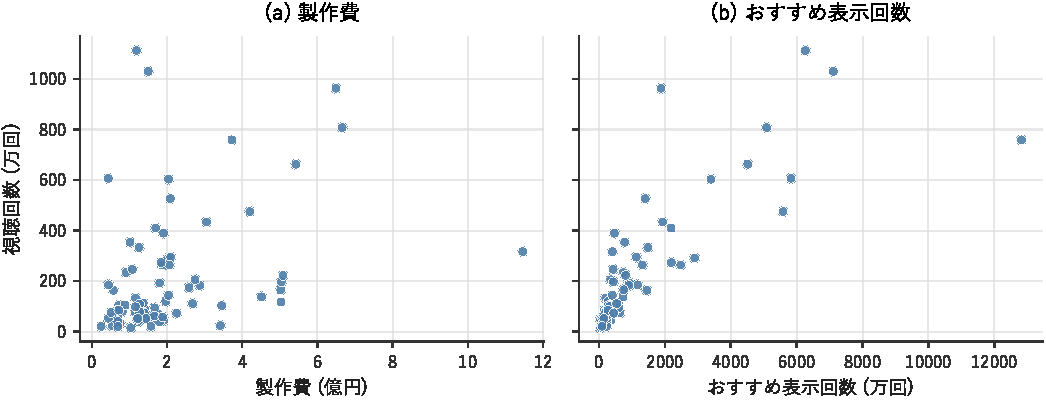
\includegraphics[width=\linewidth]{../figures/output/ch08_actual_scatter.pdf}
  \caption{80本の製作費／おすすめ表示回数と視聴回数の散布図. 1点が1作品を表す. 縦軸の尺度は共通だが, 横軸の単位と尺度は左右で異なる.}
  \label{fig:ch08-actual-scatter}
\end{figure}

では, 視聴回数とより強く連動しているのは, 製作費とおすすめ表示回数のどちらだろう.
2枚を並べて見比べても, どちらとも言えない.
横軸の単位も範囲も違う2枚の図では, 点の散らばり方をそのまま比べられないからだ.
おまけに, 散布図の印象は描き方ひとつで変わる.
同じデータでも, 縦軸を引き伸ばせば点の散らばりが縦に広がって関係が強そうに見えるし, 横軸を引き伸ばせば同じ理屈で弱そうに見える.
目で言えるのは, せいぜい「どちらも右上がり」までだ.

「一緒に動いている度合い」を, 目ではなく数で測れないだろうか.


\subsection{偏差の積から相関係数へ}

\subsubsection*{「一緒に動く」を偏差で捉える}

2つの変数$X$と$Y$が「一緒に動いている」とは, どういう状態のことだろうか.

もし$X$と$Y$が無関係なら, $X$が平均より大きい作品を選んでも, その作品の$Y$は大きいことも小さいこともあって, 規則性はない.
一方, $X$が平均より大きいときに$Y$も平均より大きい傾向があるなら, 二つは同じ方向に動いているといえる.
「一緒に動く」の中身は, 平均より上か下かという方向の一致らしい.

方向の一致なら, 第2章の偏差で捉えられそうだ.
ある値が平均より大きければ偏差は正, 小さければ負.
偏差の符号が, 平均より上か下かをそのまま表している.
そこで, $X$の偏差$(X - E[X])$と$Y$の偏差$(Y - E[Y])$を掛け合わせてみる.
両方が正なら, 積は正になる.
両方が負でも, 負$\times$負で積は正だ.
符号が食い違うときだけ, 積は負になる.
つまり偏差の積は, 一つのデータ点について「二つの変数が平均に対して同じ側にいるか, 逆の側にいるか」を符号で答える.

すべてのデータ点についてこの積を計算し, 平均をとってみる.
同じ側にいる点が多ければ平均は正に, 逆の側にいる点が多ければ負に傾く.
データ全体として同じ方向に動く傾向が強いのか, 逆方向の傾向が強いのかが, 1つの数値に集約される.

\subsubsection*{共分散の定義}

この考え方を式にしたものが\textbf{共分散}である.

\begin{defi}[]{共分散}{covariance}
2つの変数$X$, $Y$に対し, 共分散$\mathrm{cov}(X,Y)$を
\[
\mathrm{cov}(X,Y) = E[(X - E[X])(Y - E[Y])]
\]
と定義する.
\end{defi}

$(X - E[X])$は$X$の平均からのずれ, $(Y - E[Y])$は$Y$の平均からのずれで, その積の平均$E[\cdot]$をとっている.
第2章で学んだ分散の定義
\[
V(X) = E[(X - E[X])^2]
\]
と並べてみると, 分散は同じ変数の偏差どうしを掛けて平均したもの, 共分散は異なる変数の偏差どうしを掛けて平均したものだ.
分散の考え方を2変数に広げた量といえる.

共分散が正なら, $X$が大きいときに$Y$も大きい傾向がある.
負なら, $X$が大きいときに$Y$は小さい傾向がある.
0に近ければ, 同じ側と逆の側が打ち消し合っていて, どちらの傾向も強くない.

\subsubsection*{共分散の値は単位しだいで変わる}

符号が方向を表すなら, 値の大きさは連動の強さを表していそうだ.
確かめるために, 同じデータの単位だけを変えて, 共分散を計算し直してみる.
製作費を円で測るか, 万円で測るか.
円から万円への換算は1万で割るだけだが, 製作費の偏差も1万分の1になるから, 偏差の積も, その平均である共分散も1万分の1になる.
測っている作品は同じ, 視聴回数もそのままなのに, 製作費の単位を変えただけで, 共分散の値は1万分の1に変わってしまう.

値そのものがこれだけ動くと, 大きさの比較には使えない.
「製作費と視聴回数の共分散は1200, おすすめ表示回数と視聴回数の共分散は85」と並べられても, 製作費のほうが強く連動しているとは言えない.
1200と85の違いは, 連動の強さの違いではなく, 単位の違いを反映しているだけかもしれないからだ.

単位の影響を消して, 連動の強さだけを取り出したい.

\subsubsection*{ピアソンの相関係数}

第2章で学んだ標準偏差は, データが平均のまわりにどれくらい散らばるかを, データと同じ単位で表す量だった.
共分散を, $X$の標準偏差$\sigma_X$と$Y$の標準偏差$\sigma_Y$で割ってみる.
製作費を円から万円に変えると共分散は1万分の1になるが, 製作費の標準偏差も1万分の1になる.
分子と分母が同じだけ縮むので, 割った結果は変わらない.
単位の影響が, ここで消える.

こうして得られる量が\textbf{ピアソンの相関係数}$\rho$だ.

\begin{defi}[]{ピアソンの相関係数}{pearson-correlation}
2つの変数$X$, $Y$の標準偏差を$\sigma_X = \sqrt{V(X)}$, $\sigma_Y = \sqrt{V(Y)}$とする. ただし$\sigma_X > 0$かつ$\sigma_Y > 0$とする. ピアソンの相関係数$\rho_{XY}$を
\[
\rho_{XY} = \frac{\mathrm{cov}(X,Y)}{\sigma_X \, \sigma_Y}
\]
と定義する. $\rho_{XY}$は$-1$以上$1$以下の値をとる.
\end{defi}

分子は偏差の積の平均, 分母はそれぞれのばらつきの大きさの積だ.
単位の影響が分子と分母で打ち消し合うので, 製作費と視聴回数のペアでも, おすすめ表示回数と視聴回数のペアでも, 同じ尺度の上で値を読める.

別の見方もできる.
各変数をあらかじめ標準化して, 平均0, 標準偏差1に揃えてから共分散をとる, と考えてもよい.
標準化した変数を
\[
Z_X = \frac{X - E[X]}{\sigma_X}, \quad Z_Y = \frac{Y - E[Y]}{\sigma_Y}
\]
とすれば,
\[
\rho_{XY} = E[Z_X Z_Y]
\]
と書ける.
$Z_X$は「$X$が平均から標準偏差何個分離れているか」を表す, 単位のない量だ.
製作費が円でも万円でも, 標準偏差何個分かに直してしまえば同じ値になる.
相関係数は, 標準化した変数どうしの共分散だと言い直せる.

\subsubsection*{なぜ\texorpdfstring{$-1$}{-1}と\texorpdfstring{$1$}{1}の間に収まるのか}

定義には, $\rho_{XY}$が$-1$以上$1$以下の値をとると書いた.
積の平均なのだから, 平均から大きく離れた値どうしの積が重なれば, いくらでも大きくなりそうな気もする.
それでも$1$を超えられないのは, なぜだろうか.

手がかりは, $Z_X$と$Z_Y$の「食い違い」を測ってみることにある.
2つの量がどれだけ食い違っているかを見たいなら, 差を二乗して平均すればよい.
ずれを二乗して平均するという, 分散と同じ発想だ.
\[
E[(Z_X - Z_Y)^2] = E[Z_X^2] - 2E[Z_X Z_Y] + E[Z_Y^2]
\]
右辺は, $(a-b)^2 = a^2 - 2ab + b^2$という見慣れた展開の各項に, 期待値をとったものだ.
そして, 右辺の部品はすべて正体がわかっている.
$Z_X$は平均0だから, $E[Z_X^2]$は$Z_X$の分散そのものであり, 標準化で1に揃えてある.
$E[Z_Y^2]$も同じく1だ.
真ん中の$E[Z_X Z_Y]$は, さきほど見たとおり$\rho_{XY}$そのものだった.
代入すると,
\[
E[(Z_X - Z_Y)^2] = 1 - 2\rho_{XY} + 1 = 2(1 - \rho_{XY})
\]
となる.
左辺は二乗した量の平均だから, どんなデータでも0より小さくはならない.
すると右辺の$2(1 - \rho_{XY})$も0以上でなければならず, $\rho_{XY}$は1を超えられない.

では, ちょうど1になるのはどんなときか.
左辺が0になるとき, つまり$Z_X$と$Z_Y$の食い違いがまったくないときだ.
「相関係数が1」とは, 標準化した2つの変数が完全に重なっている状態のことだったのだ.

$-1$の側も同じ理屈で出る.
$Z_Y$の符号を反転した$-Z_Y$との食い違いを測れば, $E[(Z_X + Z_Y)^2] = 2(1 + \rho_{XY})$が0以上であることから, $\rho_{XY}$は$-1$を下回れない.
等号が成り立つのは$Z_X$と$-Z_Y$が完全に重なるとき, つまり2つの変数が完全に逆向きに連動しているときだ.
その間の値は, 完全な重なりと完全な逆向きのあいだの, 部分的な重なりの度合いを表している.

$-1$から$1$という範囲は, このように式から必然的に出てくる.
一方で, 標準偏差で割って尺度を揃えるという設計そのものは, 単位の違うペアどうしを比較したいという人間の都合で選ばれたものであって, 自然に決まる唯一の定義ではない.

\subsubsection*{\texorpdfstring{$\rho$}{ρ}の値と散布図の対応}

$\rho = 1$のとき, すべてのデータ点が完全に1本の右上がり直線の上に乗る.
$X$が増えれば$Y$も必ず増え, 例外は1点もない.
$\rho = -1$なら, 完全な右下がりの直線だ.

$|\rho|$が1から離れるにつれて, 点は直線から散らばり始める.
$\rho = 0.8$なら, 右上がりの傾向は明確だが, 直線からはみ出す点がちらほらある.
$\rho = 0.3$あたりになると, 右上がりの傾向はあるにはあるが, 散らばりが大きく, ぱっと見では判別しにくい.
$\rho = 0$では, 点の配置に方向性がなく, 雲のように広がる.
\cref{fig:ch08-correlation-examples}では, 軸の尺度を揃えてこの違いを並べた.

\begin{figure}[htbp]
  \centering
  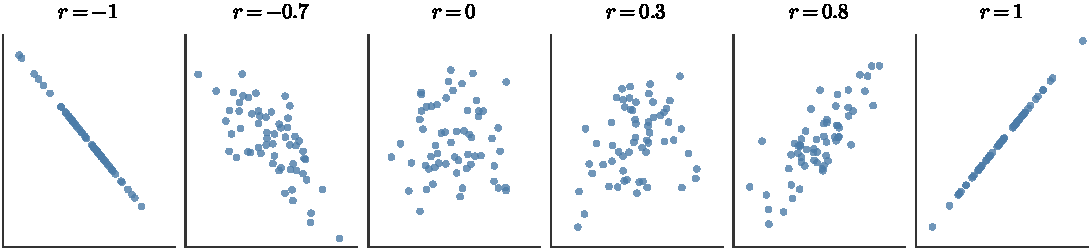
\includegraphics[width=\linewidth]{../figures/output/ch08_correlation_examples.pdf}
  \caption{相関係数 $r=-1,-0.7,0,0.3,0.8,1$ に対応する散布図. 各図は平均0, 標準偏差1に揃えた60点の合成データである.}
  \label{fig:ch08-correlation-examples}
\end{figure}

$|\rho|$が測っているのは, 点の並びが1本の直線にどれだけ近いか, である.

ただし, 直線への近さと直線の\textbf{傾き}は別の量だ.
ゆるやかな右上がりでも, 急な右上がりでも, 点が直線の上に乗っていれば$\rho = 1$になる.
相関係数が表すのは点がどれだけ直線に集まっているかであって, その直線がどれだけ急かではない.


\subsection{標本データからの計算手順}

ここまでの$\rho$は, 期待値$E[\cdot]$で書かれた母集団の性質だ.
実際に手元にあるのは, $n$個のデータの組$(x_1, y_1), (x_2, y_2), \ldots, (x_n, y_n)$である.
この標本から相関係数を計算する手順を追っていく.

なお, この計算には前提が2つある.
各データ点$(x_i, y_i)$が互いに独立に得られていることと, 調べたいのが2変数の直線的な関係であることだ.
前提から外れたデータで何が起きるかは, 本章の後半で確かめる.

\subsubsection*{手順}

計算は6つのステップで進む.
どのステップも, 前節の理論のどこかの部品に対応している.

\subsubsection*{ステップ1：平均を求める.}
\[
\bar{x} = \frac{1}{n} \sum_{i=1}^{n} x_i, \qquad \bar{y} = \frac{1}{n} \sum_{i=1}^{n} y_i
\]
これが「中心」の基準になる.

\subsubsection*{ステップ2：各データの偏差を求める.}
各$i$について$(x_i - \bar{x})$と$(y_i - \bar{y})$を計算する.
平均からどちらの方向にどれだけ離れているかが, ここで数値になる.

\subsubsection*{ステップ3：偏差の積を計算する.}
各$i$について$(x_i - \bar{x})(y_i - \bar{y})$を求める.
同方向のずれなら正, 逆方向なら負だ.
共分散の「中身」にあたる部分である.

\subsubsection*{ステップ4：偏差の積を合計し, 標本共分散を求める.}
\[
u_{xy} = \frac{1}{n-1} \sum_{i=1}^{n} (x_i - \bar{x})(y_i - \bar{y})
\]
分母は$n$ではなく$n-1$になっている.
第2章の脚注で触れた不偏分散と同じ理由で, 標本から母集団の共分散を偏りなく推定するために$n-1$で割る.

\subsubsection*{ステップ5：各変数の標本標準偏差を求める.}
\[
u_x = \sqrt{\frac{1}{n-1} \sum_{i=1}^{n} (x_i - \bar{x})^2}, \qquad u_y = \sqrt{\frac{1}{n-1} \sum_{i=1}^{n} (y_i - \bar{y})^2}
\]

\subsubsection*{ステップ6：標本相関係数を計算する.}
\[
r = \frac{u_{xy}}{u_x \, u_y}
\]
母集団の$\rho$に対応する標本からの推定値として, $r$を用いる.
分子と分母には同じ $n-1$ が含まれ, 比を取ると約分される.
したがって, $n-1$ で割る定義に揃えても相関係数の値は変わらない.

計算表を作って手で追うと, 偏差の符号がそのまま積の符号に現れる.
あわせて, 平均から大きく離れたデータの組は積の絶対値が大きく, 合計を強く引っ張る.
この性質は, 本章の後半でもう一度出てくる.

手順が揃ったところで, 実際のデータに当てはめる.


\subsection{三つの相関を比べる}

冒頭の問いに戻る.
視聴回数とより強く連動しているのは, 製作費とおすすめ表示回数のどちらか.
配信サービスの邦画作品の標本で, 実際に計算してみる.
3つの結果を先に\cref{fig:ch08-actual-correlations}へ並べる.

\begin{figure}[htbp]
  \centering
  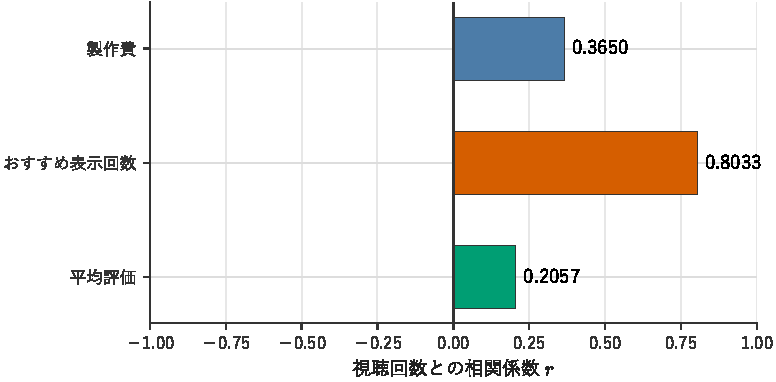
\includegraphics[width=0.8\linewidth]{../figures/output/ch08_actual_correlations.pdf}
  \caption{80本の実データから計算した, 視聴回数とのピアソンの標本相関係数. 3変数は単位が異なるが, 相関係数なら同じ尺度で比較できる.}
  \label{fig:ch08-actual-correlations}
\end{figure}

製作費と視聴回数の相関係数は, 前節の手順で計算すると $r = 0.3650$ となる.
弱から中程度の正の相関である.
散布図で見えていた右上がりの印象に, 数字がついた.
製作費の大きい作品ほど視聴回数も多い傾向はあるが, 点が1本の直線に沿って並ぶほどの強さではない.

同じ手順で, おすすめ表示回数と視聴回数の相関係数を計算すると, $r = 0.8033$ となる.
こちらは強い正の相関である.
冒頭では答えられなかった比較が, ここでは言い切れる.
単位も範囲もまるで違う2つのペアが, 同じ$-1$から$1$の物差しに乗っているからだ.
視聴回数との連動は, 製作費よりおすすめ表示回数のほうがはっきり強い.

もう一つ, 平均評価（5段階評価の平均値）と視聴回数の相関も計算してみると, $r = 0.2057$ で, こちらは弱い.
評価の高い作品ほど多く見られている, という素朴な期待は, 部分的にしか当たっていない.

3つの相関を並べると, 同じ「視聴回数との関係」でも, 相手の変数によって強さがかなり違う.
視聴回数は, 作品の中身や評判だけでなく, 配信側がどれだけ表示するかという配置に強く結びついているらしい.


\subsection{強い相関は因果を意味しない}

おすすめ表示回数と視聴回数の強い相関を見ると, おすすめ表示を増やせば視聴回数が伸びる, と読みたくなる.
だが, 相関係数が示しているのは, 二つの変数が連動しているという事実までだ.
連動していることと, 一方が他方の原因であることは, 別の話である.

有名な例がある.
夏になると, アイスクリームの売上が増える. 同じ時期に, 水難事故の件数も増える.
月ごとに集計すれば, アイスの売上と水難事故の件数には強い正の相関が出るはずだ.
だからといって, アイスを食べると溺れやすくなるわけではない.
両方を同時に動かしているのは\textbf{気温}という第三の変数だ.
気温が上がればアイスは売れるし, 海やプールに行く人が増えて事故も増える.

このように, 背後の共通の原因が二つの変数を同時に動かしているために生まれる相関を\textbf{擬似相関}と呼ぶ.
共通の原因にあたる変数は\textbf{交絡因子}という.
アイスと水難事故なら誰も因果を疑わないが, もっともらしい組み合わせで同じ構造が現れると, 気づくのは難しい.

おすすめ表示回数と視聴回数の場合は, 擬似相関とはまた別の難しさもある.
「おすすめに表示されたから視聴された」のか, 「よく視聴された作品が, 人気があると判断されてさらに表示された」のか.
どちらの向きでも, 観測される相関は同じ正の値になる.
相関係数は連動の強さを測るだけで, どちらが先でどちらが後か, という向きの情報を含んでいない.

相関からわかるのは, 「関係がありそうだ」という手がかりまでだ.
因果を主張するには, 第三の変数の影響を断つ設計（たとえば実験や条件の統制）や, 時間の前後関係の確認が別に必要になる.
この点は第10章で改めて扱う.


\subsection{相関係数だけではわからないこと}

相関係数は, 二つの変数の散らばり方を1つの数値に要約している.
第2章で見たとおり, 要約すれば落ちる情報がある.
そして, 落ちた情報が結論を左右することもある.

\subsubsection*{\texorpdfstring{$\rho = 0$}{ρ = 0}でも関係がないとは限らない}

$Y = X^2$という関係を考えてみる.
$X$が$-3$から$3$まで対称に散らばっているとすると, $X$が負のときも正のときも, 絶対値が大きければ$Y$は大きい.
散布図を描けば, きれいなU字型が現れる.
$X$を決めれば$Y$が決まるのだから, 関係としてはこの上なく強い.
ところが, 相関係数を計算すると, ほぼ0になる.
$X$が負の側では偏差の積が負に, 正の側では正になり, 対称に散らばっているせいで打ち消し合うからだ.

前に見たとおり, 相関係数が測っているのは, 点の並びが直線にどれだけ近いかだった.
U字のような曲がった関係は, どれだけ強くても$\rho$の値には現れない.
$\rho$が0に近いことから言えるのは「直線的な関係が見当たらない」までで, 「関係がない」ではない.

\subsubsection*{たった1点で値が変わる}

次の10個のデータ点で相関係数を計算すると, $r \approx 0.05$になる.
\[
(1,6),\; (2,1),\; (3,7),\; (4,5),\; (5,8),\; (6,3),\; (7,10),\; (8,9),\; (9,2),\; (10,4)
\]
\cref{fig:ch08-outlier}の左側を見ても, 点はほぼランダムに散らばっていて, 直線的な関係は見当たらない.

ここに, 他の点からかけ離れた$(22, 22)$という1点を追加して, 11個で計算し直すと, $r \approx 0.76$になる.
ほぼ無相関だった10点が, 1点増えただけで, かなり強い正の相関に読める数値に変わった.

\begin{figure}[htbp]
  \centering
  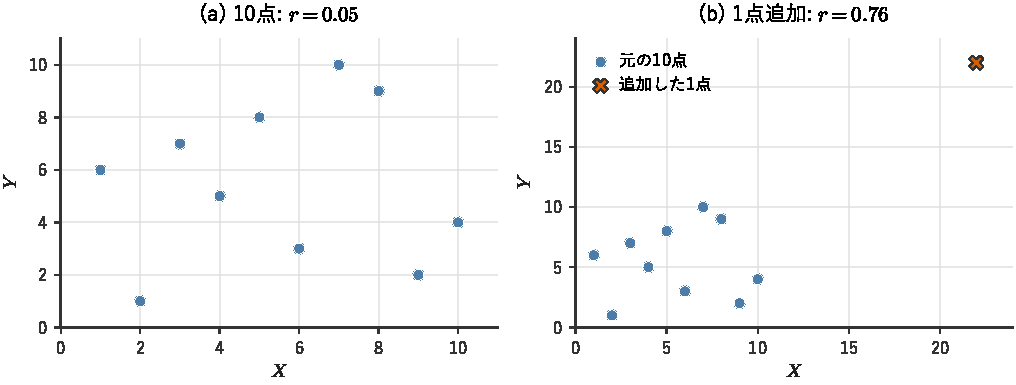
\includegraphics[width=0.9\linewidth]{../figures/output/ch08_outlier.pdf}
  \caption{外れ値を加える前後の散布図. 左は10点で $r=0.05$. 右は同じ10点に $(22,22)$ を加えた11点で $r=0.76$. 元の10点を読み取れるよう, 左右で軸の範囲を変えている.}
  \label{fig:ch08-outlier}
\end{figure}

原因は, 計算手順の節で見た偏差の積の性質にある.
$(22, 22)$はどちらの変数でも平均から大きく離れているから, この1点の偏差の積が, 他の10点の積の合計よりはるかに大きい.
$r \approx 0.76$という値は, 事実上この1点が決めている.

数値だけを見ていたら, そのことには気づけない.
散布図には, 10点の無秩序な散らばりと, ぽつんと離れた1点が, そのまま見えている.

\subsubsection*{部分と全体で向きが逆になる}

ある大学の2つの学部で, 勉強時間と試験の成績の関係を調べたとする.
学部Aの学生30人で計算すると$r = 0.7$, 学部Bの学生30人でも$r = 0.6$.
どちらの学部でも, 勉強時間が長い学生ほど成績がよい.
ところが, 2学部の60人をまとめて計算し直すと, $r \approx -0.3$という負の値になることがある.

\begin{figure}[htbp]
  \centering
  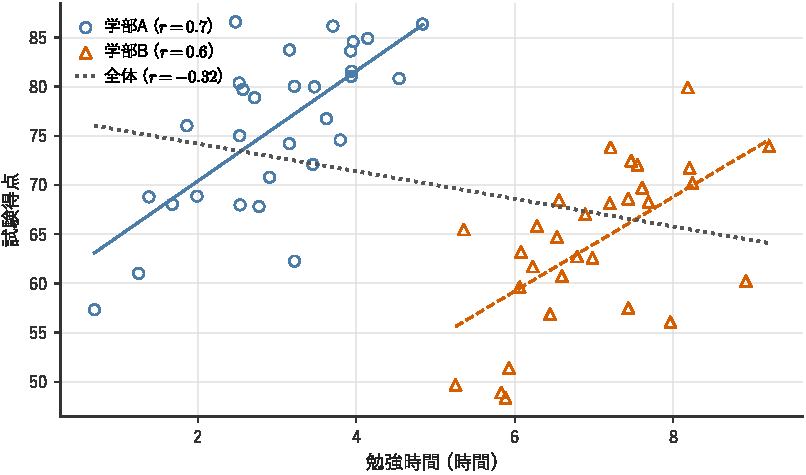
\includegraphics[width=0.8\linewidth]{../figures/output/ch08_simpson.pdf}
  \caption{シンプソンのパラドックスを示す合成データ. 学部Aと学部Bは各30人で, 群内の相関はそれぞれ $r=0.700$, $r=0.600$. 2群をまとめると $r=-0.316$ になる. 点の形と線種でも群と回帰直線を区別した.}
  \label{fig:ch08-simpson}
\end{figure}

原因は, 2つの群の平均の位置にある.
学部Aが平均的に勉強時間が短く成績の高い集団で, 学部Bが平均的に勉強時間が長く成績の低い集団だったとする.
60人まとめて計算すると, 偏差の基準になる平均は2つの群の中間に来る.
すると学部Aの学生の多くは「勉強時間が平均より短く, 成績は平均より高い」側に, 学部Bの学生の多くはその逆側に入り, 偏差の積は負に傾く.
各学部の中の右上がりの傾向より, 群と群の位置関係のほうが強く効いてしまうのだ.

この現象は\textbf{シンプソンのパラドックス}と呼ばれる.
集計の仕方しだいで, 相関の向きまで変わりうるという例である.
そしてここでも, \cref{fig:ch08-simpson}を見れば, 右上がりの2つのかたまりが離れた場所に並んでいる様子がそのまま見えている.

\vspace{1em}

U字も, 離れた1点も, 2つのかたまりも, 相関係数の数値だけでは見分けがつかない.
散布図には, どれもそのまま見えている.
散布図だけでは連動の強さを比べられなかったように, 相関係数だけでは散らばりの姿がわからない.
散布図で姿を確かめ, 相関係数で強さを測る. どちらか一方では足りない.

\begin{mybox}{カール・ピアソンと相関係数の歴史}
相関係数を体系的に定式化したのは, イギリスの統計学者カール・ピアソン（1857--1936）である.\footnotemark
ピアソンは, フランシス・ゴルトンが親子の身長データから見出した「回帰」の考え方を数学的に整備し, 相関係数の計算法を確立した.

しかし, ピアソンは優生学の熱心な推進者でもあった.
彼が相関係数を発展させた動機の一つは, 遺伝的特徴の親子間の「関係の強さ」を測ることにあり, その成果は優生政策の正当化にも使われた.
相関係数という数式そのものは中立でも, どんな問いに対して, どんな意図で使うかによって, 結果の意味はまったく変わる.

統計の手法を学ぶときは, 「それで何ができるか」だけでなく, 「それがどう使われてきたか」にも目を向ける価値がある.
\end{mybox}
\footnotetext{%
相関係数の定式化は Pearson, K. (1896). Mathematical Contributions to the Theory of Evolution. III. Regression, Heredity, and Panmixia. \textit{Philosophical Transactions of the Royal Society of London. Series A}, 187, 253--318.}


\subsection{測れたものと, まだ測れていないもの}

本章では, 二つの量が一緒に動く度合いを, 偏差の積から組み立てた.
偏差の積の平均が共分散になり, それぞれの標準偏差で割ると, 単位によらない$-1$から$1$の尺度になる.
単位の違う3つの変数について視聴回数との相関を並べ, おすすめ表示回数がいちばん強く, 製作費は弱いながらも正, 平均評価はさらに弱い, という順序まで確かめられた.

ここで言えたのは, 連動の向きと強さまでだ.
おすすめ表示が視聴回数を押し上げているのか, 視聴された作品がさらに表示されやすくなるのか, その向きは相関係数からは決められなかった.
そして, 製作費と視聴回数に弱い正の相関があるとわかっても, 製作費を増やしたら視聴回数がどれだけ変わるのか, という量については, まだ何も言えていない.



\newpage


\section{回帰 : 関係を直線で表し, 予測に使う}

\subsection{問い : 製作費を増やしたら, 視聴回数はどのくらい変わるか}

前章では, 製作費と視聴回数のあいだに, 弱いながらも正の相関があることを相関係数で確かめた.
製作費の大きい作品ほど, 視聴回数も多い傾向にある.

この相関係数を手がかりに, もう一歩踏み込めないだろうか.
たとえば, ある作品の製作費を1千万円積み増したとき, 視聴回数がどれだけ伸びるのかを見積もりたい.
ところが, 相関係数をどう眺めても, その数字は出てこない.
相関係数は$-1$から$1$のあいだの, 単位のない数だ.
二つがどれくらい一緒に動くかは表しても, 片方を1つ動かしたときにもう片方がいくつ動くか, という量までは含んでいない.

そこで, 前章で描いた散布図に戻ってみる.
製作費と視聴回数の点が, 右上がりにばらついている.
この点の並びを, 1本の直線でなぞってみる.
すると, その傾きが, 製作費が1つ増えるごとに視聴回数が平均していくつ増えるかにあたる.
相関係数に足りなかったのは, この傾きの情報だったわけだ.

では, その1本の直線は, どうやって引けばいいのだろう.


\subsection{素朴な方法と限界 : 目で引いた線は当てになるか}

散布図に直線を1本引くだけなら, 定規があれば足りそうだ.
ところが, 実際に定規を当ててみると, 意外なところで手が止まる.
点は少しずつずれた場所に散らばっていて, すべての点の上を通る直線は引けない.
どんな線を引いても, どこかの点は線から外れる.
右上の点に寄せれば左下の点から離れるし, 全体の真ん中を狙えば, どの点にも微妙に合わない.
どの外れを我慢して, どの点に寄せるか.
それを決めるものがないまま, なんとなくの1本を引くことになる.

このなんとなくは, 人によって違う.
同じ散布図でも, 右端に離れた点を重視する人は急な線を引き, 中央の密集に合わせる人はゆるやかな線を引く.

つまり, 目分量の線には2つの問題がある.
「良い直線」とは何かの\textbf{基準がない}こと.
そして, 基準がないせいで誰が引くかによって線が変わり, \textbf{再現性がない}ことだ.

そこで, 「良い直線」とは何かの基準を, 先に決めることにする.
基準が決まれば, どの1本が最も良いかは目分量ではなく計算で決まり, 誰がやっても同じ線になる.


\subsection{外れの大きさで直線を選ぶ : 残差と最小二乗法}

\subsubsection*{直線の式 : \texorpdfstring{$y = a + bx$}{y = a + bx}}

2変数$x$と$y$の間に直線的な関係があると想定して,
\[
  y = a + bx
\]
という形でその関係を表すことを考える.

$b$は\textbf{傾き}だ.
$x$が1増えたとき, $y$が平均的にいくつ変わるかを表す.
製作費と視聴回数の例なら, $b$ は「製作費が1単位増えたときに視聴回数が平均何単位増えるか」を表す.

$a$は\textbf{切片}で, $x = 0$のときの$y$の値にあたる.
ただし, $x = 0$が現実的な意味を持たない場合も多い.
製作費がゼロの作品が実際にはありえないのなら, 切片の数値そのものにこだわる必要はない.
直線の位置を決めるために数学的に必要な部品だと思えばよい.

問題は, この$a$と$b$をどう決めるかだ.

\subsubsection*{残差 : 外れを数にする}

前の節で決め手を欠いたのは, 点の「外れ」を目分量のまま扱っていたからだ.
そこでまず, 外れを数にする.
$i$番目のデータ点$(x_i, y_i)$に対して, 直線が予測する値は$a + bx_i$だ.
実際の値$y_i$とこの予測値の差を\textbf{残差}と呼び, $e_i$と書く.

\begin{defi}{残差}{residual}
データ点$(x_i, y_i)$と回帰直線$y = a + bx$に対し,
\[
  e_i = y_i - (a + bx_i)
\]
を$i$番目の\textbf{残差}と呼ぶ.
\end{defi}

$e_i$が正なら, 実際の値が直線より上にある.
負なら, 直線より下にある.
残差は, 直線がその点をどれだけ外したかの記録だ.
すべての点を通る直線が引けない以上, 残差をゼロにはできない.
ならば, 残差がなるべく小さい直線を「良い直線」と呼ぶことにすればよさそうだ.

では, $n$個ある残差が「全体として小さい」とはどういう状態だろうか.
残差をそのまま合計すると, 正と負が打ち消し合ってゼロに近づいてしまう.
第2章で分散を定義したときも, 偏差の合計がゼロになるのを防ぐために二乗した.
ここでも同じ手を使う.
各残差を\textbf{二乗}してから合計する.

\subsubsection*{最小二乗法 : 残差の二乗和を最小にする}

この「残差の二乗和を最小にする$a$と$b$を選ぶ」という方針に名前がついている.

\begin{defi}{最小二乗法}{ols}
$n$個のデータ$(x_1, y_1), \ldots, (x_n, y_n)$に対し,
\[
  S(a, b) = \sum_{i=1}^{n} e_i^2 = \sum_{i=1}^{n} (y_i - a - bx_i)^2
\]
を最小にする$a$と$b$を選ぶ方法を\textbf{最小二乗法}（OLS: Ordinary Least Squares）と呼ぶ.
\end{defi}

$S(a, b)$は残差の二乗和だ.
$a$と$b$の値が変われば$S$の値も変わる.
探すのは, $S$を最小にする$a$と$b$の組だ.

とはいえ, 動かせる文字が2つある.
高校で二次関数の最小値を求めたときは, 動く文字は1つだった.
2つ同時に相手にするのは難しそうなので, 片方を止めて1つずつ調べることにしよう.

\subsubsection*{切片が先に決まる}

まず, 傾き$b$を適当な値に固定して, 切片$a$だけを動かす.
$S$の中身を$a$に注目して並べ直すと,
\[
  S = \sum_{i=1}^{n} \bigl( (y_i - bx_i) - a \bigr)^2
\]
と読める.
$b$は止めてあるから, $y_i - bx_i$の部分は$n$個の決まった数だ.
つまり$S$は, 決まった数それぞれから$a$を引いて, 二乗して足したものになっている.
展開して$a$について整理すると,
\[
  S = n a^2 - 2\left(\sum_{i=1}^{n}(y_i - bx_i)\right) a + \sum_{i=1}^{n}(y_i - bx_i)^2
\]
となり, $S$は$a$の二次関数だとわかる.
しかも$a^2$の係数は$n$で, 必ず正だ.
グラフは下に凸の放物線だから, 底がただ1か所あって, そこで$S$は最小になる.
底の位置は平方完成で求められる.
二次関数$pt^2 - 2qt + r$（$p > 0$）は, 平方完成すると$p\left(t - \frac{q}{p}\right)^2 + (\mbox{定数})$の形になるから, 底は$t = \frac{q}{p}$にある.
当てはめると,
\[
  a = \frac{1}{n}\sum_{i=1}^{n}(y_i - bx_i) = \frac{1}{n}\sum_{i=1}^{n}y_i - b \cdot \frac{1}{n}\sum_{i=1}^{n}x_i = \bar{y} - b\bar{x}
\]
のとき$S$は最小になる.
最も良い切片は, $n$個の数$y_i - bx_i$の平均だったわけだ.

この式は, 見た目以上のことを言っている.
$a = \bar{y} - b\bar{x}$を直線の式$y = a + bx$に戻すと, $x = \bar{x}$のとき$y = \bar{y}$になる.
つまり, 傾きをどう選ぼうと, 最良の切片を選んだ直線は必ず点$(\bar{x}, \bar{y})$, データの重心にあたる点を通る.
最良の直線の候補は, 重心を通る直線だけに絞られた.
残る問題は, 重心をどんな傾きで通り抜けるかだけだ.

\subsubsection*{傾きの公式を導く}

$a = \bar{y} - b\bar{x}$を$S$に代入して整理すると,
\[
  S = \sum_{i=1}^{n} \bigl( (y_i - \bar{y}) - b(x_i - \bar{x}) \bigr)^2
\]
となる.
残ったのは, $y$の偏差と$x$の偏差, そして傾き$b$だけの式だ.
各項の二乗を開いて, $b$の次数ごとにまとめる.
二乗を開いて部品を調べるこの手は, 前章で相関係数が$\pm 1$に収まる理由を確かめたときにも使った.
\[
  S = \left( \sum_{i=1}^{n}(x_i - \bar{x})^2 \right) b^2
      - 2\left( \sum_{i=1}^{n}(x_i - \bar{x})(y_i - \bar{y}) \right) b
      + \sum_{i=1}^{n}(y_i - \bar{y})^2
\]
ごつい見た目になったが, 3つの係数はどれもデータから計算できる決まった数で, 動くのは$b$だけだ.
$S$はまたしても二次関数になった.
$b^2$の係数は偏差の二乗の和だから正で, グラフは下に凸の放物線だ.
さきほどの$pt^2 - 2qt + r$と同じ形で, $p$にあたるのが$\sum(x_i - \bar{x})^2$, $q$にあたるのが$\sum(x_i - \bar{x})(y_i - \bar{y})$になっている.
底は$t = q/p$, つまり
\[
  b = \frac{\displaystyle\sum_{i=1}^{n}(x_i - \bar{x})(y_i - \bar{y})}{\displaystyle\sum_{i=1}^{n}(x_i - \bar{x})^2}
\]
のとき$S$は最小になる.

まとめると, 残差の二乗和を最小にする直線はただ1本で, その傾きと切片は
\[
  b = \frac{\displaystyle\sum_{i=1}^{n}(x_i - \bar{x})(y_i - \bar{y})}{\displaystyle\sum_{i=1}^{n}(x_i - \bar{x})^2}, \qquad a = \bar{y} - b\bar{x}
\]
と, データから直接計算できる.

傾き$b$の分数の部品は, 前章で出会ったものばかりだ.
分子の$\sum(x_i - \bar{x})(y_i - \bar{y})$は, $x$と$y$の偏差の積の合計だ.
前章の共分散の分子と同じ構造をしている.
分母の$\sum(x_i - \bar{x})^2$は$x$の偏差の二乗和で, $x$の分散の分子にあたる.

つまり傾き$b$は, 「$x$と$y$がどれだけ一緒に動くか」を「$x$自身の散らばり」で割ったものだ.
$x$が1単位散らばるごとに, $y$が平均的にどれだけ動くか.
公式はそう読める.

ここで, 前の節で挙げた2つの問題を思い出そう.
「良い直線」の基準がないことと, 誰が引くかで線が変わってしまうことだった.
「残差の二乗和を最小にする」という基準は, 人間が選んだ約束だ.
偏差の二乗で散らばりを測った第2章の分散と同じで, 自然にそう決まるわけではない.
残差を絶対値で測る方法も考えられるが, それだと$S$は二次関数にならず, いま使った平方完成の手が通らない.
二乗なら, 見てきたとおり答えが1つの式にまとまる.
そして, 基準さえ約束してしまえば, どの直線が最良かは二次関数の底として一意に決まり, そこに人間の裁量はもう入らない.
基準は人間が決め, その基準の下での答えは数学が決める.
だから, 誰が計算しても同じ1本の線が出る.

\begin{mybox}{ガウスとケレスの軌道}
1801年, イタリアの天文学者ピアッツィが小惑星ケレスを発見した.
しかし観測できたのはわずか41日間で, ケレスは太陽の向こう側に隠れてしまった.
再び姿を現したときにどこにいるかを, 不完全な観測データから予測しなければならない.
ガウスは観測値と予測値のずれの二乗和を最小にする方法で軌道を推定し, その予測は的中した.
ケレスは予測された位置で再発見された.

最小二乗法は, 「手元にあるのは不完全なデータだが, そこから最も確からしい答えを引き出したい」という切実な動機のもとで実用化された.
なお, フランスのルジャンドルが1805年に最小二乗法を先に公表しており, 優先権を巡る論争がある.
ガウスは「自分は1795年から使っていた」と主張したが, 出版が後だったため決着はついていない.
\end{mybox}


\subsubsection*{相関係数との関係}

傾き$b$の式と前章の相関係数$r$の式を見比べると, 次の関係が導かれる.
\[
  b = r \cdot \frac{s_y}{s_x}
\]

$r$は関係の強さと方向を$-1$から$1$で表す, 単位のない指標だった.
$s_y / s_x$は, $y$の散らばりが$x$の散らばりの何倍かを表している.
単位のない「連動の度合い」に散らばりの比を掛けると, 「$x$が1単位増えたとき$y$がいくつ変わるか」という単位つきの量に変わる.
前章の相関係数と本章の傾きは, 同じ直線関係を別の角度から見た量だったわけだ.


\subsection{引いた直線を疑う : \texorpdfstring{$R^2$}{R²}と残差プロット}

最小二乗法は, どんな点の散らばりに対しても, 残差の二乗和が最小になる1本を必ず選び出す.
点が直線とは呼べない並び方をしていても, 計算は止まらず, 傾きと切片の数字が出てくる.
選ばれた1本が候補の中で最も外れの小さい線であることは, さきほどの導出が保証している.
しかし, その「最も小さい外れ」が小さいとはかぎらない.
最もましな線と, 良い線は別物だ.
だから, 引いた直線がどのくらい信用できるかは, 引いたあとに確かめる必要がある.

\subsubsection*{\texorpdfstring{$R^2$}{R²} : 説明できた割合}

手がかりは, 最小化のあとに残ったものにある.
残差の二乗和$S$は, 最小にはなったが, ゼロになったわけではない.
残った$S$は, 直線がどうしても拾いきれなかった散らばりの量だ.
この残りが小さいのか大きいのかを測りたい.

ただ, $S$の値をそのまま見ても, 判断はつかない.
視聴回数を「回」で数えるか「万回」で数えるかで, 値は何桁も変わってしまうからだ.
共分散をそのままでは比べられず, 標準偏差で割って相関係数にしたのと同じ事情で, 比べる相手が要る.

そこで, 直線を引く前の外し方と比べることにする.
もし$x$の情報がまったくなかったとしたら, $y$の値をどう予測するだろうか.
使えるのは$\bar{y}$, つまり$y$の平均しかない.
どのデータ点に対しても$\bar{y}$と答えるしかないから, 予測は当然はずれる.
各点と$\bar{y}$のずれの二乗和$\sum(y_i - \bar{y})^2$が, $y$の全体の散らばりだ.
この量を$\mathrm{SS_{total}}$と呼ぶ.

回帰直線を引くと, 予測値が$\bar{y}$から$\hat{y}_i = a + bx_i$に変わる.
$x$の情報を使ったぶんだけ, 予測は改善されるはずだ.
それでも残るずれの二乗和$\sum(y_i - \hat{y}_i)^2$を$\mathrm{SS_{res}}$と呼ぶ.
中身は, 最小二乗法で最小にしたあの$S$の, 最小値そのものだ.
$\mathrm{SS_{total}}$は$x$を知らないときの誤差で, $\mathrm{SS_{res}}$は$x$を使ったあとの誤差だ.
この2つを比べて, $x$の情報で誤差がどれだけ減ったかを測る.

\begin{defi}{決定係数}{r-squared}
$y$の全変動を$\mathrm{SS_{total}} = \sum(y_i - \bar{y})^2$, 残差による変動を$\mathrm{SS_{res}} = \sum(y_i - \hat{y}_i)^2$とする.
決定係数は
\[
  R^2 = 1 - \frac{\mathrm{SS_{res}}}{\mathrm{SS_{total}}}
\]
で定義される. $\hat{y}_i = a + bx_i$は回帰直線による予測値である.
\end{defi}

$\mathrm{SS_{res}} / \mathrm{SS_{total}}$は, 直線で説明しきれなかった散らばりの割合だ.
1から引けば, 「説明できた割合」に変わる.

$R^2 = 0.76$なら, $y$の散らばりの76\%が$x$との直線関係で説明でき, 残り24\%は直線では捉えきれていない.
$R^2 = 1$なら全点が直線上に乗っており, $R^2 = 0$なら$x$と$y$に線形関係がない.

ここまで読んで, 「0.76は良いのか悪いのか」と思ったかもしれない.
正直に言えば, 分野による.
物理の実験データなら$R^2 = 0.76$は低すぎるかもしれないし, 人間の行動データや社会調査なら十分に高い.
「この値以上なら合格」という普遍的な基準はない.
$R^2$は他のモデルや他のデータとの比較に使う相対的な指標だと思っておくのがよい.

単回帰では, $R^2$は相関係数$r$の二乗に一致する.
$r = 0.87$なら$R^2 = 0.87^2 \approx 0.76$だ.
前章で「相関が強い」と評価したことと, 本章で「76\%説明できた」と評価することが, 数値としてつながっている.

\subsubsection*{\texorpdfstring{$R^2$}{R²}だけでは安心できない}

$R^2$が高ければ直線がデータをよく捉えている, と言いたくなる.
しかし, $R^2$は残差の大きさを1つの数値に圧縮した要約だ.
圧縮する過程で, ずれ方のパターンが消える.
数の要約だけでは分布の形が見えないことは第2章で確かめ, 失われた形は図で取り戻すのだと第3章でやった.
同じことが, 直線への当てはまりにも起きる.

アンスコムのカルテットという有名な例がある.
4組のデータ（各11点）のすべてで, $r \approx 0.82$, $R^2 \approx 0.67$, 傾きも切片もほぼ同じだ.
数値だけ見たら, 4組とも「まあまあの直線関係」で片づけてしまうだろう.

ところが散布図を描くと, 実態はまるで違う.

% [図挿入: アンスコムのカルテットの4枚の散布図]

1組目は素直な直線関係で, 回帰直線がデータをよく捉えている.
2組目は完全な放物線で, 直線を当てはめること自体が不適切だ.
3組目はほぼ完璧な直線に外れ値が1点だけあり, その1点が傾きを歪めている.
4組目は$x$が1点だけ離れた位置にあり, その1点が見かけの相関を作り出している.

1973年にフランシス・アンスコムがこの4組を発表した意図は明確だ.
統計量を計算する前にグラフを描け, ということだ.
$R^2$や傾きの数値だけでは, データの本当の姿はわからない.

\subsubsection*{残差プロット : 残差の形を目で見る}

では, 何の図を描けばよいか.
疑っている相手は「直線の外し方」だから, 見るべきは残差そのものだ.
残差$e_i = y_i - \hat{y}_i$を, 予測値$\hat{y}_i$に対してプロットした図を\textbf{残差プロット}と呼ぶ.

なぜ横軸が$x_i$ではなく$\hat{y}_i$なのかと思うかもしれない.
単回帰では$\hat{y}_i = a + bx_i$だから, 横軸を$x_i$にしても$\hat{y}_i$にしても図の形は変わらない.
ただ, 説明変数が複数ある重回帰では$x$が1つに決まらないため, $\hat{y}$を使うのが慣例だ.
本書では単回帰だけを扱うが, 慣例に合わせておく.

直線がデータの関係をうまく捉えていれば, 残差はゼロのまわりにランダムに散らばる.
逆に, 残差に系統的なパターンが見えたら, 直線では捉えきれない構造がデータに残っている.

残差プロットで確認するのは2点だ.

\begin{itemize}
  \item \textbf{パターンがあるか}. U字型が見えたら, 本当は曲線的な関係なのに直線で無理に近似した可能性がある. 扇形に広がっていれば, 予測値が大きい領域で予測が不安定になっている.
  \item \textbf{飛び離れた点があるか}. 他の残差から大きく外れた点があれば, そのデータ点を個別に確認する.
\end{itemize}

U字型が見えた場合にどうするか.
典型的な対処は, 二次関数などの曲線モデルを検討するか, データの範囲を絞って直線が妥当な区間だけを使うことだ.
本書では直線モデルの範囲にとどめるが, 直線でうまくいかないときにも出口はある.

残差の量は$R^2$で測り, 残差の形は残差プロットで見る.
この2つが, 引いた直線を疑うときの基本の確かめになる.


\subsection{実践 : 製作費と視聴回数で問いに答える}

章の冒頭で, 製作費を積み増したら視聴回数はどれだけ伸びるのか, という問いを立てた.
前章で扱った, 配信サービスの邦画作品の標本から製作費と視聴回数の組を10件取り出して, 直線を引き, その直線を疑い, 問いに数字で答えるところまで通してみよう.
以下の表の数値は, 計算手順を見せるための仮置きであって, ランニングデータの実値とは別物である（実値はランニングデータ確定後に置き換える）.

\subsubsection*{Step 1 : 散布図の確認}

まず, データの全体像を確認する.

\begin{center}
\begin{tabular}{crr}
\hline
$i$ & 製作費 $x_i$（仮単位） & 視聴回数 $y_i$（仮単位） \\
\hline
1 & 20 & 140 \\
2 & 25 & 200 \\
3 & 30 & 215 \\
4 & 40 & 180 \\
5 & 45 & 245 \\
6 & 50 & 200 \\
7 & 55 & 260 \\
8 & 65 & 255 \\
9 & 70 & 310 \\
10 & 80 & 295 \\
\hline
\end{tabular}
\end{center}

% [図挿入: 製作費 vs 視聴回数の散布図]

散布図を描くと, 右上がりの傾向が見える.
ただし, 点はきれいに並んでいるわけではない.
たとえば$i = 4$（製作費40, 視聴回数180）は周囲より低く, $i = 5$（製作費45, 視聴回数245）は高い.
同じような製作費でも視聴回数には幅がある. 相関が1ではないというのは, 散布図の上ではこの幅のことだ.
大きな曲がりや極端に飛び離れた点は見当たらないので, 直線を当てはめることに無理はなさそうだ.

\subsubsection*{Step 2 : 傾きと切片の計算}

公式に代入するために, まず平均を求める.
\[
  \bar{x} = \frac{20 + 25 + \cdots + 80}{10} = \frac{480}{10} = 48, \qquad
  \bar{y} = \frac{140 + 200 + \cdots + 295}{10} = \frac{2300}{10} = 230
\]

次に, 各データの偏差と, その積を計算する.
面倒に見えるが, 表にすれば機械的に進む.

\begin{center}
\begin{tabular}{crrrrr}
\hline
$i$ & $x_i$ & $y_i$ & $x_i - \bar{x}$ & $y_i - \bar{y}$ & $(x_i - \bar{x})(y_i - \bar{y})$ \\
\hline
1 & 20 & 140 & $-28$ & $-90$ & 2520 \\
2 & 25 & 200 & $-23$ & $-30$ & 690 \\
3 & 30 & 215 & $-18$ & $-15$ & 270 \\
4 & 40 & 180 & $-8$ & $-50$ & 400 \\
5 & 45 & 245 & $-3$ & 15 & $-45$ \\
6 & 50 & 200 & 2 & $-30$ & $-60$ \\
7 & 55 & 260 & 7 & 30 & 210 \\
8 & 65 & 255 & 17 & 25 & 425 \\
9 & 70 & 310 & 22 & 80 & 1760 \\
10 & 80 & 295 & 32 & 65 & 2080 \\
\hline
 & & & & 計 & 8250 \\
\hline
\end{tabular}
\end{center}

同様に$\sum(x_i - \bar{x})^2$を求めると, $784 + 529 + 324 + 64 + 9 + 4 + 49 + 289 + 484 + 1024 = 3560$となる.

これで部品が揃った. 公式に代入する.
\[
  b = \frac{8250}{3560} \approx 2.32, \qquad a = 230 - 2.32 \times 48 \approx 118.6
\]

回帰直線は$y \approx 119 + 2.3x$と表せる.

% [図挿入: 散布図に回帰直線を重ねたもの]

傾き$b \approx 2.3$は, 「製作費を1単位増やすと, 視聴回数が平均的に約2.3単位増える」と読める.
相関係数だけではわからなかった「いくつ変わるか」が, この1つの数字に入っている.
冒頭の問いへの答えは, ひとまずこの形で出た.

切片$a \approx 119$は, 式の上では「製作費がゼロのとき視聴回数は約119」となる.
しかし, データの製作費は20から80の範囲に収まっている.
製作費ゼロの作品は実データに存在しない.
この119は直線の位置を決めるために計算上現れた数値であって, 「製作費を一切かけなくても119の視聴回数が出る」と解釈するのは危うい.

\subsubsection*{Step 3 : \texorpdfstring{$R^2$}{R²}で当てはまりを確認する}

最小二乗法は, どんなデータからでも1本の線を出すのだった.
出てきた数字をどこまで信じてよいかを, まず$R^2$で確かめる.

仮にこの仮置きデータで$r = 0.87$と求めたとすれば, $R^2 = 0.87^2 \approx 0.76$だ.
視聴回数の散らばりの約76\%が, 製作費との直線関係で説明できている.
残りの24\%は製作費だけでは説明しきれない.
おすすめ表示回数, 評価件数, ジャンル, 公開時期など, 他の要因が混ざっているのだろう.
表の$i = 4$（製作費40なのに視聴回数180）や$i = 6$（製作費50で視聴回数200）のように, 直線から大きくずれた作品がそれにあたる.
なお, 実際のランニングデータでは製作費と視聴回数の相関はもっと弱め（おおむね $r$ で 0.3〜0.5 程度）になる想定で, $R^2$ もこれより小さい値になる.

\subsubsection*{Step 4 : 残差プロットを確認する}

各データ点の予測値$\hat{y}_i = 119 + 2.3 x_i$と残差$e_i = y_i - \hat{y}_i$を計算すると, 次のようになる.

\begin{center}
\begin{tabular}{crrrrr}
\hline
$i$ & $x_i$ & $y_i$ & $\hat{y}_i$ & $e_i$ \\
\hline
1 & 20 & 140 & 165 & $-25$ \\
2 & 25 & 200 & 177 & 23 \\
3 & 30 & 215 & 188 & 27 \\
4 & 40 & 180 & 211 & $-31$ \\
5 & 45 & 245 & 223 & 22 \\
6 & 50 & 200 & 234 & $-34$ \\
7 & 55 & 260 & 246 & 14 \\
8 & 65 & 255 & 269 & $-14$ \\
9 & 70 & 310 & 280 & 30 \\
10 & 80 & 295 & 303 & $-8$ \\
\hline
\end{tabular}
\end{center}

% [図挿入: 残差プロット]

残差の符号は$-, +, +, -, +, -, +, -, +, -$で, 正と負が入り混じっている.
U字型のパターンや, 右に行くほど広がる扇形も見えない.
ゼロのまわりにランダムに散らばっていると判断してよい.
この直線モデルは, おおむね妥当だ.

\subsubsection*{予測 : できることと, やってはいけないこと}

疑いをひととおり通過した直線は, まだ見ていない作品の視聴回数の見積もりに使える.
「製作費が50の作品の視聴回数はおよそ$119 + 2.3 \times 50 \approx 234$」と見積もれる.
50はデータの範囲（20から80）に収まっているから, この予測にはそれなりの根拠がある.

同じ式に製作費200を入れても, 計算は止まらず, $119 + 2.3 \times 200 = 579$という数字が出てくる.
しかし, 200はデータの範囲をはるかに超えた値だ.
直線関係がそこまで続いている保証はない.
現実を考えても, 製作費には効果の頭打ちがある.
予算を2倍にしたからといって視聴回数が2倍になるとは限らない.

データの範囲外に直線を延ばして予測すること, いわゆる外挿は, 「直線が無限に続く」という仮定を暗に置いている.
その仮定が正しい保証はどこにもない.

前章の因果の議論も, ここでそのまま当てはまる.
$b \approx 2.3$は「製作費が1単位多い作品は視聴回数も平均約2.3単位多い」という関係を記述しているだけであり, 「製作費を増やせば視聴回数が増える」という因果を証明しているわけではない.
回帰にできるのは関係の記述と, その記述に基づく予測までで, 因果の証明は守備範囲の外にある.


\subsection{直線を引いた先に残る問い}

本章では, 相関係数の先にあった問い, 「$x$が変わったとき$y$はどのくらい変わるか」に答えた.

最小二乗法で直線を引き, 傾き$b \approx 2.3$から「製作費が1単位多い作品は視聴回数も平均約2.3単位多い」という量的な関係を読み取った.
$R^2 \approx 0.76$でその直線の説明力を確認し, 残差プロットで直線を信用してよいかを目で判断した.
前章では「関係がある」までだった答えが, 「1単位あたり約2.3」という数字まで進んだ.

振り返ると, 章の半分は線の引き方ではなく, 引いた線の疑い方に使った.
最小二乗法はどんなデータからでも1本の線を出すから, 出てきた数字を信じてよいかは, 残差の量と形を確かめてはじめて言える.
線を引いて終わりにせず, 残差を読むところまでが回帰の手続きだ.

ただし, 最小二乗法にも$R^2$にも前提がある.
$x$と$y$の関係がおおむね直線的であること.
各データ点が互いに独立であること.
極端な外れ値がないこと.
前提が崩れていれば, 直線を引いて数字は出るが, その数字は当てにならない.

たとえば, もしデータ点が独立でないのに独立だと仮定して回帰すると, 残差にパターンが現れ, $R^2$が実際の説明力より高く出るかもしれない.
回帰直線の数字を眺めても, そのことには気づけない.
これは直線を引く技術の問題ではなく, データの設計と解釈の問題だ.

前提が崩れる場面は意外と多い.
標本の集め方に偏りがあれば, 回帰直線も偏る.
因果の方向を取り違えていれば, 回帰の解釈そのものが間違う.
次章では, 第2章から本章まで積み上げてきた手法の前提を整理し, その前提が崩れるとどうなるかを体系的に確認する.
あわせて, バイアスの類型と, データを扱うときの倫理も扱う.
手法の「外側」を知ることが, 手法を正しく使うための最後の一歩になる.



\newpage
%\input{data_driven_decision_making.tex}

\section{統計の限界とバイアス : 手法の外側を知る}

\subsection{正しく計算しても結論が間違うとき}

前章の終わりに, 手法の外側を知ることが手法を正しく使うための最後の一歩になる, と書いた.
その外側で何が起こるのかは, 1つの実例を見るのが早い.

1973年, カリフォルニア大学バークレー校の大学院は, 性別を理由に女子受験生を差別しているとして訴えられた.
証拠とされたのは合格率の差だ. 全志願者を集計すると, 男子の合格率は約44\%, 女子は約35\%. 差は9ポイントある.
この数字を見て, 大学院に問題があると判断した人は当時多かった.

ところが大学院側が学部別に集計し直してみると, 数字の様子が変わる.
6つの主要学部のうち4つで, 女子の合格率は男子と同じか, むしろ高かった.
残り2つも, 全体集計に出ていた9ポイント差ほど大きな男子有利ではない.
学部単位で見るかぎり, 「女子の方が合格しにくい」と言える証拠はどこにも見当たらない.
それなのに, 大学全体の合計だけが男子有利に出る.

なぜそんなことが起こるのか.
学部ごとの合格率が, そもそも大きく違っていた.
人文系の合格率は20\%から30\%, 理工系は60\%から70\%という具合に, 学部間で2倍3倍の差がある.
そして女子は前者の「狭き門」に多く志望し, 男子は後者の「広き門」に多く志望していた.
各学部の中では公平でも, 女子が狭き門の学部に集中していたために, 全体平均では女子の合格率が下に引かれる.

集計の単位を変えただけで結論が逆転する. このような現象を\textbf{シンプソンのパラドックス}と呼ぶ.
平均は2章で, 割合は5章で扱った. どの計算も正しい.
それでも, 全体集計と学部別の集計で正反対のことが言える.

ただし, 集計の単位そのものが結論を狂わせたのではない.
学部によって合格率が大きく違い, 学部選びに男女差があった. この2つが重なって, 「学部」という第三の変数が性別と合格率の両方に絡んでいた.
全体集計はその第三の変数を隠し, 学部別の集計は表に出す. 結論を分けたのは, 集計の単位の裏で隠れたり現れたりしていた第三の変数のほうだ.
群によって混ざり方の違う第三の変数がある場面なら, 同じ逆転は平均の比較でも割合の比較でも起こりうる.

2章から9章までの手法は, 手順どおりに計算すれば誰がやっても同じ数字を返す. それでも結論が間違うのなら, 歪みは計算の外から入っている.
1章で述べたとおり, 標本には母集団のすべての情報が入らない. 特定の対象への偏りが生じるかどうかは, データの集め方による. だからこそ, 計算結果だけでなく, どのように集めたデータなのかも点検しなければならない. 本章では, 集め方から解釈までに入り込む歪みを, データの流れに沿って上流から順にたどる.
標本をどう集めたか. 集まったデータの中で何が観測できていたか. 出てきた数字をどう解釈したか.
シンプソンのパラドックスは, このうち最後の解釈の段階で起きた歪みにあたる. 集計の単位という解釈上の選択が, 結論を逆転させていた.
歪みの3類型を整理した後, 手法そのものが暗黙に置いている前提, そして数字の読み方の誤りへと進み, 最後に本書全体を振り返って閉じる.


\subsection{バイアスの3類型 : 上流・中流・下流の歪み}

3類型のうち最も身近なのは上流, 標本の集め方に入る歪みだ.

\subsubsection*{上流 : サンプリングバイアス}

5章の終わりに, \textbf{精密に間違える}という言葉が出てきた.
標本の集め方が偏っていると, $n$を増やすほど信頼区間は狭くなるのに, 区間の中心は的外れのままになる, という警告だった.
あの警告に, ここで名前をつける.

たとえば, 関心のある母集団は「日本に住む有権者」なのに, 集まったのが「平日の昼に渋谷駅にいた人」だったとしよう.
件数を10万人に増やしたところで, 平日の昼に渋谷駅にいない人の意見は最後までゼロのままだ.
標本平均が近づいていく先は, 知りたい「日本に住む有権者」の平均ではなく, 「平日の昼に渋谷駅にいた人たち」の平均でしかない.

これが\textbf{サンプリングバイアス}である.
標本が母集団を代表していないとき, 信頼区間は$n$を増やすほど狭く, しかも誤った位置に決まっていく.
件数を増やして解決できる問題ではない.

5章で紹介したリテラリー・ダイジェスト誌の大はずれも, 構図は渋谷駅と同じだった.
240万人という件数はギャラップの5万人を数十倍上回っていたのに, 電話帳と自動車登録簿から作った名簿が, 大恐慌下で電話も車も持たない貧困層をまるごと外していた.
ギャラップが勝ったのは件数ではなく, 標本の代表性で勝っていたからだ.

サンプリングバイアスの厄介さは, データの中身をいくら眺めても見抜けないところにある.
点検の対象は, 中身ではなく抽出の手順そのものだ.
確認するのは2点. 誰がリストに載っていたかという抽出枠と, 声を拾えた人と拾えなかった人を分ける回答率である.
ダイジェスト誌の調査なら, 「電話帳と自動車登録簿から抽出した」という1行に, 1936年の貧困層が入っていない事実がそのまま書かれている.
分析を始める前に, 抽出枠と回答率をまず確かめる. サンプリングバイアスの大半は, この入口の確認で見つかる.

\subsubsection*{中流 : 生存者バイアス}

抽出の枠組みの点検では捕まらない歪みもある.
「そもそも観測できなかったもの」の抜け落ちだ.

第二次大戦中, 米軍は帰還した爆撃機の被弾箇所を調べて, どこを補強すべきかを検討していた.
集計してみると, 翼の先端と機体後部に弾痕が集中していた.
最初の判断はこうだ. 「弾痕の多い場所を補強しよう」.

統計学者アブラハム・ワルドはこの結論に待ったをかけた.
補強すべきは弾痕の少ない場所のほうだ, と.
帰還した機は, 翼や機体後部に被弾しても飛び続けられた機だ.
エンジンや操縦席を被弾した機は, そもそも基地に戻ってこない.
分析の対象に上がっていたのは「生き残った機」だけで, 「生き残れなかった理由」がデータから抜けていた.

これが\textbf{生存者バイアス}である.
「観測できたものだけ」を見て結論を出すと, 観測できなかったものが体系的に抜け落ちる.
事業継続中の企業だけを集めて成功要因を語る研究, 在籍中の社員だけを集めた満足度調査, 完走したマラソン選手だけを集めた走法分析.
どれも, 退場した側に重要な情報が眠っている可能性がある.

点検の手順は, 手元のデータを見るより先に, 「ここに本当はどんな対象が含まれるべきか」を書き出すことだ.
書き出した母集団と実際に手元にあるデータの差が, 生存者バイアスの入る隙間にあたる.
その差を説明できないなら, 結論はその差の分だけ歪んでいる.

\subsubsection*{下流 : 確証バイアス}

3つめの歪みは, データではなく, 数字を読む人間の側に入る.
人間には, 自分の仮説に合うデータを重く受け取り, 合わないデータを軽く流す癖がある.
この癖を\textbf{確証バイアス}と呼ぶ.
心の持ちようの問題に聞こえるかもしれないが, 確証バイアスは統計の手続きの中にも入り込む.
選び方しだいで, 1つ1つの計算は正しいまま, 全体として嘘をつけてしまうからだ.
6章の検定を使って, その仕組みを具体的に見る.

公平なコインを20枚用意して, それぞれ100回ずつ投げ, 各コインで「表と裏の出方が偏っているか」を有意水準5\%で検定する場面を考えよう.
有意水準5\%とは, 6章で導入したとおり「本当は公平なのに偶然偏って見える確率を5\%まで許容する」という設定だ.
コイン1枚あたり, 偽陽性（公平なのに有意と判定される）が出る確率は5\%, 出ない確率は95\%である.
20枚を独立に検定するから, どの1枚も偽陽性を出さない確率は$0.95^{20}$. その裏返しで, どこかで偽陽性が出る確率は

$$
1 - (1 - 0.05)^{20} \approx 0.64
$$

つまり約64\%だ. 20回試せば, 6割以上の確率で「有意な発見」が偶然で生まれる.

ここで実験者が「有意になった1枚」だけを論文にし, 残り19枚を引き出しにしまったらどうなるか.
表に出るのは「特殊なコインを発見した」という主張だけだ.
6章で習ったp値の計算は, どの1枚についても正しく行われている.
1枚ごとの検定だけ見れば嘘はない.
それなのに, 「20枚試して当たりだけ報告した」という1段上の選別のせいで, 全体としての結論は嘘になる.

これが\textbf{p-ハッキング}と呼ばれる行為だ.
自分の仮説に合う結果だけを拾うという確証バイアスの癖が, ここでは検定という正式な手続きの上で動いている.
都合のいい結果が出るまで分析の角度や対象を変え続けると, 拾う作業に自覚すら要らなくなる.

抑える手順は2つ用意されている.
1つは事前登録. 何を, どんな仮説で, どの分析手順で見るかを, データを見る前に書いて第三者に渡しておく.
やってから決めるのではなく, やる前に決めてあるので, 「都合のいい結果が出てから条件を変える」という余地がふさがる.
もう1つは多重比較の補正. 同じデータで20回検定するなら, 各検定の有意水準を5\%でなく0.25\%程度に厳しくする（ボンフェローニ補正）か, 別の方法で「全体の偽陽性率」を抑える.
補正の詳細は本書の範囲を超えるが, 枠組みが用意されているので, 必要になった場面で調べ直せば足りる.

3類型は別々の知識ではなく, 標本の入手から解釈までの1本の流れの上の3地点である.
点検の時期も流れに沿う. 分析を始める前に抽出枠と回答率を確かめ, 手元のデータを前にしたら観測できなかったものを書き出し, 結果を読むときに選別の有無を疑う.


\subsection{手法の前提が崩れるとき : 独立性・線形性・等分散性}

データの集め方に歪みがなくても, 手法そのものは暗黙の前提に乗っている.
前章の終わりに, 最小二乗法と$R^2$の前提を3つ挙げた. 関係がおおむね直線的であること, データ点が互いに独立であること, 極端な外れ値がないこと.
このうち外れ値の怖さは, 1点が傾きを歪めるアンスコムの3組目として前章で既に見た.
ここでは残る2つ, 独立性と線形性に, 幅つきの話で効いてくる等分散性を加えた3つを, 回帰に限らず2章から9章の推論全体に関わる前提として点検する.
崩れていたときに何ができるかも, それぞれに添える.

\subsubsection*{独立性 : 隣の点と関係していないか}

4章のCLTの前提として「独立同分布」を導入した.
ここでの「独立」は, データ点どうしが互いに無関係であることを指す.
ある月のデータが翌月のデータに影響しているなら, それは独立ではない.

前章では製作費（説明変数）と視聴回数（目的変数）の作品データに対して回帰直線を引いた.
回帰の計算式は, 各データ点を独立に扱い, 残差の二乗和を最小化している.
ところが, データ点が独立でなかったらどうなるか.
たとえば同じシリーズの続編作品が複数本含まれていれば, それらの視聴回数は互いに似た値になりやすく, 隣どうしの残差は同じ符号をとりやすい.
時系列データの場合も同じで, ある月の値が翌月の値に影響していれば隣の残差が連動する.

残差が独立に動くとき, それぞれが上下にランダムに散らばるから, 残差全体の散らばりが「データの本当の不確かさ」をきちんと写し取る.
ところが残差が隣どうしで似ていると, 「実は独立に取り直せばもっと違う値が出るはずなのに, 連動して動いているせいで似た値しか観測されていない」状態になる.
散らばりの計算は観測されたものをそのまま反映するから, 連動を割り引いてはくれない.
結果として, 計算上のSEは本当の不確かさより小さくなる.

SEが小さいと信頼区間も狭く出るし, 6章のp値も小さく出る.
本当は不確かな結論が, 数字の上では確実そうに見えてしまう.

時系列データだけが該当するわけではない.
クラスごとの生徒, 同じ会社の社員, 同じ地域の住民. 集団内の点は互いに似ている傾向がある.
集団効果を無視して全員を独立だと扱うと, 同じ問題が起こる.

独立性が崩れていそうなときの対処は, 「独立でない構造を計算式の側に取り込む」ことだ.
時系列データには時系列モデル（AR・MAなど）が, 集団内で似ているデータには階層モデル（マルチレベル分析）が用意されている.
本書の範囲は「独立ではなさそうだ」と気づくところまでで, その先は手法の名前を頼りに調べがつく.

\subsubsection*{線形性 : 直線で表せる関係なのか}

直線モデルは「関係がおおむね直線で表せる」という前提の下で意味を持つ.
本当の関係が放物線, 指数, 周期的なものだったら, 直線を引いて得られるのは「もっとも近い直線」だけだ.
傾きや切片の数値は出るが, それらは現実の関係を要約していない.

前章で残差プロットを導入したとき, アンスコムの2組目の話をした.
4組のデータはどれも$r \approx 0.82$, $R^2 \approx 0.67$という似た数字を返したが, 2組目の実体はきれいな放物線で, 直線を当てはめること自体が不適切だった.

線形性が崩れているかどうかは, 残差プロットに目を向ければ見える.
予測値の小さい所と大きい所の両方で残差が正に偏り, 中央で負に偏っていれば, 関係はU字型だ.
逆向きのパターンも同じ警告にあたる.

線形性の確認は数値だけでは届かない.
$R^2$が0.7を超えていても, 残差プロットが系統的なパターンを示していれば直線モデルは合っていない.
逆に$R^2$が0.4でも, 残差にパターンがなければ, それはそれで意味のある直線関係だ.
$R^2$は当てはまりの「総量」しか語らず, 「外し方の質」は残差プロットでしかわからない.

崩れていたときの対処は, 関係の形に合わせて式を変えることだ.
$x^2$の項を加えて2次式にする. $\log x$を取って線形に直す. 周期成分があれば三角関数を加える.
線形回帰の計算自体は, 説明変数を増やしても同じ手順で実行できるから, 「直線でないなら捨てる」のではなく「形を変えて当てはめる」と思っておくと使いやすい.

\subsubsection*{等分散性 : 場所によって散らばりが違わないか}

3つめの前提が, 残差の散らばりがデータの位置によって変わらないこと, つまり等分散性である.
7章のt検定でWelch法を採ったのは, 2群間で分散が違うことを許す扱いを選んだという意味で, 等分散性の仮定を緩めた選択だった.

回帰では事情が少し違う.
たとえば, 予測値が大きい領域ほど残差の散らばりが広がるデータでは, 残差プロットに左側が狭く右側が広い扇形が現れる.
この扇形は, 等分散性が崩れたときの典型的な形の一つである.
第9章の残差プロットでも, 残差の幅が場所によって一定とは言いにくかった.
ただし, 大きな残差は予測値の小さい側にも現れており, 右へ広がる典型的な扇形ではなかった.
等分散性の崩れを疑う形は, 扇形だけではない.

このとき, 直線そのものは間違っていない.
平均的な傾きは正しく推定されている.
ただし, 「製作費を5億円に決めたら視聴回数はおよそいくつか」と幅つきで予測したい場合, 場所ごとに本当の散らばりが違うのに一律のSEで予測区間を出すと, 散らばりが小さい場所では広すぎ, 大きい場所では狭すぎる.
平均の推定は使えても, 予測の幅の保証は当てにならない. 「全部ダメ」ではなく「部分的にダメ」だ.

対処も独立性と線形性の場合と同じように用意されている.
残差の散らばりに合わせてSEを計算し直す方法（ロバスト標準誤差）と, 残差の大きい点を軽く扱う方法（重み付き最小二乗法）で, どちらも名前から調べがつく.

3つの前提の点検は, ほとんど残差プロット1枚に集約される.
残差を予測値に対してプロットし, ランダムに散らばっていればよし, 系統的なパターンや場所による幅の違いが見えたら警告.
前章で導入したあのプロットは, 線形回帰を使ってよいかどうかの確認手順を兼ねていたわけだ.


\subsection{数字の読み方を誤る典型 : p値・相関・外挿}

集め方にも手法の前提にも問題がないのに, 結論だけが間違う場面が残っている.
出てきた数字の読み方を誤る場合だ.
誤読が集中する場所は3か所に絞れる. p値, 相関と因果の関係, データ範囲の外側である.

\subsubsection*{p値の3つの誤読}

6章でp値を「帰無仮説が正しいと仮定したとき, 観測値以上に極端な結果が出る確率」と定義した.
この定義はそれなりに込み入っているせいで, 短く要約しようとすると意味がずれる.
ずれ方には型がある.

最初の誤読は, 「p値は帰無仮説が正しい確率である」という読み方だ.
これは違う. p値は「帰無仮説が正しいと仮定したとき」の珍しさを測っているのであって, 帰無仮説そのものの真偽の確率を返してくれるわけではない.
p値が0.03だからといって, 帰無仮説が正しい確率が3\%という意味にはならない.

次の誤読は, 「p<0.05なら効果は大きい」という読み方だ.
p値は珍しさの指標であって, 効果の大きさは別の指標で測る.
両者が別物である理由は, 「件数が増えると有意になりやすい」という性質に表れている.
4章で見たとおりSEは$u/\sqrt{n}$で, $n$が大きくなると小さくなる.
6章のt検定では検定統計量$t = \text{(2群の平均差)}/\text{SE}$だから, SEが小さくなれば$t$は大きくなる.
$t$が大きくなれば, 同じ平均差でもp値は小さく出る.
だから2群の平均差が小さくても, $n$が大きければ「珍しい」と判定される.
逆に$n$が小さければ, それなりに大きな差でも有意にならないことがある.

最後の誤読は, 「p>0.05なら効果はない」という読み方だ.
これも違う. 「珍しいと言える証拠が足りない」と「効果がないことが証明された」は別の話だ.
件数が少ない実験で有意にならなかったからといって, 効果が存在しないわけではない.

p値を扱うときは, p値だけで報告を済ませない方がよい.
5章の信頼区間と, 7章で触れた効果量を一緒に出す.
信頼区間は「効果がだいたいどの範囲にありそうか」, 効果量は「差そのものの大きさ」, p値は「偶然で説明しにくいかどうかの目安」.
3つはそれぞれ別の問いに答えている.

具体的な書き方の目安はこうだ.

\begin{quote}
2群の平均差は1.2点（95\%信頼区間 0.4から2.0）, 効果量（Cohenの$d$）は0.3, $p = 0.01$.
\end{quote}

平均差1.2点の周りに信頼区間が0.4から2.0と置かれているおかげで「効果は小さめだが正の方向は確かそうだ」と読み取れ, $d = 0.3$で「効果としては小さい部類」と相対化できる. p値はその仕上げに過ぎない.
報告するときはこの3点を並べる. 報告を読むときは, 3点が揃っているかをまず確かめる.

\subsubsection*{相関は因果ではない, ではどう違うのか}

相関が因果を意味しないことは, 8章で\textbf{擬似相関}と\textbf{交絡因子}という名前とともに確かめた.
アイスクリームの売上と水難事故の相関を作っていたのは, 両方を同時に動かす気温という第三の変数だった.
8章の終わりには, この点は第10章で改めて扱う, と書いた. その約束をここで果たす.

本章の冒頭のバークレーの話は, 交絡の実例そのものだ.
性別と合格率のあいだに「学部」という第三の変数が絡み, 直接の差別がない学部別の数字から, 全体では9ポイントの差が生まれていた.
気温のような物理量にかぎらず, 学部の選ばれ方, 国の面積や人口のような構造的な量まで, 両方の変数に絡むものは何でも交絡因子になりうる.
ヨーロッパ各国でコウノトリの巣の数と人間の出生数に正の相関が出るという有名な話も, 国の規模が両方を押し上げているだけである.

交絡を疑うときの確認手順は, 「両方を同時に押し上げそうな第三の変数」を1つ思いつくことから始まる.
思いついたら, その変数の値ごとにデータを分けて計算し直す. この手続きを\textbf{層別分析}と呼ぶ.
バークレーの大学院側がやったのは, まさにこの手続きだった. 学部で層別して合格率を出し直したら, 全体集計の男女差はほぼ消えた.
気温で層別したアイスと水難事故の相関も, 同じように消えるはずだ.
層別して消えれば交絡. 消えなければ, 別の説明を探すことになる.

その「別の説明」の筆頭が\textbf{逆因果}である.
$x$が$y$を動かしているのではなく, $y$が$x$を動かしている場合だ.
8章のおすすめ表示と視聴回数にも, この疑いがあった. 表示されたから視聴されたのか, よく視聴されたから表示が増えたのか.
「医療支出が多い地域ほど健康指標が悪い」というデータでも同じことが起こる.
医療支出が健康を損ねているのではなく, 健康状態が悪い地域だから医療支出が増えている, という向きの因果かもしれない.
矢印の向きを取り違えると, 結論はそのまま逆転する.

逆因果を疑うときの目印は時間順序だ.
$x$の変化は$y$の変化より先に起きているか.
データが同じ時点のスナップショットなら, 因果の向きは原理的に決まらない.
別の時点で同じ現象を測れたときに初めて, 矢印の向きを絞り込む手がかりが得られる.

交絡も逆因果もないのに強い相関が出ることもある. \textbf{偶然の一致}である.
無関係な2つの量を大量に集めて相関を計算すれば, そのうちのいくつかは偶然強く相関する.
「米国のチーズ消費量とベッドシーツでの絞死者数」のような, ふざけた相関の実例集が世間に出回っているくらいだ.
たくさん試せば偽陽性は出る. 本章の前半で見たp-ハッキングと同じ構造が, 相関の探索でも起こる.

偶然か本物かを切り分ける最低限の手は, 別のデータで再現するかを確かめることだ.
別の標本でも同じ強さの相関が出るなら本物の見込みが高い. 1度きりなら, 偶然の可能性は消えない.

交絡・逆因果・偶然は, 1つずつでも併発でも起こる.
相関を見たら問うことは3つ. 両方を押し上げる第三の変数はないか. 因果の向きは逆ではないか. 似たような量を大量に試した中の1つではないか.
1つでも即答できないうちは, 「強い相関がある」というだけで結論を下せない.

\subsubsection*{データの外側に踏み込むとき}

3つめの誤読は, 前章の終わりで一度通った場所にある.
製作費を億円, 視聴回数を万回で表した回帰直線$y \approx 108.4 + 49.4x$に製作費30億円を入れると, 視聴回数は約1590万回と計算される.
しかしデータの範囲は0.25億円から11.46億円で, そこで観測された直線関係が30億円まで続いている保証はどこにもない.
一定の額を超えると, 制作やプロモーションの仕組み自体が変わる場合もある.
範囲の外に直線を延ばす外挿は, 「直線が続いている」という根拠のない仮定を黙って置く行為なのだった.
切片$a \approx 108.4$を「製作費ゼロでも視聴回数108万回」と読めないのも同じ理由で, 製作費ゼロの付近にデータはなく, 108.4は直線の位置決めの計算から出た数値に過ぎない.

前章では回帰の話として出てきたが, 誤読の型として見ると, 外挿は回帰の直線に限らない.
過去3年の売上の伸び率を来年にそのまま延ばす. 20代への調査結果を全年代に広げて語る.
どちらも, 観測した範囲で成り立っていた関係を, 観測のない場所へ黙って持ち出している.

確認の手順は2つ.
語ろうとしている点が観測範囲の中にあるかを確かめる. 範囲の外を語るなら, 外挿であることを明記する.
数字が出ることと, その数字を現実に当てはめてよいことは別である.
モデルが関係を要約しているのは, 観測が届いた範囲までだ.


\subsection{本書の終わりに}

本書を1章から振り返ると, ずいぶん遠くまで来た.
要約から始めて, データの形を見て, ばらつきから幅を計算し, 群の差を吟味し, 関係を測り, モデルを当てはめ, そして本章で手法の外側にある歪みの見取り図を描いた.
学び始めの頃は, 計算結果を正しく出すことが目標だったかもしれない.
振り返ってみると, 正しく計算するのは出発点で, 本書の後半はずっと, 出てきた数字を疑う手順の話をしていた.
出した数字の前提は何か. 集計の単位は妥当か. 第三の変数を見落としていないか. 観測範囲の外まで延ばして語っていないか.
数字を出すたびにこの問いへ戻ってもらえるなら, 本書の役目はおおむね果たされている.

本書は統計の骨格に絞ったので, 各章で名前だけ挙げた話題には, それぞれ教科書1冊分の世界が広がっている.
多重比較の制御, ブートストラップ, 重回帰, 時系列モデルや階層モデルといった話題だ.
どの章で「もっと知りたい」と感じたか. その章の続きから手を伸ばすのが自然な順序だ.

最後にひとつ書いておきたい.
本書の手順を, 自分の手元のデータで, 最初から最後まで一度回してみてほしい.
その途中で引っかかった「ここはなぜそうなのか」が, 統計学の次の章への入口になる.

ここでいったん筆を置く. 続きは, 読者自身のデータの上で書かれる.


% \section{まとめとか：}


\end{document}

